%%%%%%%%%%%%%%%%%%%%%%%%%%%%%%%%%%%%%%%%%%%%%%%%%%%%%%%%%%%%%%%%%%%%%%%%%
%  Zawartość: Praca Dyplomowa Inżynierska - System do obsługi laboratorium
%  fotograficznego z możliwością sprzedaży foto usług online.
%  Opracował: Adam Dłubak <adam.dlubak@gmail.com>
%  Data: Listopad 2017
%  Wersja: 1.0
%%%%%%%%%%%%%%%%%%%%%%%%%%%%%%%%%%%%%%%%%%%%%%%%%%%%%%%%%%%%%%%%%%%%%%%%%

\documentclass[a4paper,onecolumn,oneside,12pt,extrafontsizes]{memoir}
% W celu przygotowania wydruku do archiwum należy przesłonić komendę powyższą
% dwoma poniższymi komendami:
%\documentclass[a4paper,onecolumn,twoside,10pt]{memoir} 
%\renewcommand{\normalsize}{\fontsize{8pt}{10pt}\selectfont}

%\usepackage[cp1250]{inputenc} % jeśli kodowanie edytowanych plików to cp1250 
\usepackage[utf8]{inputenc} % jeśli kodowanie edytowanych plików to UTF8
\usepackage[T1]{fontenc}
\usepackage[polish]{babel}
%\DisemulatePackage{setspace}
\usepackage{setspace}
\usepackage{tabularx}
\usepackage{color,calc}
\usepackage{xcolor,soul} % pakiet z komendami do podkreślania tekstu
\definecolor{xcolorsoulgrey}{rgb}{0.95,0.95,0.95}
\sethlcolor{xcolorsoulgrey}
\usepackage{wrapfig}
\usepackage{ebgaramond} % pakiet z czcionkami garamond, potrzebny tylko do strony tytułowej, musi wystąpić przed pakietem tgtermes

%% Aby uzyskać polskie literki w pdfie (a nie zlepki) korzystamy z pakietu czcionek tgterms. 
%% W pakiecie tym są zdefiniowane klony czcionek Times o kształtach: normalny, pogrubiony, italic, italic pogrubiony.
%% W pakiecie tym brakuje czcionki o kształcie: slanted (podobny do italic). 
%% Jeśli w dokumencie gdzieś zostanie zastosowana czcionka slanted (np. po użyciu komendy \textsl{}), to
%% latex dokona podstawienia na czcionkę standardową i zgłosi to w ostrzeżeniu (warningu).
%% Ponadto tgtermes to czcionka do tekstu. Wszelkie matematyczne wzory będą sformatowane domyślną czcionką do wzorów.
%% Jeśli wzory mają być sformatowane z wykorzystaniem innych czcionek, trzeba to jawnie zadeklarować.

%% Po zainstalowaniu pakietu tgtermes może będzie trzeba zauktualizować informacje 
%% o dostępnych fontach oraz mapy. Można to zrobić z konsoli (jako administrator)
%% initexmf --admin --update-fndb
%% initexmf --admin --mkmaps

\usepackage{tgtermes}   
\renewcommand*\ttdefault{txtt}

% We wcześniejszej wersji szablonu korzystano z innych czcionek. Dla celów historycznych pozostawiono je w komentarzu
%\usepackage{mathptmx} % pakiet będący następcą pakietów times and mathptm, niestety polskie literki są zlepkami
%\usepackage{newtxtext,newtxmath} % pakiety dostarczające Times dla tekstów i wzorów matematycznych,  
%                                  rozwiązuje problemy występujące w mathptmx, ale wymaga zainstalowania
%                                  dodatkowych pakietów oraz uruchomienia updmap (konsola administratora)
%                                  niestety polskie literki są zlepkami
%\usepackage{newtxmath,tgtermes} % można też połączyć czcionki do tekstu i czcionki do wzorów

\usepackage{listings} % pakiet do prezentacji kodu. 
%Wcześniej był problem z polskimi znakami w otoczeniu lstlisting, stąd pozostawiono w komentarzu zastosowane wtedy rozwiązanie: 
\lstset{literate=%-
{ą}{{\k{a}}}1 {ć}{{\'c}}1 {ę}{{\k{e}}}1 {ł}{{\l{}}}1 {ń}{{\'n}}1 {ó}{{\'o}}1 {ś}{{\'s}}1 {ż}{{\.z}}1 {ź}{{\'z}}1 {Ą}{{\k{A}}}1 {Ć}{{\'C}}1 {Ę}{{\k{E}}}1 {Ł}{{\L{}}}1 {Ń}{{\'N}}1 {Ó}{{\'O}}1 {Ś}{{\'S}}1 {Ż}{{\.Z}}1 {Ź}{{\'Z}}1 }%{\ \ }{{\ }}1}

\usepackage{color} %use color
\definecolor{mygreen}{rgb}{0,0.6,0}
\definecolor{mygray}{rgb}{0.5,0.5,0.5}
\definecolor{mymauve}{rgb}{0.58,0,0.82}
\definecolor{bluekeywords}{rgb}{0.13,0.13,1}
\definecolor{greencomments}{rgb}{0,0.5,0}
\definecolor{redstrings}{rgb}{0.9,0,0}

%Customize a bit the look
\lstset{ %
backgroundcolor=\color{white}, % choose the background color; you must add \usepackage{color} or \usepackage{xcolor}
basicstyle=\footnotesize, % the size of the fonts that are used for the code
breakatwhitespace=false, % sets if automatic breaks should only happen at whitespace
breaklines=true, % sets automatic line breaking
captionpos=b, % sets the caption-position to bottom
commentstyle=\color{mygreen}, % comment style
deletekeywords={...}, % if you want to delete keywords from the given language
escapeinside={\%*}{*)}, % if you want to add LaTeX within your code
extendedchars=true, % lets you use non-ASCII characters; for 8-bits encodings only, does not work with UTF-8
frame=single, % adds a frame around the code
keepspaces=true, % keeps spaces in text, useful for keeping indentation of code (possibly needs columns=flexible)
keywordstyle=\color{blue}, % keyword style
% language=Octave, % the language of the code
morekeywords={*,...}, % if you want to add more keywords to the set
numbers=left, % where to put the line-numbers; possible values are (none, left, right)
numbersep=5pt, % how far the line-numbers are from the code
numberstyle=\tiny\color{mygray}, % the style that is used for the line-numbers
rulecolor=\color{black}, % if not set, the frame-color may be changed on line-breaks within not-black text (e.g. comments (green here))
showspaces=false, % show spaces everywhere adding particular underscores; it overrides 'showstringspaces'
showstringspaces=false, % underline spaces within strings only
showtabs=false, % show tabs within strings adding particular underscores
stepnumber=1, % the step between two line-numbers. If it's 1, each line will be numbered
stringstyle=\color{mymauve}, % string literal style
tabsize=2, % sets default tabsize to 2 spaces
title=\lstname % show the filename of files included with \lstinputlisting; also try caption instead of title
}
%END of listing package%
 
\definecolor{darkgray}{rgb}{.4,.4,.4}
\definecolor{purple}{rgb}{0.65, 0.12, 0.82}
%define Javascript language
\lstdefinelanguage{JavaScript}{
keywords={typeof, new, true, false, catch, function, return, null, catch, switch, var, if, in, while, do, else, case, break},
keywordstyle=\color{blue}\bfseries,
ndkeywords={class, export, boolean, throw, implements, import, this},
ndkeywordstyle=\color{darkgray}\bfseries,
identifierstyle=\color{black},
sensitive=false,
comment=[l]{//},
morecomment=[s]{/*}{*/},
commentstyle=\color{purple}\ttfamily,
stringstyle=\color{red}\ttfamily,
morestring=[b]',
morestring=[b]"
}

\lstdefinelanguage{CSS}{
  morekeywords={accelerator,azimuth,background,background-attachment,
    background-color,background-image,background-position,
    background-position-x,background-position-y,background-repeat,
    behavior,border,border-bottom,border-bottom-color,
    border-bottom-style,border-bottom-width,border-collapse,
    border-color,border-left,border-left-color,border-left-style,
    border-left-width,border-right,border-right-color,
    border-right-style,border-right-width,border-spacing,
    border-style,border-top,border-top-color,border-top-style,
    border-top-width,border-width,bottom,caption-side,clear,
    clip,color,content,counter-increment,counter-reset,cue,
    cue-after,cue-before,cursor,direction,display,elevation,
    empty-cells,filter,float,font,font-family,font-size,
    font-size-adjust,font-stretch,font-style,font-variant,
    font-weight,height,ime-mode,include-source,
    layer-background-color,layer-background-image,layout-flow,
    layout-grid,layout-grid-char,layout-grid-char-spacing,
    layout-grid-line,layout-grid-mode,layout-grid-type,left,
    letter-spacing,line-break,line-height,list-style,
    list-style-image,list-style-position,list-style-type,margin,
    margin-bottom,margin-left,margin-right,margin-top,
    marker-offset,marks,max-height,max-width,min-height,
    min-width,-moz-binding,-moz-border-radius,
    -moz-border-radius-topleft,-moz-border-radius-topright,
    -moz-border-radius-bottomright,-moz-border-radius-bottomleft,
    -moz-border-top-colors,-moz-border-right-colors,
    -moz-border-bottom-colors,-moz-border-left-colors,-moz-opacity,
    -moz-outline,-moz-outline-color,-moz-outline-style,
    -moz-outline-width,-moz-user-focus,-moz-user-input,
    -moz-user-modify,-moz-user-select,orphans,outline,
    outline-color,outline-style,outline-width,overflow,
    overflow-X,overflow-Y,padding,padding-bottom,padding-left,
    padding-right,padding-top,page,page-break-after,
    page-break-before,page-break-inside,pause,pause-after,
    pause-before,pitch,pitch-range,play-during,position,quotes,
    -replace,richness,right,ruby-align,ruby-overhang,
    ruby-position,-set-link-source,size,speak,speak-header,
    speak-numeral,speak-punctuation,speech-rate,stress,
    scrollbar-arrow-color,scrollbar-base-color,
    scrollbar-dark-shadow-color,scrollbar-face-color,
    scrollbar-highlight-color,scrollbar-shadow-color,
    scrollbar-3d-light-color,scrollbar-track-color,table-layout,
    text-align,text-align-last,text-decoration,text-indent,
    text-justify,text-overflow,text-shadow,text-transform,
    text-autospace,text-kashida-space,text-underline-position,top,
    unicode-bidi,-use-link-source,vertical-align,visibility,
    voice-family,volume,white-space,widows,width,word-break,
    word-spacing,word-wrap,writing-mode,z-index,zoom, repeat, flex, -, align, items, justify},
  morestring=[s]{:}{;},
  sensitive,
  morecomment=[s]{/*}{*/}
}

\lstset{
language=[Sharp]C,
showspaces=false,
showtabs=false,
breaklines=true,
showstringspaces=false,
breakatwhitespace=true,
escapeinside={(*@}{@*)},
commentstyle=\color{greencomments},
keywordstyle=\color{bluekeywords},
stringstyle=\color{redstrings},
basicstyle=\ttfamily
}

 
\lstset{
language=JavaScript,
extendedchars=true,
basicstyle=\footnotesize\ttfamily,
showstringspaces=false,
showspaces=false,
numbers=left,
numberstyle=\footnotesize,
numbersep=9pt,
tabsize=2,
breaklines=true,
showtabs=false,
captionpos=b
}


% Choć możliwe jest zastosowanie różnych pakietów formatujących tabele, zaleca się tego nie robić.
%\usepackage{longtable}
%\usepackage{ltxtable}
%\usepackage{tabulary}

%%%%%%%%%%%%%%%%%%%%%%%%%%%%%%%%%%%%%%%%%%%%%%%%%%%
%% Ustawienia odpowiedzialne za sposób łamania dokumentu
%% i ułożenie elementów pływających
%%%%%%%%%%%%%%%%%%%%%%%%%%%%%%%%%%%%%%%%%%%%%%%%%%%
%\hyphenpenalty=10000		% nie dziel wyrazów zbyt często
\clubpenalty=10000      %kara za sierotki
\widowpenalty=10000  % nie pozostawiaj wdów
\brokenpenalty=10000		% nie dziel wyrazów między stronami
\exhyphenpenalty=999999		% nie dziel słów z myślnikiem
\righthyphenmin=3			% dziel minimum 3 litery

%\tolerance=4500
%\pretolerance=250
%\hfuzz=1.5pt
%\hbadness=1450

\renewcommand{\topfraction}{0.95}
\renewcommand{\bottomfraction}{0.95}
\renewcommand{\textfraction}{0.05}
\renewcommand{\floatpagefraction}{0.35}

%%%%%%%%%%%%%%%%%%%%%%%%%%%%%%%%%%%%%%%%%%%%%%%%%%%
%%  Ustawienia rozmiarów: tekstu, nagłówka i stopki, marginesów
%%  dla dokumentów klasy memoir 
%%%%%%%%%%%%%%%%%%%%%%%%%%%%%%%%%%%%%%%%%%%%%%%%%%%
\setlength{\headsep}{10pt} 
\setlength{\headheight}{13.6pt} % wartość baselineskip dla czcionki 11pt tj. \small wynosi 13.6pt
\setlength{\footskip}{\headsep+\headheight}
\setlength{\uppermargin}{\headheight+\headsep+1cm}
\setlength{\textheight}{\paperheight-\uppermargin-\footskip-1.5cm}
\setlength{\textwidth}{\paperwidth-5cm}
\setlength{\spinemargin}{2.5cm}
\setlength{\foremargin}{2.5cm}
\setlength{\marginparsep}{2mm}
\setlength{\marginparwidth}{2.3mm}
%\settrimmedsize{297mm}{210mm}{*}
%\settrims{0mm}{0mm}	
\checkandfixthelayout[fixed] % konieczne, aby się dobrze wszystko poustawiało
%%%%%%%%%%%%%%%%%%%%%%%%%%%%%%%%%%%%%%%%%%%%%%%%
%%  Ustawienia odległości linii, wcięć, odstępów
%%%%%%%%%%%%%%%%%%%%%%%%%%%%%%%%%%%%%%%%%%%%%%%%
\linespread{1}
%\linespread{1.241}
\setlength{\parindent}{14.5pt}
%\setbeforesecskip{10pt plus 0.5ex}%{-3.5ex \@plus -1ex \@minus -.2ex}
%\setaftersecskip{10pt plus 0.5ex}%\onelineskip}
%\setbeforesubsecskip{8pt plus 0.5ex}%{-3.5ex \@plus -1ex \@minus -.2ex}
%\setaftersubsecskip{8pt plus 0.5ex}%\onelineskip}
%\setlength\floatsep{6pt plus 2pt minus 2pt} 
%\setlength\intextsep{12pt plus 2pt minus 2pt} 
%\setlength\textfloatsep{12pt plus 2pt minus 2pt} 

%%%%%%%%%%%%%%%%%%%%%%%%%%%%%%%%%%%%%%%%%%%%%%%%%%%
%%  Pakiety i komendy zastosowane tylko do zamieszczenia informacji o użytych komendach i fontach
%%  Normalnie nie są potrzebne, można je zamarkować podczas redakcji pracy
%%%%%%%%%%%%%%%%%%%%%%%%%%%%%%%%%%%%%%%%%%%%%%%%%%%
%\usepackage{memlays}     % extra layout diagrams, zastosowane w szblonie do 'debuggowania', używa pakietu layouts
% \usepackage{layouts}
\usepackage{printlen} % pakiet do wyświetlania wartości zdefiniowanych długości, stosowany do 'debuggowania'
\uselengthunit{pt}
\makeatletter
\newcommand{\showFontSize}{\f@size pt} % makro wypisujące wielkość bieżącej czcionki
\makeatother
% do pokazania ramek można byłoby użyć:
%\usepackage{showframe} 


%%%%%%%%%%%%%%%%%%%%%%%%%%%%%%%%%%%%%%%%%%%%%%%%%%%
%%  Formatowanie list wyliczeniowych, wypunktowań i własnych otoczeń
%%%%%%%%%%%%%%%%%%%%%%%%%%%%%%%%%%%%%%%%%%%%%%%%%%%

% Domyślnie wypunktowania mają zadeklatorowane znaki, które nie występują w tgtermes
% Aby latex nie podstawiał w ich miejsca znaków z czcionki standardowej można zrobić podstawienie:
%    \DeclareTextCommandDefault{\textbullet}{\ensuremath{\bullet}}
%    \DeclareTextCommandDefault{\textasteriskcentered}{\ensuremath{\ast}}
%    \DeclareTextCommandDefault{\textperiodcentered}{\ensuremath{\cdot}}
% Jednak jeszcze lepszym pomysłem jest zdefiniowanie otoczeń z wykorzystaniem enumitem
\usepackage{enumitem} % pakiet pozwalający zarządzać formatowaniem list wyliczeniowych
% \setlist{noitemsep,topsep=4pt,parsep=0pt,partopsep=4pt,leftmargin=*} % zadeklarowane parametry pozwalają uzyskać 'zwartą' postać wypunktowania bądź wyliczenia
\setenumerate{labelindent=0pt,itemindent=0pt,leftmargin=!,label=\arabic*.} % można zmienić \arabic na \alph, jeśli wyliczenia mają być z literkami
\setlistdepth{4} % definiujemy głębokość zagnieżdżenia list wyliczeniowych do 4 poziomów
\setlist[itemize,1]{label=$\bullet$}  % definiujemy, jaki symbol ma być użyty w wyliczeniu na danym poziomie
\setlist[itemize,2]{label=\normalfont\bfseries\textendash}
\setlist[itemize,3]{label=$\ast$}
\setlist[itemize,4]{label=$\cdot$}
\renewlist{itemize}{itemize}{4}

%%%http://tex.stackexchange.com/questions/29322/how-to-make-enumerate-items-align-at-left-margin
%\renewenvironment{enumerate}
%{
%\begin{list}{\arabic{enumi}.}
%{
%\usecounter{enumi}
%%\setlength{\itemindent}{0pt}
%%\setlength{\leftmargin}{1.8em}%{2zw} % 
%%\setlength{\rightmargin}{0zw} %
%%\setlength{\labelsep}{1zw} %
%%\setlength{\labelwidth}{3zw} % 
%\setlength{\topsep}{6pt}%
%\setlength{\partopsep}{0pt}%
%\setlength{\parskip}{0pt}%
%\setlength{\parsep}{0em} % 
%\setlength{\itemsep}{0em} % 
%%\setlength{\listparindent}{1zw} % 
%}
%}{
%\end{list}
%}

\makeatletter
\renewenvironment{quote}{
	\begin{list}{}
	{
	\setlength{\leftmargin}{1em}
	\setlength{\topsep}{0pt}%
	\setlength{\partopsep}{0pt}%
	\setlength{\parskip}{0pt}%
	\setlength{\parsep}{0pt}%
	\setlength{\itemsep}{0pt}
	}
	}{
	\end{list}}
\makeatother

%%%%%%%%%%%%%%%%%%%%%%%%%%%%%%%%%%%%%%%%%
%%  Pakiet do generowania indeksu (ważne, aby wstawić przed hyperref)
%%%%%%%%%%%%%%%%%%%%%%%%%%%%%%%%%%%%%%%%%
% \DisemulatePackage{imakeidx}
% \usepackage[makeindex,noautomatic]{imakeidx} % tutaj mówimy, żeby indeks nie generował się automatycznie, 

%\usepackage[noautomatic]{imakeidx} 
\makeindex

\makeatletter
%%%\renewenvironment{theindex}
							 %%%{\vskip 10pt\@makeschapterhead{\indexname}\vskip -3pt%
								%%%\@mkboth{\MakeUppercase\indexname}%
												%%%{\MakeUppercase\indexname}%
								%%%\vspace{-3.2mm}\parindent\z@%
								%%%\renewcommand\subitem{\par\hangindent 16\p@ \hspace*{0\p@}}%%
								%%%\phantomsection%
								%%%\begin{multicols}{2}
								%%%%\thispagestyle{plain}
								%%%\parindent\z@                
								%%%%\parskip\z@ \@plus .3\p@\relax
								%%%\let\item\@idxitem}
							 %%%{\end{multicols}\clearpage}
%%%
\makeatother


\usepackage{ifpdf}
%\newif\ifpdf \ifx\pdfoutput\undefined
%\pdffalse % we are not running PDFLaTeX
%\else
%\pdfoutput=1 % we are running PDFLaTeX
%\pdftrue \fi
\ifpdf
 \usepackage[pdftex,bookmarks,breaklinks,unicode]{hyperref}
 \usepackage[pdftex]{graphicx}
 \DeclareGraphicsExtensions{.pdf,.jpg,.mps,.png}
\pdfcompresslevel=9
\pdfoutput=1
\makeatletter
\AtBeginDocument{
  \hypersetup{
	pdfinfo={
    Title = {\@title},
    Author = {\@author},
    Subject={},
    Keywords={słowa kluczowe},
  }}
}
\makeatother
\else
\usepackage{graphicx}
\DeclareGraphicsExtensions{.eps,.ps,.jpg,.mps,.png}
\fi
\sloppy


%\graphicspath{{rys01/}{rys02/}}


%%%%%%%%%%%%%%%%%%%%%%%%%%%%%%%%%%%%%%%%%
% Metadane dla pdfa


%\ifpdf
%\pdfinfo{
   %/Author (Nicola Talbot)
   %/Title  (Creating a PDF document using PDFLaTeX)
   %/CreationDate (D:20040502195600)
   %/ModDate (D:\pdfdate)
   %/Subject (PDFLaTeX)
   %/Keywords (PDF;LaTeX)
%}
%\fi

% Deklaracja głębokościu numeracji
\setcounter{secnumdepth}{2}
\setcounter{tocdepth}{2}
\setsecnumdepth{subsection} % activating subsubsec numbering in doc


% Kropki po numerach sekcji
\makeatletter
\def\@seccntformat#1{\csname the#1\endcsname.\quad}
\def\numberline#1{\hb@xt@\@tempdima{#1\if&#1&\else.\fi\hfil}}
\makeatother

\renewcommand{\chapternumberline}[1]{#1.\quad}
\renewcommand{\cftchapterdotsep}{\cftdotsep}

%\definecolor{niceblue}{rgb}{.168,.234,.671}

% Czcionka do podpisów tabel i rysunków
\captionnamefont{\small}
\captiontitlefont{\small}
% makro pozwalające zmienić sposób wypisywania rozdziału
%\def\printchaptertitle##1{\fonttitle \space \thechapter.\space ##1} 

%\usepackage{ltcaption}
% The ltcaption package supports \CaptionLabelFont & \CaptionTextFont introduced by the NTG document classes
%\renewcommand\CaptionLabelFont{\small}
%\renewcommand\CaptionTextFont{\small}

% Przedefiniowanie etykiet w podpisach tabel i rysunków
%\AtBeginDocument{% 
        \addto\captionspolish{% 
        \renewcommand{\tablename}{Tab.}% 
}%} 

%\AtBeginDocument{% 
%        \addto\captionspolish{% 
%        \renewcommand{\chaptername}{Rozdział}% 
%}} 

%\AtBeginDocument{% 
        \addto\captionspolish{% 
        \renewcommand{\figurename}{Rys.}% 
}%}


%\AtBeginDocument{% 
        \addto\captionspolish{% 
        \renewcommand{\bibname}{Literatura}% 
}%}

%\AtBeginDocument{% 
        \addto\captionspolish{% 
        \renewcommand{\listfigurename}{Spis rysunków}% 
}%}

%\AtBeginDocument{% 
        \addto\captionspolish{% 
        \renewcommand{\listtablename}{Spis tabel}% 
}%}

%\AtBeginDocument{% 
        \addto\captionspolish

%%%%%%%%%%%%%%%%%%%%%%%%%%%%%%%%%%%%%%%%%%%%%%%%%%%%%%%%%%%%%%%%%%                  
%% Definicje stopek i nagłówków
%%%%%%%%%%%%%%%%%%%%%%%%%%%%%%%%%%%%%%%%%%%%%%%%%%%%%%%%%%%%%%%%%%                  
\addtopsmarks{headings}{%
\nouppercaseheads % added at the beginning
}{%
\createmark{chapter}{both}{shownumber}{}{. \space}
%\createmark{chapter}{left}{shownumber}{}{. \space}
\createmark{section}{right}{shownumber}{}{. \space}
}%use the new settings

\makeatletter
\copypagestyle{outer}{headings}
\makeoddhead{outer}{}{}{\small\itshape\rightmark}
\makeevenhead{outer}{\small\itshape\leftmark}{}{}
\makeoddfoot{outer}{\small\@author:~\@titleShort}{}{\small\thepage}
\makeevenfoot{outer}{\small\thepage}{}{\small\@author:~\@title}
\makeheadrule{outer}{\linewidth}{\normalrulethickness}
\makefootrule{outer}{\linewidth}{\normalrulethickness}{2pt}
\makeatother

% fix plain
\copypagestyle{plain}{headings} % overwrite plain with outer
\makeoddhead{plain}{}{}{} % remove right header
\makeevenhead{plain}{}{}{} % remove left header
\makeevenfoot{plain}{}{}{}
\makeoddfoot{plain}{}{}{}

\copypagestyle{empty}{headings} % overwrite plain with outer
\makeoddhead{empty}{}{}{} % remove right header
\makeevenhead{empty}{}{}{} % remove left header
\makeevenfoot{empty}{}{}{}
\makeoddfoot{empty}{}{}{}


%%%%%%%%%%%%%%%%%%%%%%%%%%%%%%%%%%%%%%%
%% Definicja strony tytułowej 
%%%%%%%%%%%%%%%%%%%%%%%%%%%%%%%%%%%%%%%
\makeatletter
%Uczelnia
\newcommand\uczelnia[1]{\renewcommand\@uczelnia{#1}}
\newcommand\@uczelnia{}
%Wydział
\newcommand\wydzial[1]{\renewcommand\@wydzial{#1}}
\newcommand\@wydzial{}
%Kierunek
\newcommand\kierunek[1]{\renewcommand\@kierunek{#1}}
\newcommand\@kierunek{}
%Specjalność
\newcommand\specjalnosc[1]{\renewcommand\@specjalnosc{#1}}
\newcommand\@specjalnosc{}
%Tytuł po angielsku
\newcommand\titleEN[1]{\renewcommand\@titleEN{#1}}
\newcommand\@titleEN{}
%Tytuł krótki
\newcommand\titleShort[1]{\renewcommand\@titleShort{#1}}
\newcommand\@titleShort{}
%Promotor
\newcommand\promotor[1]{\renewcommand\@promotor{#1}}
\newcommand\@promotor{}

%\usepackage[absolute]{textpos} % zamarkowano, bo ostatecznie wykorzystano otoczenie picture

\def\maketitle{%
  \pagestyle{empty}%
%%\garamond 
	\fontfamily{\ebgaramond@family}\selectfont % na stronie tytułowej czcionka garamond
%%%%%%%%%%%%%%%%%%%%%%%%%%%%%%%%%%%%%	
%% Poniżej, w otoczniu picture, wstawiono tytuł i autora. 
%% Tytuł (z autorem) musi znaleźć się w obszarze 
%% odpowiadającym okienku 110mmx75mm, którego lewy górny róg 
%% jest w położeniu 77mm od lewej i 111mm od górnej  krawędzi strony 
%% (tak wynika z wycięcia na okładce). 
%% Poniższy kod musi być użyty dokładnie w miejscu gdzie jest.
%% Jeśli tytuł nie mieści się w okienku, to należy tak pozmieniać 
%% parametry użytych komend, aby ten przydługi tytuł jednak 
%% upakować go do okienka.
%%
%% Sama okładka (kolorowa strona z wycięciem, do pobrania z dydaktyki) 
%% powinna być przycięta o 3mm od każdej z krawędzi.
%% Te 3mm pewnie zostawiono na ewentualne spady czy też specjalną oprawę.
%%%%%%%%%%%%%%%%%%%%%%%%%%%%%%%%%%%%%	
\newlength{\tmpfboxrule}
\setlength{\tmpfboxrule}{\fboxrule}
\setlength{\fboxsep}{2mm}
\setlength{\fboxrule}{0mm} 
%\setlength{\fboxrule}{0.1mm} %% jeśli chcemy zobaczyć ramkę
\setlength{\unitlength}{1mm}
\begin{picture}(0,0)
\put(26,-124){\fbox{
\parbox[c][71mm][c]{104mm}{\centering%\lineskip=34pt 
\fontsize{16pt}{18pt}\selectfont \@title\\[5mm]
\fontsize{16pt}{18pt}\selectfont \@titleEN\\[20mm]
\fontsize{16pt}{18pt}\selectfont AUTOR:\\[2mm]
\fontsize{14pt}{16pt}\selectfont \@author}
}
}
\end{picture}
\setlength{\fboxrule}{\tmpfboxrule} 
%%%%%%%%%%%%%%%%%%%%%%%%%%%%%%%%%%%%%
%% Reszta strony z nazwą uczelni, wydziału, kierunkiem, specjalnością
%% promotorem, oceną pracy, miastem i rokiem
	{\centering%\vspace{-1cm}
		{\fontsize{22pt}{24pt}\selectfont \@uczelnia}\\[0.4cm]
		{\fontsize{22pt}{24pt}\selectfont \@wydzial}\\[0.5cm]
		  \hrule %\vspace*{0.7cm}
	}
{\flushleft\fontsize{14pt}{16pt}\selectfont%
\begin{tabular}{ll}
KIERUNEK: & \@kierunek\\
SPECJALNOŚĆ: & \@specjalnosc\\
\end{tabular}\\[1.3cm]
}
{\centering
{\fontsize{32pt}{36pt}\selectfont PRACA DYPLOMOWA}\\[0.5cm]
{\fontsize{32pt}{36pt}\selectfont INŻYNIERSKA}\\[2.5cm]
}
\vfill
\begin{tabularx}{\linewidth}{p{6cm}l}
		&{\fontsize{16pt}{18pt}\selectfont PROWADZĄCY PRACĘ:}\\[2mm] %UWAGA: tutaj jest miejsce na nazwisko promotora pracy
		&{\fontsize{14pt}{16pt}\selectfont \@promotor}\\[10mm]
		&{\fontsize{16pt}{18pt}\selectfont OCENA PRACY:}\\[20mm]
	\end{tabularx}
\vspace{2cm}
\hrule\vspace*{0.3cm}
{\centering
{\fontsize{16pt}{18pt}\selectfont \@date}\\[0cm]
}
%\ungaramond
\normalfont
 \cleardoublepage
}
\makeatother
%%%%%%%%%%%%%%%%%%%%%%%%%%%%%%%%%%%%%%%%%

%\AtBeginDocument{\addtocontents{toc}{\protect\thispagestyle{empty}}}




%%%%%%%%%%%%%%%%%%%%%%%%%%%%%%%%%%%%%%%%%
%%  Metadane dokumentu 
%%%%%%%%%%%%%%%%%%%%%%%%%%%%%%%%%%%%%%%%%
\title{System do obsługi laboratorium fotograficznego z możliwością sprzedaży foto usług online.}
\titleShort{System obsługi laboratorium fotograficznego}
\titleEN{Photo lab system with the ability to sell online photo services.}
\author{Adam Dłubak}
\uczelnia{POLITECHNIKA WROCŁAWSKA}
\wydzial{WYDZIAŁ ELEKTRONIKI}
\kierunek{INFORMATYKA}
\specjalnosc{INŻYNIERIA INTERNETOWA}
\promotor{Dr inż. Marek Woda W4/K9}
\date{WROCŁAW, 2017}

% Ustawienie odstępu od góry w nienumerowanych rozdziałach oraz wykazach:
% Spis treści, Spis tabel, Spis rysunków, Indeks rzeczowy

%\newlength{\linespace}
%\setlength{\linespace}{-\beforechapskip-\topskip+\headheight+\topsep}
%\makechapterstyle{noNumbered}{%
%\renewcommand\chapterheadstart{\vspace*{\linespace}}
%}

%% powyższa komenda załatwia to, co robią komendy poniższe dla spisów
%\renewcommand*{\tocheadstart}{\vspace*{\linespace}}
%\renewcommand*{\lotheadstart}{\vspace*{\linespace}}
%\renewcommand*{\lofheadstart}{\vspace*{\linespace}}

%%%%%%%%%%%%%%%%%%%%%%%%%%%%%%%%%%%%%%%%%
%                  Początek dokumentu 
%%%%%%%%%%%%%%%%%%%%%%%%%%%%%%%%%%%%%%%%%
%\includeonly{skroty,rozdzial01} % jeśli chcemy kompilować tylko fragmenty, to można tu je wpisać




\usepackage{minted}
\definecolor{mintedbackground}{rgb}{0.95,0.95,0.95}
\renewcommand{\fcolorbox}[4][]{#4}
\newmintedfile[jscode]{js}{
    bgcolor=mintedbackground,
    fontfamily=tt,
    baselinestretch=1.1,
    fontsize=\footnotesize,
    linenos=true,
    numberblanklines=true,
    numbersep=5pt,
    gobble=0,
    frame=leftline,
    framerule=0.4pt,
    framesep=2mm,
    funcnamehighlighting=true,
    tabsize=4,
    obeytabs=false,
    mathescape=false
    samepage=false,
    showspaces=false,
    showtabs =false,
    texcl=false,
}
\newmintedfile[htmlcode]{html}{
    bgcolor=mintedbackground,
    fontfamily=tt,
    baselinestretch=1.1,
    fontsize=\footnotesize,
    linenos=true,
    numberblanklines=true,
    numbersep=5pt,
    gobble=0,
    frame=leftline,
    framerule=0.4pt,
    framesep=2mm,
    funcnamehighlighting=true,
    tabsize=4,
    obeytabs=false,
    mathescape=false
    samepage=false,
    showspaces=false,
    showtabs =false,
    texcl=false,
}
\newmintedfile[cscode]{csharp}{
    bgcolor=mintedbackground,
    fontfamily=tt,
    baselinestretch=1.1,
    fontsize=\footnotesize,
    linenos=true,
    numberblanklines=true,
    numbersep=5pt,
    gobble=0,
    frame=leftline,
    framerule=0.4pt,
    framesep=2mm,
    funcnamehighlighting=true,
    tabsize=4,
    obeytabs=false,
    mathescape=false
    samepage=false,
    showspaces=false,
    showtabs =false,
    texcl=false,
}
\newmintedfile[sasscode]{sass}{
    bgcolor=mintedbackground,
    fontfamily=tt,
    baselinestretch=1.1,
    fontsize=\footnotesize,
    linenos=true,
    numberblanklines=true,
    numbersep=5pt,
    gobble=0,
    frame=leftline,
    framerule=0.4pt,
    framesep=2mm,
    funcnamehighlighting=true,
    tabsize=4,
    obeytabs=false,
    mathescape=false
    samepage=false,
    showspaces=false,
    showtabs =false,
    texcl=false,
}
\newmintedfile[xmlcode]{xml}{
    bgcolor=mintedbackground,
    fontfamily=tt,
    baselinestretch=1.1,
    fontsize=\footnotesize,
    linenos=true,
    numberblanklines=true,
    numbersep=5pt,
    gobble=0,
    frame=leftline,
    framerule=0.4pt,
    framesep=2mm,
    funcnamehighlighting=true,
    tabsize=4,
    obeytabs=false,
    mathescape=false
    samepage=false,
    showspaces=false,
    showtabs =false,
    texcl=false,
}





\begin{document}
% Tutaj można przełączyć odstęp między liniami
%\SingleSpacing
%\OnehalfSpacing
%\DoubleSpacing

%\settypeoutlayoutunit{cm} % do debugowania
%\typeoutstandardlayout    % wypisuje na stdout informacje o ustawieniach
\maketitle


\newpage


\chapterstyle{noNumbered}
\pagestyle{outer}
\mbox{}\pdfbookmark[0]{Spis treści}{spisTresci.1}
\tableofcontents* 



\chapterstyle{default}
\chapter{Wprowadzenie} \label{rozdz.Wprowadzenie} 
{\em \quad Niniejsza praca zawiera dokumentację projektową aplikacji stworzonej w ramach inżynierskiego projektu dyplomowego zakładającego zbudowanie internetowego systemu do obsługi małego laboratorium fotograficznego wraz z możliwością sprzedaży foto usług online. Platforma ta, w dalszej części dokumentu zwana jako \textbf{PhotoLab}, została stworzona na podstawie wymagań i funkcjonalności przedstawionych przez właściciela małego zakładu świadczącego usługi fotograficzne zlokalizowanego w jednej z miejscowości środkowej Polski.
}

\section{Pomysł i motywacja}
\quad Pomysł stworzenia \textit{PhotoLab} zrodził się w głowie autora poprzez obserwację zachowań klientów zaprzyjaźnionego laboratorium fotograficznego - aby wydrukować materiały, klient musiał dwukrotnie odwiedzić zakład. Pierwsza wizyta to przyniesienie zdjęć na nośniku oraz ustalenie parametrów wydruku. Druga, już po odbiór odbitek, jest niezbędna ze względu na długi czas trwania procesu wywoływania zdjęć, uniemożliwiającego oczekiwanie przez klienta na zdjęcia w laboratorium.\\
\\
Chcąc usprawnić proces, warto podjąć próbę maksymalnego zminimalizowania konieczności wizyt klienta w zakładzie. Zlecenie takiego zamówienia może odbyć się wirtualnie, przy pomocy strony internetowej, co samo w sobie ogranicza liczbę wizyt do jednej. Podobnie wygląda kwestia odbioru, klient może otrzymać zdjęcia jako przesyłkę pocztową i w ten sposób uzyskać produkt końcowy bez wychodzenia z domu. W czasach, kiedy wszystko próbuje się automatyzować, przyspieszać i optymalizować, taka zmiana sposobu funkcjonowania zakładu może przynieść wiele korzyści w postaci zwiększenia liczby klientów oraz częstszego ich korzystania z usług zakładu, co bezpośrednio przekłada się na wzrost zysków, a więc główny cel funkcjonowania firmy. \\
\\
Podsumowując, można stwierdzić, iż pomysłem i motywacją realizacji projektu \textit{PhotoLab} jest chęć usprawnienia procesu zlecania zamówień na wydruk odbitek, co ma bezpośrednio przełożyć się na pozyskanie nowych klientów, których tradycyjna oferta firmy do tej pory nie zainteresowała. Zmiana ma także zachęcić dotychczasowych użytkowników do częstszego i wygodniejszego korzystania z oferowanych usług. Ma to rozszerzyć działalność firmy, zwiększyć ruch, a w rezultacie podnieść dochody firmy, przy stosunkowo niskim nakładzie kosztów wdrożenia i utrzymania.
\newpage

\vspace*{0.01\baselineskip}

\section{Stan rynku}
\quad Analiza polskiego rynku internetowych usług fotograficznych została podzielona na dwie kategorie:
\begin{itemize}
    \item obecnie funkcjonujące serwisy - potencjalna konkurencja,
    \item zakup gotowego oprogramowania - potencjalny produkt zastępczy dla aplikacji \textit{PhotoLab}. 
\end{itemize}
W czasie badań skupiono się jedynie na rynku polskim ze względu na fakt, iż z założenia aplikacja \textit{PhotoLab} kierowana jest właśnie do tej grupy docelowej. \\
\\
Odnosząc się do pierwszej z badanych kategorii stwierdzono, że obecnie funkcjonujące systemy obsługi laboratorium dotyczą jedynie dużych firm i korporacji. Przykładami takich witryn mogą być: \textit{EmpikFoto.pl}, \textit{Foto.Rossmann.pl}, \textit{Fotolab.pl} czy \textit{Fotako.pl}. Portale te obsługują wiele rodzajów usług fotograficznych, takich jak: wydruki kalendarzy ze zdjęciami, nadruk fotografii na wszelkiego rodzaju przedmiotach i materiałach, tworzenie i druk foto-książek czy wydruki wielkoformatowe. Firmy te dodatkowo mają zasięg ogólnopolski, często nawet międzynarodowy, co wyklucza je z obszaru konkurencyjności dla lokalnego fotografa. 
\\
Stworzone dla nich aplikacje to skomplikowane systemy klasy \textit{Enterprise}, gdzie nakład kosztów oraz osób odpowiedzialnych za utrzymanie jest bardzo wysoki. Są to strony zbyt rozbudowane, posiadające zbyt wiele funkcjonalności, a przede wszystkim zbyt drogie we wdrożeniu i~utrzymaniu dla klienta tego projektu.\\
\\
Drugą kategorią badania rynku były gotowe oprogramowania, które w relatywnie przystępnej cenie może zakupić każde małe i średnie laboratorium w celu obsługi swoich klientów online. Na rynku polskim obecnie dostępnych jest kilka takich rozwiązań, które są do siebie bardzo zbliżone. W ramach analizy sprawdzone zostały dwa najpopularniejsze oprogramowania, które dają możliwość zobrazować cały obecny rynek w tej kategorii.\\
\\
Obydwa programy - \textit{WebPhoto.pl} i \textit{FotoLabus.pl} - chociaż są ciągle rozwijane i regularnie pojawią się ich nowe aktualizacje, posiadają mało przyjazny i niedostosowany do obecnie panujących standardów interfejs użytkownika. Aplikacje te, co prawda posiadają bardzo wiele funkcjonalności, ustawień i parametrów do konfiguracji, co jest niewątpliwie ich dużą zaletą, jednak fakt ten sprawia również, iż kupując takie oprogramowanie nie otrzymuje się gotowego do działania produktu, jednak program, który należy dostosować do konkretnych wymogów i~możliwości. Powoduje to, iż zaleta zakupu ,,gotowego oprogramowania'' zmienia się w zakup stworzonego, lecz nie w pełni gotowego produktu. \\
Bardzo ważna wadą jednego z analizowanych programów jest brak interfejsu dostępnego z poziomu aplikacji. Klient chcący skorzystać z usług zakładu zmuszony jest do pobrania \textit{desktopowej} aplikacji klienckiej, jej instalacji (często wraz z dodatkowym oprogramowaniem - np. \textit{.NET Frameworkiem} i dopiero wówczas rozpoczęcia procesu rejestracji oraz zlecania zamówienia. Wadą takiego rozwiązania jest ograniczenie dostępności dla dużego grona użytkowników. Grona, do którego można zaliczyć osoby, które nie potrafią dokonać instalacji oprogramowania, oraz tzw. klientów mobilnych, czyli osób korzystających wyłącznie z urządzeń takich jak smartphony, czy tablety. Ostatnim argumentem przemawiającym przeciwko tego typu oprogramowaniu jest jego uniwersalność, która sprawia, iż aplikacja próbuje sprostać wszystkim wymaganiom mając zaimplementowane wiele funkcjonalności, których konkretne laboratorium nie potrzebuje. Większości z tych opcji nie da się wyłączyć, co powoduje niepotrzebne skomplikowanie interfejsu oraz obciążenie aplikacji i serwera zupełnie niepotrzebnymi, nieużywanymi funkcjami.


\section{Zarys projektu}

\quad \textit{PhotoLab} to aplikacja internetowa oparta o najnowsze dostępne technologie. Projekt zakłada stworzenie systemu spełniającego cztery podstawowe warunki: \textbf{prostota} i użyteczność, \textbf{niski koszt} utrzymania i wdrożenia, \textbf{bezpieczeństwo} danych oraz pełne \textbf{pokrycie usług} oferowanych przez laboratorium.\\
\\
Aplikacja ma zostać zbudowana jako strona typu \textit{\textbf{Single Page Application}} (\textit{\textbf{SPA}}) z trzema głównymi widokami: stroną logowania administratora, panelem administracyjnym oraz stroną laboratorium z podstawowymi danymi o firmie oraz możliwością rejestracji i składania zleceń.\\
\\
System ma uwzględniać podział użytkowników systemu na dwie role: klienta i administratora.
Każdy nowy użytkownik ma mieć automatycznie przydzielaną rolę klienta wraz z możliwością edycji swojego profilu, w którego skład wchodzą: podstawowe informacje o~kliencie, dane do wysyłki oraz dane do wystawienia faktury. Klient ma również posiadać możliwość wglądu w historię swoich zleceń wraz ze wszystkimi szczegółami ich realizacji.\\
\\
Administrator to użytkownik z pełnymi prawami wglądu do wszystkich zleceń oraz klientów laboratorium. Ponadto ma on możliwość edycji domyślnych parametrów nowych zleceń, ustalania dostępnych formatów i rodzajów papieru. W założeniach dodatkowych administrator ma również możliwość prowadzenia statystyk swojego laboratorium.


\section{Przeznaczenie}

\quad Projekt przeznaczony jest dla małego laboratorium fotograficznego chcącego posiadać internetową wizytówkę firmy w postaci strony www, a jednocześnie w ramach jednego systemu móc obsługiwać swoich klientów online zapewniając im możliwość zlecania zamówień na wydruk zdjęć. \\
\\
Interfejs aplikacji ma być na tyle prosty, by do celów jego obsługi wystarczyły jedynie podstawowe informacje z zakresu znajomości i obsługi komputera. Ma to spowodować szeroką dostępność dla wszystkich klientów chcących skorzystać z usług zakładu fotograficznego. Aplikacja będąc umieszczona na zewnętrznym serwerze ma być dostępna dla każdego użytkownika internetu bez względu na lokalizację, z której będzie się chciał z nią połączyć.

\section{Zawartość pracy}
\quad Dokumentacja składa się z 6 rozdziałów, które dzielą ją tematycznie i chronologicznie, uwzględniając przy tym wszystkie etapy przebiegu pracy nad aplikacją \textit{Photolab}.

\begin{itemize}
\item \textbf{Rozdział 1} zawiera podstawowe informacje o projekcie: jego skrócony opis, a także genezę powstania oraz przeznaczenie. Omawia także obecny stan polskiego rynku
w zakresie podobnych rozwiązań.
\item \textbf{Rozdział 2} to zbiór wszystkich założeń, ustaleń i funkcjonalności, które mają cechować finalny produkt. Dodatkowo omawiana jest tam ogólna architektura aplikacji z podziałem na część serwerową oraz kliencką.
\item \textbf{Rozdział 3} składa się na opis technologii, które zostały wybrane jako podstawa do stworzenia projektu. W rozdziale tym znajduje się krótkie omówienie każdego z zastosowanych systemów, \textit{frameworków} czy architektur oraz uzasadnienie ich wyboru w ramach implementacji.
\item \textbf{Rozdział 4} przeznaczony został na dokładny opis całego systemu \textit{PhotoLab}, rozpoczynając od dokładnego omówienia struktury aplikacji, stopniowo przechodząc przez każdy jej moduł, aż do opisu procesu instalacji, uruchomienia i krótkiej instrukcji użytkowania.
\item \textbf{Rozdział 5} omawia sposoby testowania i walidacji poprawności projektu zarówno na etapie jego budowy jak i efektu finalnego. Zawarte są w nim również dokładne informacje na temat zgodności produktu końcowego z początkowymi założeniami projektowymi.
\item \textbf{Rozdział 6} to podsumowanie całej pracy składającej się na realizację projektu. Uwzględnia on również sekcję poświęconą na przedstawienie możliwości dalszego rozwoju i rozbudowy aplikacji.
\end{itemize}

\chapter{Ogólna analiza systemu}

{\em \quad W pierwszej fazie projektu zostały ustalone cele projektowe, które w ramach pracy należy osiągnąć aby móc ją uznać jako zakończoną sukcesem. Dodatkowo określono funkcjonalności, które aplikacja \textit{PhotoLab} powinna posiadać. Możliwości te zostały podzielone na podstawowe oraz rozszerzone, czyli takie które nie są krytyczne dla założonego funkcjonowania systemu jednak ich zaimplementowanie
jest dodatkową wartością i będzie dużym udogodnieniem (lub rozszerzeniem możliwości) dla osób z niego korzystających. }

\section{Cel projektu}
\quad Celem projektu jest stworzenie aplikacji internetowej dla laboratorium fotograficznego świadczącego usługi wydruku zdjęć. Projekt zakłada zbudowanie systemu spełniającego cztery podstawowe warunki:
\begin{enumerate}
    \item Aplikacja ma być bardzo prosta w użytkowaniu i dostępna dla każdej osoby chcącej skorzystać z usług laboratorium.
    \item Koszt utrzymania i wdrożenia serwisu ma być przystępny dla właściciela niewielkiego zakładu fotograficznego obsługującego rynek o lokalnym zasięgu.
    \item Bardzo ważne jest zapewnienie wszystkim klientom możliwości bezpiecznego korzystania z serwisu. Rozumie się przez to zapewnienie bezpieczeństwa przetrzymywanych danych osobowych, wykonywanych transakcji pieniężnych oraz przesyłanych zdjęć. Każdy użytkownik systemu (wykluczając administratora) ma posiadać dostęp jedynie do własnych danych i zasobów.
    \item Strona ma zapewniać obsługę online wszystkich usług pełnionych przez laboratorium w~formie stacjonarnej (z wykluczeniem wykonywania zdjęć legitymacyjnych).
\end{enumerate}



\section{Funkcjonalności podstawowe}
\quad W celu zdefiniowania i skonkretyzowania wymagań stawianych aplikacji, wspólnie ze zleceniodawcą została opracowana lista funkcjonalności, które powinny zostać zaimplementowane, aby aplikacja spełniała zdefiniowane w poprzednim punkcie cele. 
\newpage
\noindent Do wymagań określonych jako podstawowe czyli niezbędne do poprawnego funkcjonowania aplikacji należą:


\begin{itemize}
    \item \textbf{System identyfikacji, uwierzytelniania i autoryzacji
    użytkownika.}
    
    Spełnienie celu nr 3, jaki został postawiony aplikacji, wymaga zaawansowanego i bezpiecznego dostępu do danych. Aby warunek ten został spełniony system musi umożliwiać:
    \begin{itemize}
        \item rejestrację nowych użytkowników oraz weryfikację poprawności adresu mailowego,
        \item logowanie użytkowników przy każdorazowej wizycie,
        \item możliwość zmiany lub przypomnienia hasła,
        \item zarządzenie użytkownikami systemu z poziomu panelu administracyjnego,
        \item wygaszanie sesji w przypadku określonego czasu braku aktywności na koncie użytkownika.
    \end{itemize}

    \item \textbf{Podział na stronę internetową dostępną dla klientów oraz panel administracyjny do zarządzania aplikacją.}
    
    Serwis ma zostać podzielony na dwie części różniące się względem siebie: funkcjonalnościami, prawami dostępu oraz szablonem graficznym (\textit{ang. layout}). Część administracyjna (z większą restrykcją dostępu - dostępna jedynie dla użytkownika z prawami administratora) ma również posiadać odrębną, własną stronę logowania, uniezależniając się w ten sposób od strony klienckiej dostępnej dla wszystkich użytkowników z pewnymi ograniczeniami dostępu jedynie dla użytkowników zarejestrowanych.
    
    \item \textbf{Statyczne podstrony będące wizytówką firmy.}
    
    Z racji wymogu aby serwis był nie tylko aplikacją służącą do zamawiania zdjęć online ale również internetową wizytówką firmy konieczne jest zaimplementowanie kilku statycznych stron. Mają one za zadanie dać użytkownikowi możliwość zapoznania się z firmą, jej ofertą i sposobami kontaktu. W tym celu należy stworzyć następujące podstrony:
    \begin{itemize}
        \item \textbf{Strona Główna} - pierwsza strona dostępna dla użytkownika po przejściu pod adres witryny. Ma zachęcić użytkownika do dokładniejszego zapoznania się ze stroną oraz wypromować najważniejsze zalety i możliwości laboratorium.
        \item \textbf{O Nas} - krótka historia firmy wraz z przedstawieniem pracujących tam osób oraz estetyczna prezentacja zdjęć zakładu i oferowanych przez niego produktów.
        \item \textbf{Oferta} - przedstawienie zakresu usług świadczonych przez laboratorium.
        \item \textbf{Kontakt} - podstawowe dane o firmie (w tym również kontaktowe), lokalizacja wraz z interaktywną mapą oraz formularzem kontaktowym.
    \end{itemize}
    
    \item \textbf{Panel klienta z możliwością edycji danych i przeglądania zleceń.}
    
    Zalogowany użytkownik ma posiadać dostęp do panelu, w którym będzie miał możliwość edycji wszystkich wprowadzonych przez siebie danych tj. danych podstawowych (imię, nazwisko, mail, numer telefonu i hasło), danych do wysyłki oraz danych do faktury. Ponadto panel musi umożliwiać klientowi pełny wgląd w historię swoich zleceń, wraz z ich wszystkimi dostępnymi szczegółami.
    
    \item \textbf{Zlecanie zdjęć do wydruku.}

    Zalogowany użytkownik ma mieć możliwość zlecania nieograniczonej liczby zdjęć do wydruku wraz z możliwością dostosowywania parametrów dla każdego zdjęcia z osobna. Poprzez parametry rozumie się: typ dopasowania zdjęcia, format i rodzaj papieru odbitki oraz ilość sztuk danego formatu. Ponadto użytkownik ma mieć możliwość wyboru rodzaju dostarczenia / odbioru zamówienia, dokumentu potwierdzającego zakup i sposobu płatności.
    
    \item \textbf{Przeglądanie i edycja kont użytkowników systemu przez administratora.}
    
    Użytkownik z prawami administratora z poziomu panelu sterowania ma mieć możliwość wglądu w listę wszystkich użytkowników systemu. Dodatkowo ma mieć prawo edycji danych (w tym zmiany hasła - bez poznawania uprzednio ustawionego przez klienta) i~poglądu zleceń.
    \item \textbf{Przyznawanie praw administratorskich.}
    
    Administrator ma mieć możliwość nadania i odebrania praw administratora dowolnemu zarejestrowanemu w systemie użytkownikowi.
    
    \item \textbf{Przeglądanie oraz zmiana statusu zleceń.}
    
    Panel administracyjny ma zapewniać wgląd w pełną listę zleceń, zarówno aktualnych jak i historycznych. Ponadto ma gwarantować możliwość zmiany statusu zlecenia, jednakże nie ma prawa umożliwiać edycji parametrów zlecenia: np. zmiany formatu czy ilości odbitek.
    
    \item \textbf{Zarządzania parametrami serwisu.}
    
    Z poziomu panelu sterowania (administratora) ma istnieć możliwość zarządzania podstawowymi parametrami zleceń takimi jak:
    \begin{itemize}
        \item zbiór dostępnych formatów, rodzajów papieru i ich cen,
        \item domyślne wartości zleceń,
        \item sposób i ceny dostarczenia gotowego produktu.
    \end{itemize}
\end{itemize}


\section{Funkcjonalności rozszerzone}
\quad Poza funkcjonalnościami podstawowymi czyli kluczowymi dla działania serwisu, zostały również zdefiniowane funkcjonalności dodatkowe. Ich implementacja nie jest krytyczna, jednak z pewnością rozszerzy możliwości serwisu oraz zwiększy jego użyteczność. Moduły te mają zostać zaimplementowane w przypadku sprawnego postępu prac i wystarczającej ilości pozostałego czasu, który został przeznaczony na wdrożenie aplikacji.\\
\\
Lista funkcjonalności rozszerzonych przedstawia się następująco:


\begin{itemize}
    \item \textbf{Statystyki zrealizowanych zleceń.}
    
    Automatyczne generowanie statystyk zrealizowanych przez serwis zleceń wraz z prezentacją danych w formie tabelarycznej oraz graficznej.
    
    \item \textbf{Miesięczne statystyki laboratorium.}
    
    Administrator ma mieć możliwość wprowadzania comiesięcznego podsumowania liczby i~rodzaju wykonanych przez zakład odbitek. Dane mają być przechowywane w bazie danych i prezentowane w panelu administracyjnym w formie tabelarycznej i graficznej.
    
    \item \textbf{Dzienne statystyki zdjęć legitymacyjnych.}
    
    Podobnie jak w przypadku miesięcznych statystyk laboratorium, administrator ma mieć możliwość prowadzenia codziennych statystyk dotyczących liczby wykonanych zdjęć legitymacyjnych.

    \item \textbf{Zapewnienie pełnej historii serwisu.}
    
    W celu zachowania pełnej historii wszystkich zleceń dokonanych w serwisie, konieczne jest ograniczenia możliwości usuwania niektórych jego składowych (np. formatów zdjęć). W momencie kiedy w systemie istnieje co najmniej jedno zlecenie zawierające dany parametr, niemożliwe ma być jego usunięcie. Jedyną dostępną opcją ma być jego dezaktywacja dla nowych zleceń.
    
\end{itemize}

\section{Architektura aplikacji}
\quad W ramach realizacji projektu należało podjąć decyzję dotyczącą ogólnej architektury aplikacji. Zanim jednak przystąpiono do tej czynności, stwierdzono, iż tworzony serwis jest aplikacją klasy biznesowej, tj. takiej, która zawiera grupę funkcjonalności wspierających bezpośrednio procesy biznesowe firmy oraz jest widoczna przez pracowników lub klientów, dla których przetwarza ona konkretne dane biznesowe \cite{patterns-of-architecture}. \\
\\
Posiadając już wiedzę na temat typu budowanej aplikacji łatwo było stwierdzić na podstawie zarówno ogólnie panujących trendów jak i doskonalej książki autorstwa Martina Fowlera - \textit{"Patterns of eneterprise application architecture"} \cite{patterns-of-architecture}, w której szczegółowo omawia on możliwe do wykorzystania wzorce projektowe dla aplikacji klasy \textit{enterprise}, że najlepszym wyborem architektury dla aplikacji \textit{PhotoLab} będzie \textbf{architektura trójwarstwowa}. \\
\\
W skład takiej architektury jak sama nazwa wskazuje wchodzą 3 warstwy, gdzie każda z~nich odpowiedzialna jest za osobne zadania:
\begin{itemize}
    \item warstwa \textbf{prezentacji} - obsługa interfejsu użytkownika,
    \item warstwa \textbf{aplikacji} - nazywana również warstwą logiki biznesowej. Odpowiedzialna za wykonywanie kluczowych dla działania systemu zadań,
    \item warstwa \textbf{źródła danych} - odpowiedzialna za składowanie i udostępnianie danych koniecznych do funkcjonowania aplikacji.
\end{itemize}
\section{Wymagania technologiczne}
\quad Poza określeniem wymagań funkcjonalnych, bardzo ważnym aspektem przed rozpoczęciem implementacji systemu jest wyznaczenie technologi w jakich ma on zostać stworzony. W sekcji tej, zostaną jedynie wymienione technologie odpowiedzialne za poszczególne elementy aplikacji. W kolejnym rozdziale zostanie szczegółowo omówiona każda z wybranych technologii, uwzględniając przy tym przesłanki i podstawy teoretyczne dla jej zastosowania.\\
\\
Aplikacja kliencka powinna zostać zbudowana w oparciu o \textit{framework \textbf{Angular 4}}, w formie aplikacji typu \textit{Single Page Application}. Za formatowanie prezentowanych treści ma być odpowiedzialny \textit{framework CSS} - \textit{\textbf{Bootstrap}} w wersji \textit{\textbf{4}}. Do wygenerowania i dalszej obsługi projektu aplikacji klienckiej zostanie wykorzystany interfejs \textit{\textbf{Angular CLI}}. Obsługą przesyłania zdjęć na serwer za zająć się gotowy i dostosowany do wymagań komponent \textit{\textbf{ng2-file-upload}}.\\
\\
Serwer aplikacji zostanie zaimplementowany w oparciu o wieloplatformową technologię firmy \textit{Microsoft} - \textit{\textbf{ASP.NET Core}}. Dane aplikacji przetrzymywane będą w relacyjnej bazie danych \textit{\textbf{Microsoft SQL Server}}, która będzie obsługiwana z poziomu \textit{frameworka \textbf{Entity Framework Core}} wspierającego mapowanie obiektów na tabele bazy danych oraz odtworzenie obiektów na podstawie tabel bazy. W celu zapewnienia wysokiego bezpieczeństwa aplikacji, do uwierzytelniania użytkowników zastosowany zostanie standard \textit{\textbf{JSON Web Token}}.

\chapter{Technologia}
{\em \quad Rozdział ten został poświęcony szczegółowemu opisowi architektury tworzonego oprogramowania, uwzględniającego podział trójwarstwowy aplikacji oraz rodzaj i kierunek przepływu informacji między poszczególnymi warstwami. Drugą bardzo ważną częścią jest szczegółowy opis każdej z warstw. Przedstawiane są tam podstawowe informacje, możliwości, ograniczenia i argumenty przemawiające za lub przeciw wyborowi wskazanej technologii do zaimplementowania całego modelu aplikacji.}

\section{Architektura}
\quad Podjęcie decyzji dotyczącej wyboru architektury dla nowo tworzonej aplikacji jest bardzo ważnym etapem planowania procesu jej budowy. 
Decydując się na \textbf{model trójwarstwowy} należy liczyć się ze wszystkimi jego zaletami i wadami. Zanim jednak zostaną one omówione, warto przyjrzeć się samemu pojęciu warstwy i aplikacji warstwowej.\\
\\
\textbf{Warstwa} to struktura, która definiuje określone zadania i zakres ich przetwarzania. Opisuje sposoby komunikacji z innymi strukturami (o ile występują) oraz miejsce odbywania się danych operacji.\\
\\
\textbf{Aplikacje n-warstwowe}, nazywane również aplikacjami rozproszonymi lub aplikacjami warstwowymi to systemy, które rozdzielają swoje moduły pomiędzy warstwy logiczne. ,,Najłatwiejszym sposobem rozdzielenia warstw w aplikacji n-warstwowej jest utworzenie dyskretnych projektów dla każdej warstwy, którą chce się zawrzeć w aplikacji \cite{tier-applications}.''\\
Podstawowymi modelami n-warstwowymi są:
\begin{itemize}
    \item Architektura \textbf{jednowarstwowa} - program składa się tylko z jednej warstwy, przykładem takiego oprogramowania są bardzo proste aplikacje \textit{desktopowe}.
    \item Architektura \textbf{dwuwarstwowa} - zbudowana na strukturze dwóch warstw, najlepszym przykładem takiego modelu są aplikacje typu klient - serwer.
    \item Architektura \textbf{trójwarstwowa} - najczęściej wykorzystywany model w przypadku nowoczesnych aplikacji internetowych. Opiera się o trzy liniowo ułożone warstwy:
        \begin{itemize}
            \item \textbf{Warstwę prezentacji} (\textit{ang. presentation tier}) - głównym zadaniem tej struktury jest kontakt z użytkownikiem aplikacji poprzez prezentowanie informacji, czy zbieranie danych np. z wykorzystaniem formularzy.
            \item \textbf{Warstwę biznesową} (\textit{ang. business tier}) - będącą najczęściej warstwą pośrednią, jednak z biznesowego punktu widzenia warstwą najważniejszą. Odpowiedzialna za przetwarzanie żądań i danych otrzymanych od użytkownika za pośrednictwem warstwy prezentacji. Bardzo często wspiera się danymi otrzymanymi z warstwy trzeciej, z którą musi przebywać w ciągłej komunikacji. Jest pośrednikiem w wymianie danych pomiędzy klientem, a bazą danych, który odpowiednio formatuje i przetwarza przepływające przez niego informacje.
            \item \textbf{Warstwę danych} (\textit{ang. persistance tier}) - zwaną również warstwą przetwarzania i~odpowiedzialną za przechowywanie danych aplikacji - np. z wykorzystaniem bazy danych.
        \end{itemize}
\noindent Prosty diagram przedstawiający praktyczny przykład wykorzystania modelu trójwarstwowego w konkretnym przypadku biznesowym został przedstawiony poniżej.
\end{itemize}

\begin{figure}[ht]
	\centering
	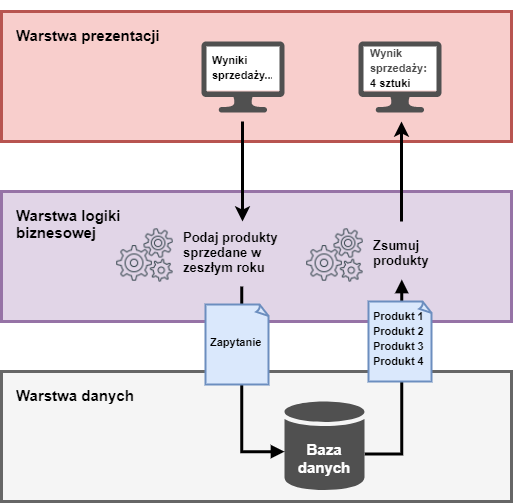
\includegraphics[width=0.7\linewidth]{graphics/chapter-3/three-tier-architecture.png}
	\caption{Ogólna architektura aplikacji trójwarstwowej}
	\label{three-tier-architecture}
\end{figure}

 
\noindent Istnieją oczywiście architektury posiadające więcej warstw, jednak są one mało popularne i~budowane specjalnie na potrzeby specyficznych i bardzo wymagających projektów.


\section{Warstwa prezentacji - aplikacja kliencka}
\quad W ramach implementacji warstwy aplikacji zdecydowano się skorzystać z jednego z bardzo popularnych w ostatnich latach \textit{frameworków javascriptowych}, które dedykowane są do obsługi i komunikacji z klientem. Środowisko bibliotek \textit{javascriptowych} jest obecnie bardzo szybko rozwijającym się elementem i istnieje wiele, różnego rodzaju rozwiązań tego typu. Najlepiej obecne trendy przedstawiają wykresy generowane przez system \textit{Google Trends} pokazujące popularność odpowiednich fraz w określonym przedziale czasowym. Poniżej znajduje się właśnie jeden z takich wykresów. Porównuje on zainteresowanie użytkowników sieci czterema najpopularniejszymi bibliotekami. W ramach wyjaśnienia wartości prezentowanych na osiach wykresu warto jest przytoczyć krótki tekst z instrukcji obsługi tego narzędzia:\\
\begin{quote}
    \item,,Liczby przedstawiają, jak często hasło było wyszukiwane w odniesieniu do najwyższego punktu wykresu w danym czasie i regionie. Wartość 100 oznacza najwyższą popularność hasła. Wartość 50 oznacza, że popularność hasła była dwukrotnie mniejsza. Natomiast 0~świadczy o tym, że popularność hasła wynosiła mniej niż 1\% najwyższej wartości \cite{google-trends}.'' 
\end{quote}

\begin{figure}[ht]
	\centering
	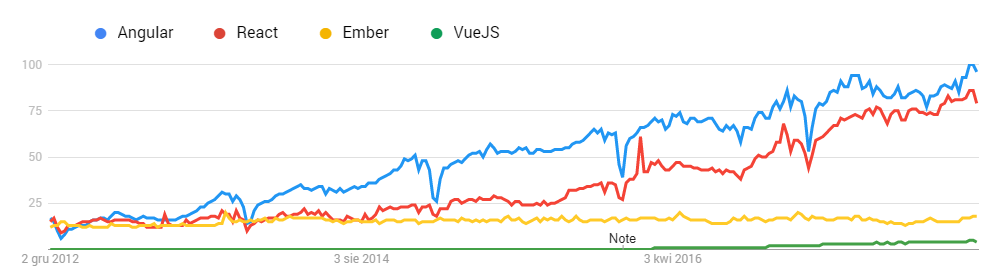
\includegraphics[width=1\linewidth]{graphics/chapter-3/frontend-frameworks.png}
	\caption{Porównanie popularności \textit{frameworków} aplikacji klienckich \cite{google-trends}}
	\label{fig:frontend-frameworks}
\end{figure}
\noindent Z przedstawionego wykresu jasno wynika, iż największym zainteresowaniem, deklasując przy tym konkurencję, cieszą się dwa rozwiązania: \textit{Angular} oraz \textit{React}, między którymi istnieje kilka zasadniczych różnic, takich jak np.: sposób wiązania danych (\textit{ang. data binding}), obsługa \textit{DOM}, czy sam fakt, że \textit{Angular} jest pełnoprawnym frameworkiem, natomiast \textit{React} jedynie biblioteką języka \textit{JavaScript} \cite{angular-react-comparison}. Ze względu, na fakt ukierunkowania Angular'a na programowanie obiektowe (\textit{ang. Object Oriented Programming - OOP}), lepszą dokumentację oraz większą ilość materiałów naukowych, a także doświadczenie w praktycznym wykorzystaniu, zdecydowano się wybrać właśnie tę technologię.



\subsection{Framework Angular}

\quad Jest to nowoczesny i otwarty \textit{frontendowy framework} oparty na języku \textbf{\textit{TypeScirpt}}, którego twórcą jest firma \textit{Google}. Głównym zadaniem biblioteki jest wdrożenie wzorca \textit{\textbf{serwis - kontroler}} w celu ułatwienia konstruowania i rozwoju aplikacji internetowych. \\
\\
Pierwsza wersja biblioteki powstała pod nazwą \textit{Angular} w roku 2009. Framework zyskał dużą popularność i przeszedł ogromną metamorfozę w stosunkowo krótkim czasie. Szybkie pojawianie się kolejnych wersji wymusiło konieczność usystematyzowania nazewnictwa. W~ten sposób pierwsza wersja \textit{Angular'a} zmieniła nazwę na \textit{AngularJS}, natomiast kolejna, która pojawiła się 22 listopada 2014 roku i wprowadziła drastyczne zmiany w strukturze biblioteki przyjęła nazwę \textit{Angular 2.0}. Następna, wersja 4.0, pojawiła się 13 grudnia 2016 i przyniosła już o wiele mniej zmian i nowości w stosunku do różnic między wersją \textit{JS}, a~\textit{2.0}. W momencie rozpoczynania projektu była to najnowsza wersja tej biblioteki (dokładnie \textit{4.4.6}), jednakże już 1 listopada 2017 roku pojawiła się wersja określona numerem \textit{5.0.0}, a kolejne wersje \textit{6} i~\textit{7} planowane są na okres najbliższego roku. Mówiąc o ogromnej zmianie między wersjami \textit{JS}, a \textit{2.0} należy wspomnieć przede wszystkim o: różnicy w implementowanych wzorcach projektowych - \textit{AngularJS} oparty o wzorzec model-widok-kontroler (\textit{MVC}), natomiast wersja 2.0 o model serwis-kontroler. Zmiana wzorca projektowego uniemożliwia wykonanie aktualizacji aplikacji z wersji \textit{JS} na \textit{2.0}, gdyż operacja taka wymagałaby napisania całej architektury całkowicie od początku. Drugą różnicą jest wykorzystany do implementacji język \textit{Javascript} w wersji pierwszej, natomiast w wersji drugiej - \textit{Typescript}, który jest nadzbiorem \textit{Javascriptu} wspierającego budowę przejrzystszego i bardziej uporządkowanego kodu. Pomniejszych zmian i różnic między wersją \textit{JS}, \textit{2.0} i \textit{4.0} (a nawet \textit{5.0}) jest o wiele więcej i~~warto zapoznać się w tej kwestii z doskonałym zestawieniem autorstwa firmy \textit{Angular Minds} \cite{angular-comparison}.\\
\\
Stopniowe zdobywanie popularności coraz to nowszych wersji biblioteki \textit{Angular} doskonale prezentuje kolejny wykres zapożyczony z serwisu \textit{Google Trends} przedstawiający zainteresowanie użytkowników wyszukiwarki \textit{Google} konkretnymi frazami:
\begin{figure}[ht]
	\centering
	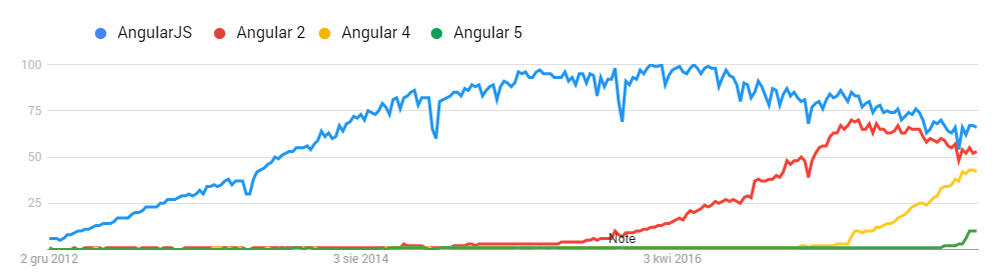
\includegraphics[width=1\linewidth]{graphics/chapter-3/angular-frameworks.png}
	\caption{Porównanie popularności wersji \textit{Angular'a} \cite{google-trends}}
	\label{fig:angular-version-comparison}
\end{figure}

\noindent W ramach wdrożenia projektu zdecydowano się na najnowszą dostępną wówczas wersję \textit{Angular'a} tj. \textit{4.4.6} umożliwiającego szybkie budowanie aplikacji typu \textit{single page}. Korzyści i~możliwości jakie daje wykorzystanie tej technologii to:
\begin{itemize}
    \item Łatwość stworzenia i rozwijania projektu dzięki konsolowemu narzędziu \textbf{\textit{Angular CLI}}.
    \item Mimo stosunkowo dużego rozmiaru samej biblioteki (w porównania z konkurencyjnymi rozwiązaniami), duża wydajność działania i wiele modułów dostępnych domyślnie - bez konieczność ich dodatkowej instalacji.
    \item Dwukierunkowe wiązanie danych (\textit{ang. Two way data binding}) zapewniające automatyczną aktualizację danych modelu.
    \item Architektura i podział całego projektu na moduły ułatwiający utrzymanie kodu i tworzenie go zgodnie z regułą \textbf{\textit{DRY}} (\textit{ang. Don't repeat yourself}).
    \item Wiele wbudowanych dyrektyw skracających czas wykonywania i tworzenia podstawowych zadań.
    \item Bardzo dobra obsługa formularzy i ich walidacji ułatwiająca tworzenie aplikacji nastawionych na częste interakcje z użytkownikiem.
\end{itemize}
Ogólny zarys przepływu danych w aplikacji wygląda w ten sposób, iż głównym elementem aplikacji opartej o \textit{Angular} jest \textbf{moduł}. Każda aplikacja ma przynajmniej jedną klasę modułu, który jest modułem głównym i umownie nazywany jest \textit{AppModule}. Moduły opierają się o \textbf{szablony} (\textit{ang. templates}) połączone ze znacznikami \textit{Angular'a}. Do zarządzania szablonami tworzone są klasy \textbf{komponentów}, do których \textbf{wstrzykiwane są zależności} (\textit{ang. dependency injection}) zawierające logikę aplikacji w postaci \textbf{serwisów} (\textit{ang. services}). \textit{Angular} generuje i przetwarza strukturę dokumentu DOM zgodnie z instrukcjami reprezentowanymi przez \textbf{dyrektywy}.  Ostatnim kluczowym elementem są \textbf{metadane}, które informują \textit{Angular'a}, iż dany element jest np. komponentem lub dyrektywą. Graficzne przedstawienie architektury \textit{Angular'a} przedstawia \textit{rysunek 3.4}.

\begin{figure}[ht]
	\centering
	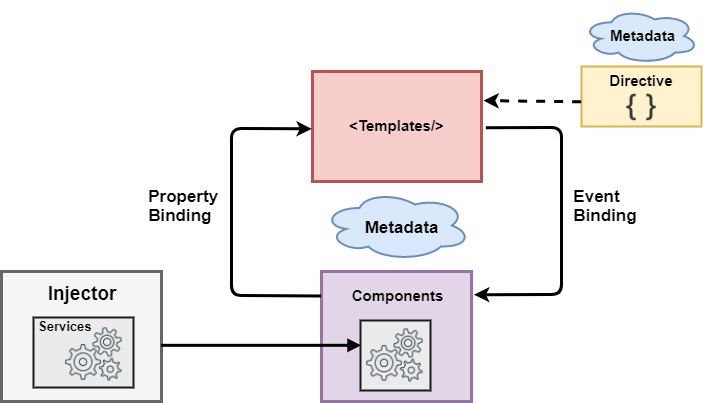
\includegraphics[width=1\linewidth]{graphics/chapter-3/angular-architecture.png}
	\caption{Ogólna architektura \textit{frameworka Angular 4}}
	\label{fig:general-angular-architecture}
\end{figure}

	\subsubsection{Angular CLI}
\quad Wspomniane już wcześniej, jako jedna z licznych zalet \textit{Angular'a}, narzędzie \textbf{\textit{Angular CLI}} to konsolowy interfejs służący do budowania, utrzymania, rozwijania i konfigurowania aplikacji stworzonych właśnie w tej technologii. W ostatnim czasie stało się jednym z najczęściej wykorzystywanych narzędzi do tego typu zadań. 
Usprawnia ono proces budowania nowego projektu ograniczając konieczność wykonania wielu niełatwych i powtarzalnych czynności do jednej konsolowej komendy. Przykładem może być polecenie tworzące nowy projekt:

\vspace{2mm}

    \centerline{\texttt{\hl{ ng new [name] }}}

\vspace{2mm}

\noindent Po wykonaniu tej komendy zostaje wygenerowany podstawowy szablon, który jest gotowy do uruchomienia za pomocą komendy:

\vspace{2mm}

    \centerline{\texttt{\hl{ ng serve }}}

\vspace{2mm}

\noindent Dzięki tym dwóm prostym komendom został stworzony i uruchomiony w pełni funkcjonalny projekt aplikacji, oszczędzając w ten sposób programiście kilku godzin żmudnych ustawień i~konfiguracji.\\
\textit{Angular CLI} nie ogranicza się jednak jedynie do generowania projektu. Jest również bardzo przydatne w czasie jego rozwoju, np. przy pomocy jednej komendy generując wszystkie potrzebne pliki dla nowego komponentu czy modułu:

\vspace{2mm}

    \centerline{\texttt{\hl{ ng generate component [name] }}}
    \centerline{\texttt{\hl{ ng generate module [name] }}}

\vspace{2mm}


	\subsubsection{Komponent ng2-file-upload}
	\quad Omawiając wszystkie ważne składowe aplikacji klienckiej, koniecznie należy wspomnieć o~jednym z komponentów, który ma zostać wykorzystany w aplikacji \textit{PhotoLab}.\\
	\textbf{\textit{Ng2-file-upload}} jest doskonałym przykładem jednego z bardzo wielu gotowych i ogólnodostępnych komponentów (na odpowiedniej licencji: np. \textit{MIT}) dedykowanych dla \textit{frameworka Angular}. Ogromna ilość komponentów wskazuje na wspominane wcześniej bardzo szeroko rozwinięte \textit{community}. Posiadanie grona takich osób dla każdej technologii jest bardzo ważne, gdyż gwarantuje: 
	\begin{itemize}
	    \item Szerokie wsparcie w przypadku problemów - programiści oferują wzajemną pomoc w~rozwiązywaniu problemów i dzielą się własnym doświadczeniem.
	    \item Ogromną ilość materiałów, poradników i szkoleń dostępnych w Internecie, które pozwalają w przyjazny sposób zaznajomić się z konkretnymi zagadnieniami.
	    \item Szybki rozwój (w przypadku \textit{Angular'a} jest bardzo dobrze widoczne) i aktualność z panującymi trendami, a wręcz bycie ich prekursorem.
	\end{itemize}
	\textit{Ng2-file-upload} to stworzony przez jednego z członków społeczności i udostępniony na licencji \textit{MIT} komponent odpowiedzialny za obsługę wgrywania plików. Oferuje on bardzo przystępny interfejs użytkownika z uwzględnieniem takich elementów jak:
	\begin{itemize}
	    \item Wybór plików za pomocą standardowego okna systemowego lub zasady przeciągnij i~upuść (\textit{ang. drag and drop}).
	    \item Wypisanie wybranych plików gotowych do wgrywania.
	    \item Możliwość wgrywania wszystkich wybranych plików jednocześnie.
	    \item Animowany pasek postępu procesu przesyłania.
	\end{itemize}
	Aby system ten sprostał wymaganiom \textit{PhotoLab} wystarczy wprowadzić do niego kilka modyfikacji takich jak np.: dołączenie podglądu wybranych zdjęć, czy ograniczenie opcji przesyłania plików jedynie do wszystkich jednocześnie. Należy również zaznaczyć, iż komponent ten działa jedynie w warstwie prezentacji, co oznacza, iż konieczne jest zaimplementowanie obsługi uzyskanych informacji (czyli zapisanie plików i informacji o nich) po stronie serwera aplikacji.
	% Komponent umożliwiający obsługę dynamicznego wgrywania zdjęć

\subsection{Bootstrap}
\quad Warstwa aplikacji to nie tylko interfejs przysyłający dane do kolejnej warstwy. To również, a wręcz przede wszystkim interakcja z użytkownikiem systemu, który chce skorzystać z usług firmy. Bardzo ważnym aspektem jest więc zaprezentowanie danych i funkcjonalności w sposób estetyczny, usystematyzowany i przyjazny dla człowieka. Do tego celu służą właśnie kaskadowe arkusze stylów (\textit{ang. Cascading Style Sheets (CSS)}), które opisują formę prezentacji struktury utworzonej w hipertekstowym języku znaczników (\textit{ang. HyperText Markup Language}), czyli popularnym \textit{HTML'u}. Czasy, gdy całe strony i duże aplikacje internetowe były dekorowane jedynie przy pomocy czystego \textit{CSS} dawno minęły. Obecnie na szeroką skalę wykorzystuje się \textbf{\textit{frameworki CSS}}, czyli biblioteki zawierające zestaw wielu gotowych narzędzi i komponentów ułatwiających tworzenie estetycznych i przejrzystych interfejsów stron internetowych. \\
\\
Jednym z takich rozwiązań jest \textbf{\textit{Bootstrap}}. Jest to obecnie, podobnie jak \textit{Angular}, najpopularniejsze i najszerzej wykorzystywane narzędzie w swojej klasie charakteryzujące się bardzo prężnym rozwojem. Zespołem odpowiedzialnym za \textit{Bootstrap'a} są programiści \textit{Twitter'a}. 10 sierpnia 2017 roku opublikowali oni najnowszą wersję \textit{4.0.0 beta 2}, która to właśnie wersja zostanie wdrożona w aplikacji \textit{PhotoLab}. Argumentami za zastosowaniem technologii znajdującej się jeszcze w wersji beta była przede wszystkim jej bardzo dobra stabilność (jak na wersję beta), szerokie grono społeczności, dobra dokumentacja, a przede wszystkim różnice względem poprzedniej wersji (\textit{3.3.7}):
\begin{itemize}
    \item pliki źródłowe tworzone w technologi \textit{SASS}, a nie \textit{LESS},
    \item domyślna jednostka, \textit{rem} - czyli wysokość czcionki elementu korzenia w drzewie dokumentu, a nie piksel,
    \item pięcio-, a nie czterowarstwowy \textit{grid}, czyli siatka, według której budowany jest szablon,
    \item wbudowany nowy sposobu układania elementów na stronie - \textit{FlexBox}.
\end{itemize}
Powodem wyboru \textit{Bootstrap'a} jako \textit{frameworka CSS} jest jego dobra znajomość i doświadczenie w wykorzystaniu, co znacznie ułatwi i przyspieszy pracę nad aplikacją ale przede wszystkim bardzo estetyczny sposób prezentowania treści w formie, która w pełni zadowala właściciela laboratorium.

\section{Warstwa logiki biznesowej - serwer aplikacji}

\quad Bardzo ważną częścią przygotowywania projektu jest podjęcie decyzji o wyborze technologii dla warstwy aplikacji, czyli warstwy najważniejszej dla całego modelu trójwarstwowego. W tej płaszczyźnie bowiem wykonywane są najistotniejsze operacje obsługujące procesy biznesowe, takie jak wyliczenia, autoryzacja użytkowników czy dostęp do danych. Podejmując decyzje należy mieć na względzie postawione cele tj. bezpieczeństwo aplikacji, jej wydajność i dostępność oraz możliwie niskie koszty wdrożenia i utrzymania. \\
\\
Możliwości i technologii jest wiele. Jedne są bardziej odpowiednie, inne mniej. Ścisła czołówka tzw. \textit{aplikacji backendowych} to z pewnością technologie takie jak: \textit{PHP}, \textit{.NET} i~\textit{Java}, jednak coraz większą popularność zyskują również: \textit{Python} czy \textit{Ruby}.\\
Wybór nie jest łatwy. Żadne wskaźniki wydajności, takie jak szybkość, wydajność, czy bezpieczeństwo, nie wskazują konkretnego faworyta tej konkurencji. Wybór technologi, w której zostanie zaimplementowana aplikacja został więc wybranych w oparciu o aspekt wewnętrzny jakim są predyspozycje autora. W ramach implementacji warstwy biznesowej aplikacji \textit{PhotoLab} wykorzystana zostanie technologia \textbf{\textit{ASP.NET Core}}.

\subsection{ASP.NET Core}
\quad \textbf{\textit{.NET Framework}} jest to platforma programistyczna wywodząca się z rodziny rozwiązań firmy \textit{Microsoft}.  Dostarcza wiele standardowych funkcjonalności w postaci \textbf{bibliotek klas} oraz przede wszystkim \textbf{środowisko uruchomieniowe} (\textit{ang. Common Language Runtime} (\textit{CLR}). \\
Technologia ta nie jest związana z żadnym konkretnym językiem programowania i umożliwia budowanie kodu w oparciu o jeden z bardzo wielu dostępnych, m.in. \textit{C++}, \textit{C\#} czy \textit{F\#}. Platforma \textit{\textbf{ASP.NET}} to, podobnie jak \textit{ADO.NET} (używana jako narzędzie dostępu do danych), pochodna platformy \textit{.NET} służąca do budowania dynamicznych strony WWW. \\
    \textbf{\textit{ASP.NET Core}} jest biblioteką aplikacji internetowych, który wchodząc na rynek w połowie 2016 roku w wersji \textit{1.0} wprowadził ogromną rewolucję w produktach z serii \textit{ASP.NET}: 
    \begin{enumerate}
        \item Zintegrował wszystkie trzy osobno występujące modele aplikacji internetowych, czyli:
    \begin{itemize}
        \item \textit{ASP.NET MVC} - bibliotekę implementującą wzorzec \textit{Model-View-Controller} (\textit{MVC}) w aplikacjach internetowych.
        \item \textit{ASP.NET Web API} - strukturę typu \textit{HTTP API} służącą do budowania \textit{web serwisów}.
        \item \textit{ASP.NET Web Pages} - platformę wykorzystującą jedynie strony oparte o  składnię \textit{Razor}.
    \end{itemize}
   \item Został całkowicie przebudowany i stworzony w zupełnie nowym stosie technologicznym, zachowując przy tym jednak bardzo duże podobieństwo konceptualne z \textit{ASP.NET MVC}.
    \item Jego całkowite przebudowanie umożliwiło:
        \begin{itemize}
            \item stworzenie wieloplatformowej technologii dostępnej już nie tylko na systemy \textit{Windows}, ale również \textit{Linux} i \textit{Mac},
            \item zbudowanie modularnej biblioteki opartej o paczki \textit{NuGet'owe},
            \item udostępnienie oprogramowania na otwartej licencji \textit{MIT}, która nakierowana jest na rozwój społecznościowy,
            \item zunifikowanie sposobu generowania interfejsów internetowych,
            \item całkowite przyspieszenie działania całej platformy względem jej poprzednich wersji,
            \item stworzenie nowego, bardzo lekkiego i modułowego potoku żądań HTTP (\textit{ang. request pipeline}).
        \end{itemize}
    \end{enumerate}
    Kierując się wszystkimi wspomnianymi powyżej przesłankami, została podjęta decyzja o~wdrożeniu projektu aplikacji internetowej (ASP.NET Core Web Application) o strukturze typu \textbf{\textit{Web API}} w najnowszej obecnie wersji \textbf{\textit{1.1}}.\\
    \\
    Poniżej (\textit{rys. 3.5}) przedstawiony został ogólny zarys
    obsługi żądań zapytań \textit{HTTP} docierających do warstwy biznesowej aplikacji opartej o technologię \textit{ASP.NET Core Web API} i~obsługującej połączenie z bazą danych poprzez narzędzie \textit{Entity Framework}.

    \begin{figure}[ht]
	\centering
	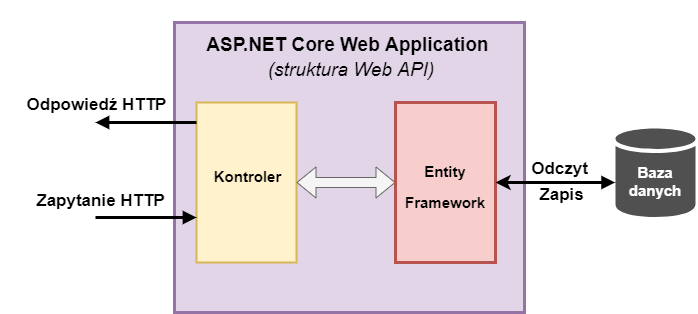
\includegraphics[width=1\linewidth]{graphics/chapter-3/asp-net-web-api-architecture.png}
	\caption{Architektura i przepływ danych warstwy biznesowej}
	\label{fig:asp-net-web-api-architecture}
    \end{figure}

\subsection{ASP Identity i JSON Web Token}
\quad W celu zapewnienia zakładanego, wysokiego poziomu bezpieczeństwa zarówno klientów systemu jak i przechowywanych w nim danych, konieczne jest zaimplementowanie systemu weryfikującego użytkowników. Zanim jednak zostanie omówione wybrane rozwiązanie należy wyjaśnić kilka pojęć związanych z tą tematyką.\\
    \\
    Z kwestią bezpieczeństwa nierozerwalnie związane są trzy pojęcia, które często są mylone i niepoprawnie definiowane. Istnieje wiele definicji i wywodów na temat każdego z~poniższych haseł, jednak najprostsze wyjaśnienia przedstawiają się następująco:
    \begin{itemize}
        \item \textbf{Identyfikacja} (\textit{ang. identity}) - rozpoznanie użytkownika, próbującego połączyć się z systemem.
        \item \textbf{Uwierzytelnienie} (\textit{ang. authentication}) - upewnienie co najmniej jednej ze stron o tożsamości drugiej. Jest to tak naprawdę identyfikacja na poziomie zaawansowania i szczegółowości pozwalającej na przyznanie odpowiednich uprawnień i dostępów.
        \item \textbf{Autoryzacja} (\textit{ang. authorization}) - jest to zapewnienie stronie zgłaszającej taką potrzebę odpowiednich uprawnień i praw dostępu. 
    \end{itemize}
    Podsumowując: ,,identyfikacja, uwierzytelnianie i autoryzacja powinny być elementami każdej transakcji biznesowej i muszą być zagwarantowane przez system komunikacyjny i oprogramowanie pośredniczące w związkach pomiędzy dostawcami i klientami \cite{identity-theory}''. \\
    \\
    Cały system weryfikacji użytkowników można zaimplementować samodzielnie od podstaw. Mija się to jednakże z celem w momencie, gdy platforma \textit{.NET} udostępnia świetne narzędzie jakim jest \textbf{\textit{ASP.NET Identity}}. Dlaczego warto wybrać akurat to, gotowe rozwiązanie? Z pewnością dlatego, iż cały system weryfikacji użytkowników jest procesem trudnym i skomplikowanym, a najmniejsza luka w jego implementacji powoduje pojawienie się tzw. najsłabszego ogniwa, które powoduje, iż inne, nawet najmocniejsze zabezpieczenia tracą swoją wartość. \textit{ASP.NET Identity} jest produktem rozwijanym i modyfikowanym od wielu lat, uwzględniane są w nim wszystkie najnowsze mechanizmy, zabezpieczenia, sugestie użytkowników oraz dostrzeżone błędy i uchybienia. Gotowy system, stworzony przez duży zespół wsparty ogromnym \textit{community}, wykorzystany i przetestowany na setkach tysięcy rozwiązań i systemów, zarówno mniejszych, jak i większych, jest idealnym wyborem dla zapewnienia bezpieczeństwa aplikacji \textit{PhotoLab}.\\
    \\
    Mimo wielu zalet, dostrzeżono również dwa poważne mankamenty tego rozwiązania. Biblioteka ta działania jedynie w drugiej warstwie modelu - warstwie biznesowej. Oznacza to, iż sesje zalogowanego użytkownika muszą być przetrzymywane na serwerze, co powoduje jego dodatkowe obciążenie. Drugi przypadek zakłada dalszy rozwój aplikacji i pojawienie się dodatkowych serwisów, np. do obsługi urządzeń mobilnych. W takim przypadku konieczna jest ponowna implementacja systemu weryfikacji użytkownika na kolejnym serwerze i przez to redundancja kodu i odpowiedzialność. Rozwiązaniem tego typu problemów jest uzupełnienie biblioteki \textit{ASP.NET Identity} o standard kluczy dostępu \textbf{\textit{JSON Web Token}}.\\
    Jest to otwarta technika generowania kluczy uwzględniających prawa dostępu. Zasada jej działania oparta jest na zasadzie klucza prywatnego. Niepowtarzalny klucz JWT generowany jest w momencie logowania użytkownika i składa się z trzech części:
    \begin{itemize}
        \item \textbf{nagłówka} (\textit{ang. header}) - zawierającego informacje o typie \textit{klucza JWT} oraz sposobie jego szyfrowania,
        \item \textbf{ładunku} (\textit{ang. payload}) - jak sama nazwa wskazuje, przechowującego informacje na temat praw dostępów, czy np. czasu ważności tokenu,
        \item \textbf{podpisu} (\textit{ang. signature}) - do którego utworzenia konieczne są dwie pozostałe części, które zabezpieczone są poprzez sekretny klucz aplikacji i szyfr ustalony w nagłówku.
    \end{itemize}
    Klucz generowany jest po stronie serwera aplikacji i zwracany do warstwy klienckiej, w której może być przetrzymywany, np. w pamięci lokalnej. W momencie odwołania się użytkownika do zabezpieczonej warstwy biznesowej, wraz z zapytaniem przesyła on \textit{klucz JWT}, który jest jedynie weryfikowany i w razie sukcesu otwiera dostęp do zasobów / funkcjonalności lub w~razie niepowodzenia serwer zwraca odpowiedź z kodem błędu 403.\\
\\
Zastosowanie \textit{kluczy JWT} rozwiązuje dwa wcześniej wymienione problemy pojawiające się w momencie korzystania z modułu \textit{Identity}. Po pierwsze ciężar zapamiętania sesji logowania przerzuca na aplikację kliencką, odciążając w te sposób serwer, który nie musi już przetrzymywać w swojej pamięci bazy zalogowanych użytkowników. Po drugie mechanizm autoryzacji może zostać zaimplementowany na jednym z obsługujących aplikację serwerów, do którego użytkownik zawsze będzie się odnosił wyłącznie w momencie logowania. Pozostałe moduły będą musiały jedynie sprawdzić poprawność otrzymanego klucza i udostępnić swoje zasoby. Opisaną sytuację doskonale przedstawia diagram (\textit{rys. 3.6}):
    
    
    \begin{figure}[ht]
	\centering
	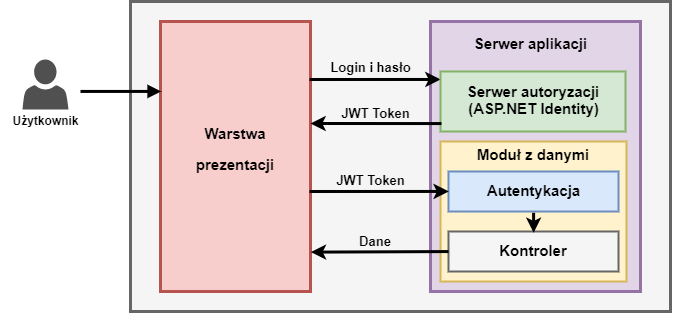
\includegraphics[width=1\linewidth]{graphics/chapter-3/jwt-identity-diagram.png}
	\caption{Weryfikacja użytkownika z użyciem \textit{ASP.NET Identity} i \textit{JSON Web Token}}
	\label{fig:jwt-identity-diagram}
    \end{figure}




\section{Warstwa danych - baza danych}
\quad Ostatnim elementem modelu trójwarstwowego aplikacji jest warstwa danych.
    Najczęściej można ją opisać jako swoisty pojemnik na informacje. Powinien on zapewniać bezpieczeństwo i trwałość swojej zawartości oraz łatwą i szybką jej dostępność. \\
    \\
    Istnieje obecnie wiele rodzajów baz danych, które różnią się względem siebie sposobem przetrzymywania informacji. Wybrane z nich to bazy:
    \begin{itemize}
        \item \textbf{Proste} (kartotekowe) - tablica danych skonstruowana jest jako samodzielny dokument, który nie może wchodzić w związki z innymi tablicami. Przykładami implementacji takiej bazy mogą być: książki telefoniczne, książki kucharskie czy różnego rodzaju spisy.
        \item \textbf{Relacyjne} (\textit{RDB}) - dane przetrzymywane w postaci encji umieszczonych w tabelach, które z kolei mogą wchodzi w relacje między sobą. Posiadają predefiniowane typy oraz wewnętrzne języki programowania (\textit{SQL}). Przykładami są bazy: \textit{Oracle}, \textit{Ingress}, \textit{Access}, \textit{\textit{MySQL}} czy \textit{MS SQL}. Obecnie dominujący typ danych w zastosowaniach komercyjnych (ok. 95\% rynku).
        \item \textbf{Obiektowe} (\textit{ODB}) - nie zdefiniowane żadnym oficjalnym standardem. Ich podstawowym zadaniem jest odwzorowanie obiektów i powiązań wchodzących w skład aplikacji na identyczne w bazie danych. Łączą one właściwości obiektowości i obiektowych języków programowania wraz z możliwościami systemów bazodanowych.
        \item \textbf{Nierelacyjne} (\textit{NoSQL}) - nie posiadają ściśle zdefiniowanej struktury. Dane składowane jako dokumenty - np. w formie \textit{JSON}. Charakteryzują się dużą skalowalnością i wydajnością. Przykładamy implementacji tego typu baz są: \textit{MongoDB} oraz \textit{Apache Cassandra}.
    \end{itemize}
    Najbardziej naturalnym i najczęstszym wyborem w przypadku konstruowania warstwy pośredniej w technologii \textit{ASP.NET} jest zbudowanie środowiska bazodanowego w oparciu o produkt pochodzący z tej samej rodziny - firmy Microsoft - jakim jest \textbf{\textit{Microsoft SQL Server}}. Połączenie, dodatkowo wzbogacone o narzędzie klasy \textbf{\textit{ORM}} - \textit{\textbf{Entity Framework}} - stawowi doskonały pakiet zapewniający najlepsze możliwe połączenie warstwy aplikacji i warstwy danych modelu trójwarstwowego.\\
    \\
    Wykorzystanie relacyjnej bazy danych daje wszystkie możliwe korzyści wynikające z przechowywania danych w takiej strukturze tj.: możliwość stosowania złożonych kryteriów wyszukiwania, bardzo dobre mechanizmy dostępu do danych, a także pewną i sprawdzoną strukturę przetestowaną w wielu możliwych scenariuszach i przypadkach. Nie jest być może to struktura najszybsza, ani najbardziej podatna na skalowalność, jednakże w aplikacji \textit{PhotoLab} nie są to kryteria najważniejsze. Bardzo dużą zaletą i ułatwieniem w operowaniu na bazie relacyjnej typu \textit{MS SQL}, gdzie reprezentacja danych nie zawsze jest przyjazna i naturalna, jest narzędzie służące do mapowania obiektowo-relacyjnego. Zdecydowania ułatwia to pracę nad aplikacją oraz przyspiesza jej rozwój. Wykorzystując narzędzia typu \textit{ORM}, czasami mogą pojawiać się problemy wydajnościowe, jednak w przypadku projektowanej aplikacji nie przewiduje się takowych, tak więc liczba zalet zdecydowanie przewyższa wady wprowadzenia tego rozwiązania.
    
\subsection{Microsoft SQL Server}
\quad System służący do zarządzania bazą danych, którego twórcą jest firma \textit{Microsoft}. Jest to flagowy produkt tej korporacji w zakresie operacyjnych systemów zarządzania bazami danych (\textit{ang. Operational Database Management Systems (ODBMS)}.\\
    \\
    Podstawą platformy \textit{SQL Server} jest usługa serwera (\textit{ang. database engine}), który realizuje wszystkie zadania dotyczące obsługi i utrzymania bazy danych. Całe środowisko \textit{SQL Server} jest skalowalne, w zależności od potrzeb i wymagań może składać się z wielu różnych komponentów. Na jednym serwerze (fizycznym, bądź wirtualnym)  możliwa jest instalacja wielu \textit{instancji} środowiska \textit{SQL Server}. Ta z kolei może zarządzać wieloma \textit{bazami danych}. Zazwyczaj jednak poprzez względy wydajnościowe na jednym serwerze instaluje się jedną instancję z maksymalnie dwoma lub trzema bazami danych.\\
    \\
    Kilka najbardziej podstawowych i oferowanych przez \textit{SQL Serwer} komponentów to:
    \begin{itemize}
        \item Wspomniany wcześniej \textbf{silnik bazy danych}.
        \item \textbf{Usługi raportujące} jako gotowy system oparty o technologię \textit{.NET} do generowania raportów z bazy danych.
        \item \textbf{Usługi analityczne} w skład których wchodzi kilka narzędzie analitycznych głównie z zakresu \textit{Business Intelligence}, czyli przetwarzania danych w informacje, by następnie wyciągnąć z nich odpowiednie wnioski i wiedzę.
        \item \textbf{Usługi integracji danych} oferujące możliwość zbierania i analizy danych z różnych źródeł. 
    \end{itemize}
    Omawiając pakiet bazodanowy \textit{Microsoft} należy również wspomnieć o udostępnionych w ramach niego narzędziach takich jak: \textbf{\textit{SQL Server Profiler}} i \textbf{\textit{SQL Server Management Studio}}. Drugie przedstawione narzędzie zostanie wykorzystane w ramach wdrożenia projektu w celu: administracji, przeglądu i edycji danych w graficznym środowisku użytkownika (\textit{GUI}).
    
    \subsection{Entity Framework Core}
\quad Entity Framework podobnie jak \textit{SQL Server Management Studio} należy do technologii z~rodziny \textit{.NET}, a konkretnie \textit{ADO.NET}, a więc jest doskonale zintegrowane do obsługi bazy danych \textit{Microsoft SQL} oraz aplikacji \textit{ASP.NET}.
    \\
    \\
    Jest to narzędzie typu \textbf{ORM} (\textit{ang. Object-relational mapping}), czyli takie, które odwzorowuje obiekty architektury obiektowej na tabele i encje w relacyjnej bazie danych. Odwzorowanie takie ma bardzo dobre zastosowanie w przypadku tworzenia systemu zorientowanego na podejście obiektowe, natomiast baza danych operuje na relacjach. Programiści w momencie zajmowania się danymi, mogą pracować na wyższym poziomie abstrakcji, przez co generują mniejszą ilość redundantnego kodu i ciągle pozostają w sferze programowania obiektowego, a~nie zorientowanego na tabele i encje.
\chapter{Projekt systemu}
{\em \quad Jest to rozdział, który przedstawia najważniejsze elementy systemu zarządzania laboratorium fotograficznym - \textit{PhotoLab}. Uwzględniono w nim omówienie struktury i logiki działania aplikacji oraz szczegółowe przyjrzenie się stronie serwerowej, jak i klienckiej. Pod koniec tej części dokumentacji zostanie przedstawiony proces instalacji aplikacji na serwerze produkcyjnym oraz krótka instrukcja jej użytkowania, zawierająca zrzuty ekranu najważniejszych elementów strony.}

\section{Struktura i logika działania aplikacji}
	
	\quad Tak jak zostało to nakreślone podczas ustalania szczegółów implementacyjnych aplikacji, została ona podzielona na 3 warstwy: aplikacji, serwerową i bazy danych. Użytkownicy strony internetowej mają dostęp jedynie do pierwszej z nich, opartej o \textit{framework Angular}. Ta z~kolei w celu przetworzenia zapytań użytkownika komunikuje się z serwerem aplikacji zbudowanym w postaci projektu \textit{ASP.NET Core Web API}, a on bezpośrednio z bazą danych \textit{Microsoft SQL Server}. Opisany ciąg działań świetnie obrazuje poniższy diagram:
	
	\begin{figure}[ht]
	\centering
	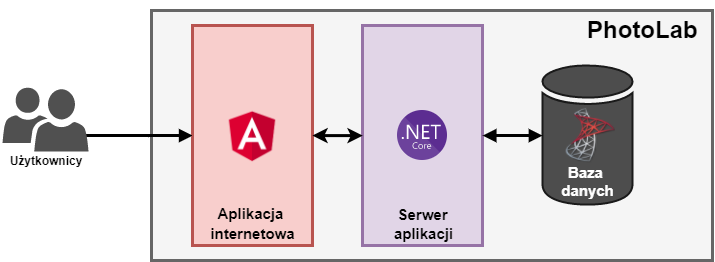
\includegraphics[width=1\linewidth]{graphics/chapter-4/general-application-architecture.png}
	\caption{Ogólny diagram architektury aplikacji \textit{PhotoLab}}
	\label{fig:general-application-architecture}
\end{figure}
\noindent Precyzując strukturę zademonstrowaną na rysunku \ref{fig:general-application-architecture}, należy poruszyć temat sposobu komunikacji między warstwami aplikacji i rodzajami użytkowników, którzy się z nią łączą.\\
	\\
	Temat użytkowników i ich dostępów zostanie poruszony szczegółowo w kolejnej sekcji. Na tym etapie wystarczy jedynie zaznaczyć, iż w systemie rozróżniane są trzy poziomy użytkowników: niezalogowany, zalogowany oraz administrator.\\
	\\
	Klient komunikuje się z aplikacją za pomocą licznych formularzy, przełączników i przycisków, natomiast serwis prezentuje żądane informacje w formie tekstowej, tabelarycznej oraz graficznie jako obrazy i wykresy.\\
	Przepływ danych pomiędzy warstwą kliencką, a serwerem aplikacji odbywa się poprzez zapytania (\textit{ang. request}) i odpowiedzi (\textit{ang. response}) \textit{HTTP} w postaci \textit{JSON}, czyli lekkiego formatu tekstowego bazującego na podzbiorze języka \textit{Javascript}.\\
	Wymiana danych serwera i bazy danych realizowana jest za pomocą tzw. \textit{ObjectModeli}, które są natywnym formatem obsługi wymiany informacji w  wykorzystywanym do tego narzędziu \textit{Entity Framework}. Uwzględniając dodatkowe informacje, można zmodyfikować poprzedni diagram do postaci przedstawionej na rysunku \ref{fig:application-architecture-without-payu}.
	
	
	
	
	\begin{figure}[ht]
	\centering
	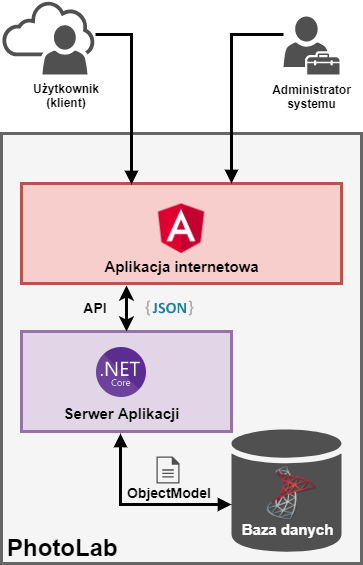
\includegraphics[width=0.5\linewidth]{graphics/chapter-4/application-architecture.png}
	\caption{Szczegółowy diagram architektury aplikacji \textit{PhotoLab}}
	\label{fig:application-architecture-without-payu}
\end{figure}
	
	
\noindent Głównym elementem, wokół którego operuje zasadnicza część aplikacji są \textbf{zlecenia}. To one umożliwiają złożenie zamówienia na wykonanie usługi, by następnie pracownik laboratorium na ich podstawie mógł wywołać odbitki oraz poinformować klienta o gotowym, oczekującym efekcie końcowym całego procesu. \\
	Każdemu etapowi zlecenia został przypisany odpowiedni stan, który jednoznacznie informuje zarówno klienta jak i pracownika zakładu o koniecznych do podjęcia krokach mających na celu zakończenie procesu sukcesem. Wszystkimi stanami zlecenia zarządza administrator systemu lub sam system czyni to automatycznie. Na poniższym diagramie został przedstawiony cykl życia zlecenia wraz z zaznaczonymi obszarami odpowiedzialności poszczególnych grup osób za zlecenie w danym stanie.
	
	\begin{figure}[ht]
    	\centering
    	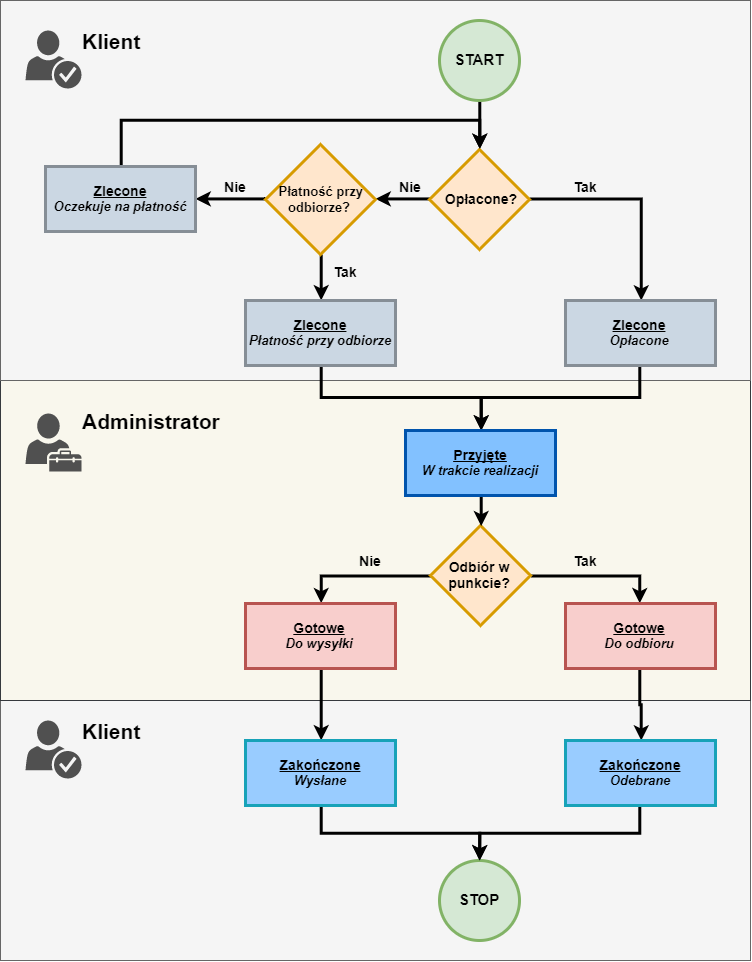
\includegraphics[width=0.9\linewidth]{graphics/chapter-4/order-states.png}
    	\caption{Cykl życia zlecenia}
    	\label{fig:order-states}
    \end{figure}
	
	\section{Dostęp i bezpieczeństwo}
	
\quad Serwis zapewnia zróżnicowany poziom dostępu na poziomie zarówno aplikacji internetowej, jak i serwera. Wyróżnione zostały \textbf{3 poziomy dostępu}:
	\begin{itemize}
	    \item \textbf{Użytkownik niezalogowany} - ma dostęp jedynie do podstawowych zasobów strony (głównie stron statycznych). Nie ma możliwości składania zleceń oraz dostępu do panelu administratora.
	    \item \textbf{Użytkownik zalogowany} - ma możliwość korzystania ze wszystkich użyteczności serwisu z modułu laboratorium. Brak możliwości zalogowania i użytkowania panelu administracyjnego.
	    \item \textbf{Administrator} - pełny dostęp do wszystkich możliwości serwisu.
	\end{itemize}
	
\noindent Po stronie \textit{Angular'a} ograniczenie dostępu odbywa się na poziomie \textit{routingu}, czyli wyznaczania ścieżki do podstron aplikacji. Służy do tego interfejs \textit{CanActivate} z paczki \textit{@angular/router}, który implementuje klasa ,,strażnika''.
	
\begin{listing}[ht]
    \jscode{listings/can-activate-interface.ts}
    \caption{Implementacja metody interfejsu \textit{CanActivate}}
    \label{listing:can-activate-interface}
\end{listing}

\noindent Tak stworzona klasa wstrzykiwana jest jako zależność do klasy odpowiedzialnej za sterowanie ruchem na stronie (\textit{router}), gdzie odpowiada za przydzielanie dostępu do odpowiedniej ścieżki adresu WWW.

\begin{listing}[ht]
    \jscode{listings/injection-auth-guard.ts}
    \caption{Wstrzyknięcie zależności \textit{AuthGuard} do klasy \textit{routing'u}}
    \label{listing:injection-auth-guard}
\end{listing}

\noindent Jak widać na powyższych listingach, w celu weryfikacji dostępu do danej sekcji strony sprawdzany jest status użytkownika (np. czy jest administratorem, lub czy jest zalogowany). Aby jednak aplikacja kliencka miała wiedzę dotyczącą przydzielonego poziomu dostępu, konieczna jest komunikacja z serwerem. Odbywa się to w momencie logowania do systemu - użytkownik wysyła dane logowania, system weryfikuje ich poprawność i zwraca odpowiedni \textit{Token JWT} wraz z informacjami o przydzielonych uprawnieniach.

\begin{listing}[ht]
    \cscode{listings/login-server.cs}
    \caption{Obsługa logowania użytkownika po stronie serwera}
    \label{listing:login-server}
\end{listing}

\noindent Tak otrzymaną odpowiedź należy jeszcze przetworzyć po stronie klienta. Służy do tego metoda \textit{login}, jednego ze stworzonych serwisów aplikacji (\textit{UserService}). W pierwszej kolejności wysyła ona zapytanie do serwera, które zostaje obsłużone przez metodę zaprezentowaną w~listingu powyżej. Następnie oczekuje na odpowiedź. Gdy takowa przyjdzie, należy ją obsłużyć. W przypadku aplikacji \textit{PhotoLab} jest to zapisanie \textit{tokena JWT} oraz identyfikatora użytkownika w lokalnej pamięci, ustawienie statusu jako \textit{,,zalogowany''} i ostatecznie zweryfikowanie, czy użytkownik posiada prawa administratora. 
\newpage
    
\begin{listing}[ht]
    \jscode{listings/login-client.ts}
    \caption{Obsługa logowania użytkownika po stronie klienta}
    \label{listing:login-client}
\end{listing}

\noindent Szczegółowe wyjaśnienie sposobu weryfikacji użytkownika za pomocą \textit{ASP.NET Identity} oraz standardu \textit{JWT Token} zostało zaprezentowane w rozdziale dotyczącym technologii warstwy logiki biznesowej (\textit{Rozdział 3.3.2}).\\
    Serwer aplikacji również posiada własny system weryfikacji dostępu użytkownika. Jest on zaimplementowany w postaci modułu \textit{ASP.NET Identity}, gdzie za poziom dostępu odpowiadają przydzielone użytkownikowi  prawa (\textit{ang. claims}). W momencie przekierowywania zapytania klienta do odpowiedniego kontrolera lub metody weryfikowane są prawa użytkownika (dostęp może być sprawdzany na jednym z dwóch lub na obu). Jeżeli zgłaszający zapytanie użytkownik posiada odpowiednie prawa, zapytanie jest realizowane. Jeżeli nie - zwracany jest błąd serwera w postaci kodu z numerem \textit{401} (\textit{Unauthorized}).
    
	\section{Serwer aplikacji i baza danych}
	
	\quad W sekcji tej zostanie omówiona architektura serwera aplikacji. Wyjaśnione zostaną kluczowe elementy tej warstwy wraz z przykładami w postaci listingu kodu. Poruszony zostanie również bardzo ważny temat bazy danych obsługującej cały serwis. Przedstawiona zostanie jej struktura, a także sposób komunikacji z serwisem.
	
\subsection{Struktura Web API}
\quad \textit{Web API} to bardzo ogólne pojęcie interfejsu korzystającego z protokołu \textit{HTTP} oraz formatu \textit{JSON} lub \textit{XML}. Pozwala na komunikowanie się użytkowników witryny z systemem aplikacji (serwerem) umieszczonym w dowolnej lokalizacji. \\
W przypadku aplikacji \textit{PhotoLab} została wdrożona implementacja  w postaci projektu \textit{ASP.NET Core Web API}. Ogólna struktura tego projektu przedstawiona została na rysunku \ref{fig:server-structure}.\\
Nie zagłębiając się w szczegółową budowę i strukturę projektu wygenerowanego przez oprogramowanie \textit{Visual Studio}, należy dostrzec jednak kilka kluczowych elementów serwera.

\begin{wrapfigure}[19]{l}{0.35\textwidth}
    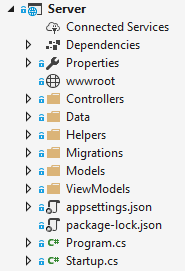
\includegraphics[width=1\linewidth]{graphics/chapter-4/server-structure.png}
    \caption{Struktura plików serwera aplikacji}
    \label{fig:server-structure}
\end{wrapfigure}

Najważniejsze z nich to foldery:
\begin{itemize}
    \item \textit{\textbf{Controllers}} - zbiór klas kontrolerów odpowiedzialnych za poszczególne działania, np. autentykację, użytkownika, obsługę zleceń czy statystyk serwisu. Kontroler jest klasą, która przechwytuje skierowane do niego zapytania \textit{HTTP}, przekazuje je do swojej odpowiedniej metody, która przetwarza informacje zgodnie z zaimplementowaną logiką, by następnie zwrócić je w postaci odpowiedzi \textit{HTTP}.
    \item \textit{\textbf{Data}} - zawiera klasę służącą do nawiązania połączenia z bazą danych.
    \item \textbf{\textit{Models}} - sekcja zawierają wszystkie modele obiektów, czyli reprezentantów informacji. Są one zbudowane jako klasy języka \textit{C\#}, zwane jako \textit{Plain Old C\# Object} (\textit{POCO}). Modele te, przekonwertowane przez \textit{Entity Framework} tworzą strukturę tabel bazy danych.
    \item \textbf{\textit{ViewModels}} - pakiet klas obiektów, nazywanych również \textit{DTO} (\textit{ang. Data Transfer Object}) służących do komunikacji serwera z aplikacją kliencką.
\end{itemize}

\noindent \textit{Web API} nie ma ustalonej i sztywno połączonej z nim aplikacji klienckiej. Dowolny serwis może nawiązać komunikację wykorzystując jedynie odpowiednie zapytania \textit{HTTP} skierowane pod ustalony adres. Z serwerem aplikacji \textit{PhotoLab} może łączyć się nie tylko specjalnie utworzony serwis oparty o \textit{Angular'a}, ale dowolny inny, np. nakierowany na działanie na urządzeniach mobilnych lub w przypadku testowania poprawności serwera (jak miało to miejsce w~czasie implementacji) - specjalnie przeznaczony do tego typu zabiegów program \textit{Postman}. 



\subsection{Baza danych}
\quad Ostatnią warstwą architektury trójwarstwowej jest baza danych. Serwis \textit{PhotoLab} to nie tylko wykonywane akcje, to również dane, na których operuje. Bez nich funkcjonowanie systemu byłoby niemożliwe. Większość działań podejmowanych na stronie odwołuje się do informacji przetrzymywanych właśnie w bazie danych. Znajdują się tam dane o~użytkownikach i~ich dostępach, złożonych zamówieniach, czy ustawieniach biznesowych (ceny, rodzaje papieru, możliwości wysyłki, płatności).\\
\\
Dzięki zastosowaniu narzędzia \textit{Entity Framework} i podejścia \textit{\textbf{Code First}} nie było konieczne tworzenie schematu bazy danych wprost \cite{entity-programming}. Podejście to definiuje, iż pierwszym etapem budowy bazy danych jest stworzenie typów w języku \textit{C\#}, które odpowiadają modelowi danych. Następnie w połączeniu z odpowiednimi adnotacjami umożliwiają one automatyczne wygenerowanie schematu bazy. Przykład jednego z najprostszych modeli całego systemu został przedstawiony na listingu poniżej:
\newpage

\begin{listing}[ht]
    \cscode{listings/model-server.cs}
    \caption{Model służący do budowy bazy danych}
    \label{listing:model-server}
\end{listing}

\noindent W ten sposób zbudowana klasa jest doskonałym reprezentantem tabeli, która zostanie na jej podstawie wygenerowana. Najważniejszym elementem tabeli jest kolumna zawierająca niepowtarzalny numer identyfikacyjny każdego rekordu. Jeżeli zostanie zachowana odpowiednia konwencja nazewnicza (tak, jak na powyższym przykładzie), nie jest nawet konieczne dodawanie adnotacji, informujących, iż dane pole ma służyć jako unikalny numer \textit{id}. Kolejne elementy listingu to pola typu \textit{string}, odpowiedzialne za generowanie kolumn, mających w tym konkretnym przypadku za zadanie przetrzymywanie informacji o adresie dostawy. Linie 9-11 to dwie \textit{propercje} i jedna adnotacja, które tak naprawdę odpowiedzialne są za wygenerowanie tylko jednej kolumny. Będzie ona zawierać klucz obcy do tabeli użytkowników, o czym informuje adnotacja \textit{ForeignKey}. Linia 11 służy tak naprawdę jedynie do tego, aby w~momencie, gdy zostaną pobrane dane o dostawie, można było również pobrać zależne od tych informacji dane o użytkowniku, np. za pomocą metody \textit{lazy loading} i metody \textit{Include}. W ten sposób o~wiele prościej jest operować na modelach pobranych z bazy danych.\\
\\Warto również pamiętać, iż w ten sposób stworzona klasa modelu nie jest jeszcze w pełni gotowa do zmapowania jej na tabelę bazy danych. Należy przedtem poinformować narzędzie, iż tak stwrzono model ma ono przetworzyć. Odbywa się to w metodzie \textit{PhotoLabContext} implementującej interfejs \textit{IdentityDbContext} poprzez komendę (np. dla powyższego modelu):

\begin{listing}[ht]
    \cscode{listings/adding-model-server.cs}
    \caption{Uwzględnienie modelu w budowaniu bazy danych}
    \label{listing:adding-model-server}
\end{listing}

\noindent Komenda ta informuje \textit{Entity Framework}, że ma on zmapować model \textit{DeliveryData} na tabelę o~nazwie \textit{DeliveryDatas}.\\
\\
W ten sposób wygenerowana baza danych systemu \textit{PhotoLab} składa się z 21 tabel. Relacje między poszczególnymi tabelami to zarówno jeden do jednego, jeden do wielu i wiele do wielu. W całym systemie można znaleźć również tabelę nie będącą w żadnej relacji. Odpowiada ona za przechowywanie statystyk wykonanych zdjęć legitymacyjnych w zakładzie, które nie są w żaden sposób uwzględnione w systemie jako jedna z usług, a dane na ich temat są przetrzymywane w aplikacji jedynie w celach statystyki biznesowej. \\
\\
\noindent Przed omówieniem całej struktury bazy danych warto zapoznać się z jej diagramem graficznym, który przedstawiony został na rysunku \ref{fig:database-scheme}.

\begin{figure}[ht]
    \centering
    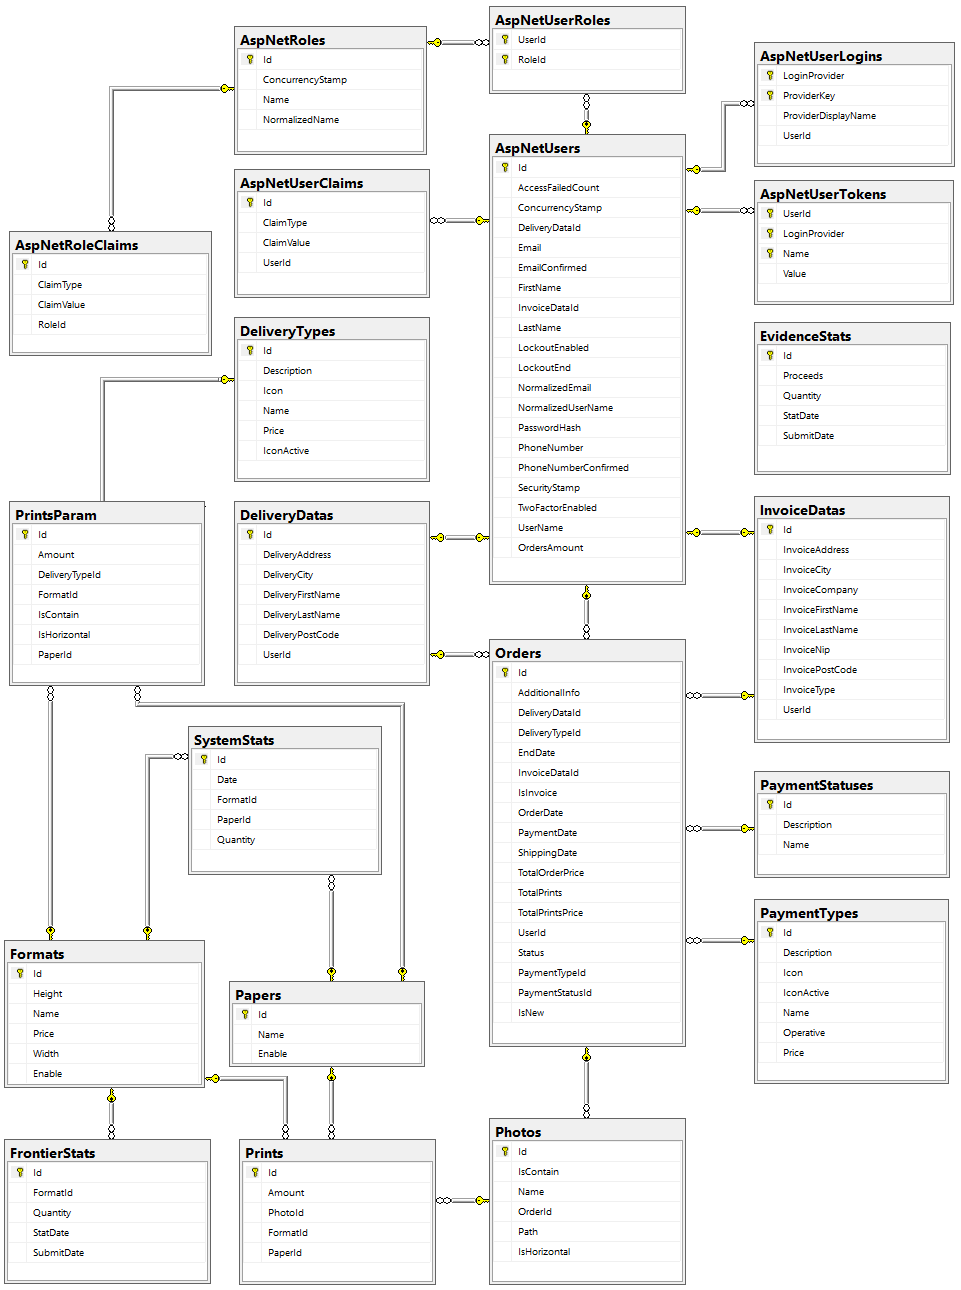
\includegraphics[width=1\linewidth]{graphics/chapter-4/database-scheme.png}
    \caption{Diagram architektury bazy danych}
    \label{fig:database-scheme}
\end{figure}



\noindent Siedem spośród przedstawionych na diagramie tabel (znajdujących się w górnej części rysunku) zawiera przedrostek \textit{AspNet}. Są to tabele wygenerowane automatycznie przez bibliotekę \textit{ASP.NET Identity} odpowiedzialną za system rejestracji i przydzielania ról użytkownikom. Tabela \textit{AspNetUsers} jako jedyna z nich posiada dodatkowe pola, które zostały dodane specjalnie na potrzeby aplikacji \textit{PhotoLab}. Wszystkie pozostałe przedstawione na diagramie tabele zostały wygenerowane poprzez przygotowanie ich odpowiednich modeli i wykorzystanie narzędzia do zmapowania ich na \textit{SQL-owe} polecenia odpowiedzialne za wygenerowanie tabel. Rdzeniem całego systemu są dwie nie tylko ,,największe'' (zawierające największą ilość atrybutów) ale i najważniejsze tabele: użytkownicy i zlecenia. Poza modułem statystyk, który funkcjonuje nieco z boku głównej funkcjonalności systemu (zamówień), wszystkie inne tabele powiązane są bezpośrednio lub pośrednio z tymi dwoma tabelami. Wartymi objaśnień wydają się powiązania z tabelą \textit{Orders}. Jak widać, każde zlecenie może mieć tylko i wyłącznie jednego właściciela (\textit{AspNetUsers}), który to z kolei może w swojej historii być twórcą wielu zleceń, a do konta mieć przypisany jeden adres dostawy. Spoglądając na powiązania z tabelą \textit{Orders} po prawej stronie diagramu widać, iż każde zlecenie zawiera takie informacje jak: rodzaj i status płatności, a~także dane do faktury i (powiązanie z lewej strony diagramu) dane do ewentualnej wysyłki (jeśli użytkownik zaznaczy takową opcję). Bardzo ważna częścią każdego zamówienia są informacje odnośnie przesłanych przez użytkownika zdjęć i parametrach ich wydruku. Informacje te zawarte są w tabeli \textit{Photos}, która występuje w relacji jeden do wielu w stosunku do tabeli \textit{Orders}. Każde zamówienie posiada listę zdjęć wgranych przez klienta do systemu. Każde zdjęcie zawiera ogólne informacje, np. o ścieżce do lokalizacji na serwerze, jego nazwie czy sposobie dopasowania w czasie wydruku, a także co najważniejsze - odwołanie do kolejnej tabeli posiadającej informacje o szczegółach dotyczących rozmiaru odbitki, papieru na którym ma zostać nadrukowana i ilości sztuk.\\
\\
Modułem niezwykle ważnym z biznesowego punktu widzenia, jednak mniej, niż moduł zleceń, związanym z całą strukturą bazy danych jest moduł statystyk laboratorium. W jego skład wchodzą trzy tabele, czyli dokładnie tyle, ile typów statystyk jest prowadzonych w ramach serwisu. Są to kolejno:
\begin{itemize}
    \item \textit{SystemStats} - generowany automatycznie, codzienny raport o wszystkich zleceniach zrealizowanych z poziomu serwisu,
    \item \textit{FrontierStats} - informacje wprowadzane ręcznie przez właściciela zakładu, comiesięczne informacje o ilości wydrukowanych zdjęć na maszynie \textit{Frontier},
    \item \textit{EvidenceStats} - również wprowadzane ręcznie, codzienne statystyki o ilości wykonanych zdjęć legitymacyjnych.
\end{itemize}


\noindent Tabele \textit{SystemStats} i \textit{FrontierStats} ściśle powiązane są z tabelami \textit{Formats} i \textit{Papers} (\textit{FrontierStats} tylko z \textit{Formats}), gdzie wyświetlają odpowiednie dane statystyczne na podstawie typów formatów i papierów. Bardzo ważnym elementem implementacji bazy danych było zapewnienie spójności danych. Należało przewidzieć zjawisko, gdzie mógłbym zostać usunięty jeden z~wcześniej dostępnych formatów lub papierów. Wówczas wszystkie powiązania związane z zamówieniem i statystykami do tych parametrów uległyby zniszczeniu, a system zawierałby ubytki w informacjach. Aby uniknąć tego zjawiska został zaimplementowany mechanizm uniemożliwiający usunięcie encji, dla których istnieje już jakiekolwiek powiązanie w systemie. Możliwym rozwiązaniem jest wówczas dezaktywacja takiego wariantu, tak aby nie był on już brany pod uwagę w dalszej pracy systemu, natomiast pozwolił zachować pełną historię wykonywanych operacji.
\newpage

\vspace*{0.01\baselineskip}

\subsection{Przetwarzanie zapytań}
\quad Głównym zadaniem serwera, którego ogólny zarys został nakreślony już we wcześniejszej części, jest przetwarzanie zapytań. W sekcji tej zostanie zaprezentowany konkretny przykład przetwarzania dwóch bardzo ważnych zadań: tworzenia zamówienia oraz wyświetlania listy wszystkich zleceń przez administratora systemu.\\
\\
\textit{Request} w postaci:

\vspace{2mm}

    \centerline{\texttt{\hl{ adres-serwera:port/api/order/submitorder }}}

\vspace{2mm}

\noindent wraz z przesyłanymi danymi oraz załączonymi w postaci nagłówków informacjami o~sposobie kodowania zapytania oraz \textit{tokenem JWT} umożliwiającym weryfikację praw dostępu użytkownika, wysyłany jest do serwera. Tam, z pomocą zaimplementowanego \textit{routing} przekierowywany jest najpierw do odpowiedniej klasy, a następnie metody - uwzględniając przy tym prawa dostępu użytkownika.\\
Tym sposobem serwer aplikacji otrzymuje od użytkownika wszystkie konieczne do założenia nowego zlecenia dane. Ponieważ użytkownik ma szeroki zakres możliwości przy konfiguracji swojego zlecenia, nie można tak otrzymanego zapytania natychmiast zapisać w bazie danych. Należy je najpierw odpowiednio przetworzyć. Dzieje się to w metodzie \textit{SubmitOrder}, klasy \textit{PhotoController}. 

\begin{listing}[ht]
    \cscode{listings/submit-order-server.cs}
    \caption{Obsługa zapytania stworzenia nowego zlecenia}
    \label{listing:submit-order-server}
\end{listing}

\noindent Parametr metody \textit{OrderVM} to otrzymane poprzez część \textit{body} zapytania HTTP dane z wypełnionego przez użytkownika formularza zlecania zamówienia. Tak otrzymane informacje w~postaci \textit{JSON} automatycznie konwertowane są na \textit{C\#-owy} \textit{ViewModel}. W przypadku powyższego zapytania ma on postać: 

\begin{listing}[ht]
    \cscode{listings/viewmodel-order-server.cs}
    \caption{\textit{ViewModel} zamówienia przesyłany do serwera aplikacji}
    \label{listing:viewmodel-order-server}
\end{listing}

\noindent Jest to zwykła klasa zawierająca listę prywatnych pól wraz z domyślnymi metodami \textit{get} i~\textit{set} do ich obsługi. Wracając do \textit{listingu \ref{listing:submit-order-server}} - tak określony model jest w linii 5 sprawdzany pod względem poprawnościowym. W przypadku niezgodności - zwracany jest błąd, a funkcja kończy działanie. Jeśli wszystko jest w porządku, przetwarzane są informacje dotyczące ewentualnej wysyłki i faktury za zamówienie. Ponieważ użytkownik ma możliwość w obu przypadkach podjęcia decyzji: czy wysyłka lub faktura jest konieczna - jeśli nie, weryfikacja ta jest pomijana, a do bazy danych zostaje zapisana bezpośrednia informacja otrzymana od klienta o braku danych na ten temat. Jeżeli użytkownik zdecyduje się na któryś z wariantów, ponownie podejmuje decyzję. Możliwe wybory to wykorzystanie danych przypisanych do jego konta lub podanie nowych informacji, przypisanych wyłącznie do tego zlecenia. Właśnie te informacje są interpretowane w liniach od 7 do 14 (ze względu na obszerność kodu, analogiczne operacje zostały pominięte). Linia numer 15 to zmapowanie, za pomocą dodatkowej biblioteki \textit{\textbf{AutoMapper}}, odpowiednio przetworzonych danych do pól modelu \textit{Order}. Kolejne linie kodu to dodanie tak utworzonego zlecenia oraz jego zależności w~postaci informacji o~zdjęciach i~konkretnych odbitkach do kontekstu (\textit{\_context}). Gdy proces ten zostanie ukończony, wystarczy zapisać zmiany w bazie danych i zwrócić odpowiedni komunikat rezultatu zapytania.\\
\\
Drugi przykład obsługi żądań przez serwer to zapytanie typu \textit{GET} - typ zapytania, które nie wysyła żadnych informacji w swojej treści, a jedynie prosi serwer o zwrócenie konkretnych danych. Omawiane zapytanie wysyłane jest pod adres:

\vspace{2mm}

    \centerline{\texttt{\hl{ adres-serwera:port/api/order/getorders }}}

\vspace{2mm}

\noindent trafiając w ten sposób do metody wskazanej w listingu poniżej.

\begin{listing}[ht]
    \cscode{listings/getorders-server.cs}
    \caption{Obsługa zapytania zwrócenia wszystkich zleceń}
    \label{listing:getorders-server}
\end{listing}

\noindent Sposób działania tej metody jest bardzo prosty. W pierwszej kolejności pobiera ona z bazy danych wszystkie znajdujące się w niej zlecenia i zapisuje w postaci listy. Poprzez dyrektywę \textit{Include} do pobranych zleceń za pomocą tzw. ładowania danych \textit{lazy loading} dołączone są informacje o użytkowniku zlecającym zamówienie. Następnie tworzona jest lista nowych, pustych \textit{ViewModeli}, które wypełniane są danymi otrzymanymi z bazy danych. Zabieg ten ma na celu ograniczenie ilości informacji,  które mają zostać przekazane aplikacji klienckiej, a zostały pobrane z bazy danych. Po pierwsze ma to wskazania wydajnościowe, po drugie bezpieczeństwa, a po trzecie ułatwia to późniejsze obsługiwanie tak uproszczonych i nie przeładowanych zawartością zapytań. Ostatnim etapem jest zwrócenie utworzonej listy i odpowiedzi z kodem typu \textit{200}.


\section{Aplikacja internetowa}
\quad Pierwsza warstwa modelu trójwarstwowego to aplikacja ukierunkowana na interakcję z użytkownikiem. Zaimplementowana jako projekt oparty o \textit{framework} \textit{Angular 4.4.6}, została podzielona na 3 podstawowe moduły, które zostaną szczegółowo nakreślone w tym rozdziale.
\newpage

\vspace*{0.01\baselineskip}

\subsection{Architektura aplikacji SPA}

        \begin{wrapfigure}[20]{l}{0.35\textwidth}
        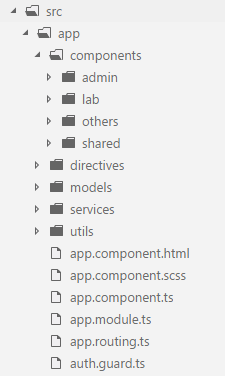
\includegraphics[width=1\linewidth]{graphics/chapter-4/client-structure.png}
        \caption{Struktura plików aplikacji klienckiej}
        \label{fig:client-structure}
        \end{wrapfigure}
            Zasadnicza struktura projektu zawarta jest w folderze \textit{src/app}. Zawiera takie elementy jak:
    \begin{itemize}

        \item Folder \textit{\textbf{components}} - zawierający komponenty czyli podstawowe składowe projektu dodatkowo podzielone na podfoldery rozdzielające poszczególne moduły aplikacji.
        \item Folder \textit{\textbf{directives}} - zbiór dodatkowych funkcjonalności, które dołączane są do \textit{drzewa DOM} dokumentu HTML w trakcie jego kompilacji.
        \item Folder \textit{\textbf{models}} - struktury odpowiedzialne za obiekty wykorzystywane w aplikacji oraz w komunikacji z serwerem.
        \item Folder \textit{\textbf{services}} - pakiet funkcji odpowiedzialnych za komunikację z serwerem i przetwarzanie rezultatów na poziomie abstrakcji danych.
        \item Pliki z serii \textit{\textbf{app}} - główne pliki \textit{Angular}, to od ich przetworzenia rozpoczyna swoje działanie cały projekt.
        \item Plik \textbf{\textit{AuthGuard}} - implementuje interfejs \textit{CanActivate}, definiując w ten sposób wymagania odpowiedzialne za dostęp do poszczególnych komponentów.
    \end{itemize}
Najważniejsza jest jednak logika podziału aplikacji na moduły i sekcje, które decydują o możliwościach jakie serwis udostępnia poszczególnym grupom użytkowników. Podział na moduły został oparty o bardzo prostą logikę poziomu dostępów oraz sposobu prezentacji witryny. Wyróżnione zostały \textbf{dwa moduły}: \textbf{administratora} oraz \textbf{laboratorium}.
\begin{figure}[ht]
	\centering
	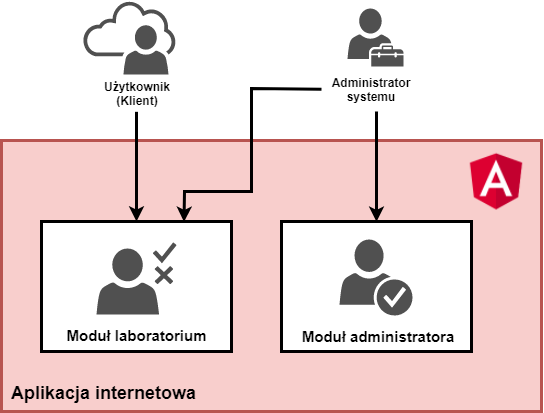
\includegraphics[width=0.75\linewidth]{graphics/chapter-4/client-architecture.png}
	\caption{Szczegółowy diagram architektury aplikacji klienckiej}
	\label{fig:client-architecture}
\end{figure}
Pierwszy z nich dostępny jest jak sama nazwa wskazuje jedynie dla osób posiadających status administratora strony. Przygotowany jest w formie panelu administracyjnego z bocznym panelem zarządzania w postaci \textit{sidebar'a}. \\Moduł laboratorium to cała dostępna dla użytkownika strona kliencka w skład której wchodzi zarówno wizytówka firmy jako strony statyczne aplikacji, jak i cały moduł zarządzania kontem użytkownika i zlecenia zamówień. Uwzględniony tam został również podział na użytkowników zalogowanych i niezalogowanych, jednak szczegółowe dotyczące dostępu do konkretnych sekcji zostaną omówione później.

\newpage
\subsubsection{Moduł Administratora}
\quad Dostęp do tej części serwisu umożliwiony jest jedynie dla zalogowanych (wyjątkiem jest strona logowania) użytkowników posiadających prawa administratora. Umożliwia on zarządzanie serwisem \textit{PhotoLab} poprzez funkcjonalności podzielone na odpowiednie podstrony tematyczne:
 \begin{itemize}
     \item \textbf{Kokpit} - składający się jedynie na podsumowanie najważniejszych informacji i statystyk dotyczących serwisu \textit{PhotoLab}.
     \item \textbf{Statystyki} - prezentacja tabelaryczna oraz w postaci wykresów wraz z możliwością dodawania i edycji danych dotyczących 3 zakresów statystyk:
        \begin{itemize}
            \item zleceń złożonych przez portal,
            \item wykonanej przez laboratorium liczby odbitek poszczególnych formatów w miesiącu,
            \item liczby wykonanych w ciągu dnia roboczego zdjęć legitymacyjnych.
        \end{itemize}
    \item \textbf{Zamówienia} - lista wszystkich zleceń z możliwością podglądu szczegółów oraz edycji niektórych parametrów zamówienia.
    \item \textbf{Użytkownicy} - podstrona prezentująca wszystkich zarejestrowanych użytkowników serwisu wraz z możliwością ich pełnej edycji.
    \item \textbf{Moje Konto} - zarządzanie ustawieniami konta obecnie zalogowanego użytkownika.
    \item \textbf{Preferencje} - sterowanie parametrami określającymi sposób działania serwisu, a także oferowanymi usługami i ich formą.
 \end{itemize}
Cały moduł oparty jest o główny komponent o nazwie \textit{layout}. Zawiera on ogólną strukturę całego szablonu panelu administracyjnego, wewnątrz którego wywoływane są inne moduły (w~oparciu o \textit{routing} aplikacji).

\begin{listing}[ht]
    \htmlcode{listings/admin-layout.html}
    \caption{Layout moduły administratora aplikacji klienckiej}
    \label{listing:admin-layout}
\end{listing}

\noindent W linii 4 i 5 importowane są statyczne komponenty nagłówka i bocznego panelu zawierającego logo oraz menu aplikacji. W linii 9 znajduje się dyrektywa odpowiedzialna za generowanie odpowiednich komponentów zgodnie ze wskazaniami \textit{trasowania}. Każdy komponent aplikacji \textit{Angular} składa się z trzech plików:
\begin{itemize}
    \item \textbf{\textit{.html}} - odpowiedzialny za generowanie struktury strony WWW,
    \item \textbf{\textit{.scss}} - plik prekompilatora \textit{Sass}, który w trakcie budowania aplikacji jest automatycznie kompilowany do kodu \textit{css} odpowiedzialnego za prezentację witryny,
    \item \textbf{\textit{.ts}} - zasadnicza część każdego komponentu - plik języka \textit{typescript} - który ostatecznie kompilowany jest do kodu języka \textit{javascript}. Jest to klasa wzbogacona o odpowiednie metadane, które pozwalają identyfikować ją jako komponent. Bazowa część komponentu to: selektor reprezentujący komponent, wskaźnik na plik szablonu i stylów oraz dodatkowe funkcje wywoływane pod wpływem zmiany stanu komponentów, jego rodzica, krewnego, potomków lub z poziomu \textit{drzewa DOM}.
\end{itemize}

\begin{figure}[ht]
	\centering
	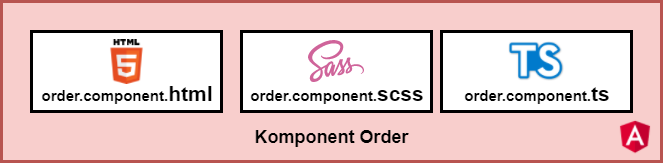
\includegraphics[width=0.75\linewidth]{graphics/chapter-4/order-component.png}
	\caption{Budowa komponentu \textit{Angular 4}}
	\label{fig:order-component}
\end{figure}
\noindent Struktury pliku \textit{.ts} jednego z najprostszych komponentów zaimplementowanych w serwisie, odpowiedzialnego za wyświetlanie listy zleceń w panelu administratora została przedstawiona na kolejnym listingu:
\newpage

\begin{listing}[ht]
    \jscode{listings/component-client.ts}
    \caption{Komponent modułu administratora serwisu \textit{PhotoLab}}
    \label{listing:component-client}
\end{listing}

\noindent W celu analizy powyższego kodu należy poruszyć kilka zagadnień:
\begin{enumerate}
    \item Linie 1-4 to import potrzebnych do obsługi komponentu danych z innych paczek, serwisów i modeli.
    \item Linie 6-10 to wspomniany wyżej dekorator zawierający alias komponentu oraz ścieżki do załączenia plików \textit{html} i \textit{css}.
    \item Od linii numer 11 zaczyna się zasadnicza część klasy komponentu. Występuje tam jego nazwa oraz informacja o implementacji dodatkowego interfejsu składającego się z jednej metody \textit{OnInit}.
    \item W konstruktorze klasy wstrzykiwana jest zależność serwisu odpowiedzialnego za obsługę zamówień (dokładne omówienie serwisów zostanie przedstawione w kolejnej sekcji).
    \item Linie 14-16 to deklaracja pól klasy wraz z inicjalizacją obiektu \textit{OrderState}.
    \item Kolejne linie to trzy funkcje: Linia 21 to implementacja interfejsu \textit{OnInit} - metoda ta wywoływana jest tylko raz, w początkowej fazie życia komponentu, tuż po wykonaniu się kodu konstruktora i pierwszego wywołania niezaimplementowanego w tym przykładzie interfejsu \textit{OnChanges}. Funkcja ta wywołuje kolejną metodę odpowiedzialną za wywołanie funkcji pobierającej dane o zamówieniu z bazy danych, znajdującej się we wstrzykniętym serwisie.
    \item Metoda \textit{getStatusName()} wywoływana jest z poziomu struktury \textit{DOM} komponentu w momencie konieczności wyświetlenia nazwy statusu zlecenia, a nie wyłącznie jego numeru.
\end{enumerate}
\subsubsection{Moduł Laboratorium}

\quad Ta część serwisu dostępna jest zarówno dla osób zalogowanych jak i anonimowych użytkowników. Podstrony objęte restrykcją dostępu są niedostępne dla użytkownika z poziomu interfejsu wystawionego przez aplikację kliencką oraz dodatkowo objęte weryfikacją posiadanych przez użytkownika uprawnień i statusu (zalogowany / niezalogowany). Przykładowo uniemożliwia to dostęp do chronionej strony poprzez wprowadzenia znanego adresu \textit{URL} do paska adresu przeglądarki internetowej. Zakres stron objętych koniecznością zalogowania użytkownika przedstawia poniższy schemat.

\begin{figure}[ht]
	\centering
	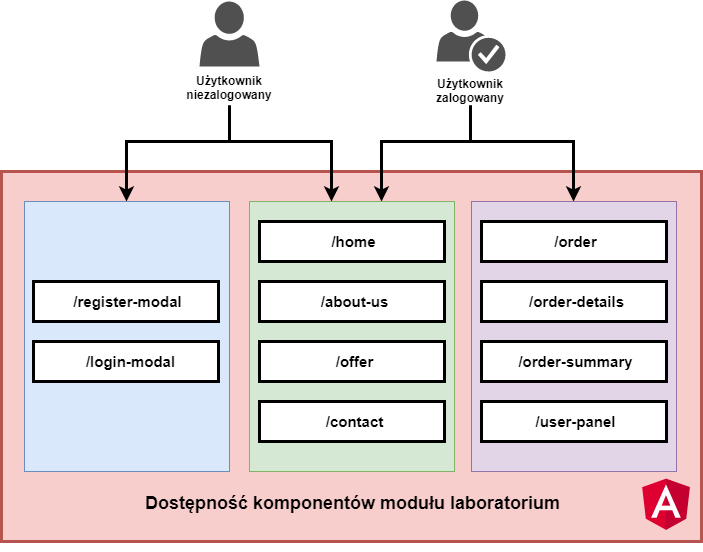
\includegraphics[width=0.8\linewidth]{graphics/chapter-4/lab-module-availability.png}
	\caption{Diagram Dostępności komponentów modułu laboratorium}
	\label{fig:lab-module-availabelity}
\end{figure}

\noindent Wszystkie strony znajdujące się na tle zielonym są to strony statyczne, tj. takie, które zawierają jedynie czysty kod \textit{html} i \textit{css}, bez dodatków w postaci dynamicznie ładowanych treści czy zachowań. Strony w niebieskim pudełku to 2 formularze służące kolejno do rejestracji nowego użytkownika oraz logowania użytkownika znajdującego się już w bazie systemu. Skonstruowane zostały w~formie tzw. \textit{okien modalnych } (\textit{modali}), czyli takich okien, które pojawiają się nad obecnie prezentowaną warstwą strony, wygaszając w ten sposób jej wszystkie funkcjonalności i powodując skupienie wzroku użytkownika (często poprzez przyciemnienie tła) na prezentowanych treściach - w tym wypadku na formularzach. \textit{Modal} znika w~momencie kliknięcia przez użytkownika jednego z proponowanych przycisków, np. \textit{anuluj} lub \textit{zapisz}/\textit{wyślij}, wykonując konkretną akcję i~powracając do widoku strony dostępnej przed pojawieniem się okna (lub przekierowując do akcji wybranej przez użytkownika).\\
\\
Również w tym module najważniejszą częścią są komponenty generujące konkretne strony lub ich fragmenty. Nie różnią się one jednak w żaden znaczący sposób od przykładowego komponentu zaprezentowanego w sekcji dotyczącej modułu administratora, dlatego też nie zostaną zaprezentowane ponownie. Pokazana natomiast zostanie budowa innych, równie ważnych elementów aplikacji \textit{Angular} - serwisów i modeli. \\
\\
Podobnie jak w aplikacji serwerowej opartej o język programowania \textit{C\#}, modele w aplikacji klienckiej służą po pierwsze do \textit{parsowania} ich do łatwo \textit{przenaszalnego} formatu~-~w~tym wypadku \textit{JSON} - by następnie mogły zostać wysłane w postaci zapytania HTTP jako dane do przetworzenia przez serwer. Drugim (nierozerwalnie powiązanym z pierwszym) zastosowaniem modeli jest przetrzymywanie informacji o danym typie danych oraz ich prezentacja i modyfikacja poprzez graficzny interfejs użytkownika w postaci strony \textit{html}. 
Przykładowa klasa modelu identycznego do tego zaprezentowanego w implementacji serwerowej została przedstawiona poniżej:

\begin{listing}[ht]
    \jscode{listings/model-client.ts}
    \caption{Model zlecenia w aplikacji klienckiej}
    \label{listing:model-client}
\end{listing}

\noindent Jedyną różnicą w prezentowanej strukturze (w porównaniu z implementacją serwerową) jest fakt zastosowania składni innego języka programowania (\textit{Typescript} vs. \textit{C\#}). Różnicą, jaką można zauważyć to definiowanie wszystkich pól automatycznie jako publiczne oraz umiejscowienie ich jako parametry konstruktora klasy. Jest to celowy zabieg umożliwiający w \textit{Typescript}  definiowanie elementów klasy automatycznie z określaniem ich parametrów dla domyślnego konstruktora bezparametrowego. W ten sposób można wyzbyć się nadmiernego tworzenia prawie identycznego kodu.\\
\\
\noindent W klienckiej aplikacji \textit{Photolab} serwisy pełnią cztery zasadnicze role:
\begin{itemize}
    \item jako jedyne struktury zawierają funkcje odpowiedzialne za komunikację z serwerem,
    \item zawierają metody, które są wykorzystywane przez co najmniej dwa komponenty jednak zazwyczaj są to metody, które wywoływane są w większości komponentów w tej samej formie. Ich implementacja w poszczególnych komponentach byłaby niepotrzebną redundancją kodu,
    \item przechowują obiekty, których okres występowania nie ogranicza się jedynie do jednego komponentu (np. obiekt \textit{order} - występuje w całym procesie zlecania zamówienia, tj. w~komponentach: \textit{order}, \textit{orderDetails} i \textit{orderSummary}),
    \item służą jako pośrednik w wymianie informacji pomiędzy komponentami, np. poprzez rozgłaszanie informacji do nasłuchujących komponentów.
\end{itemize}

\noindent Wszystkie powyżej wymienione funkcjonalności serwisów zostały zaprezentowane w~listingu \ref{listing:service-client} przedstawiającym fragmenty serwisu \textit{Order} służącego do obsługi procesu zlecania zamówienia w module laboratorium.

\begin{listing}[ht]
    \jscode{listings/service-client.ts}
    \caption{Serwis obsługi zlecania zamówień w module laboratorium}
    \label{listing:service-client}
\end{listing}

\noindent Linie 3-8 to pola dostępne do użytku wewnętrznego przez serwis lub do udostępnienia jednolitych danych wielu komponentom (np. pole \textit{order}). Metoda \textit{getFormatPrice(...)} to doskonały przykład bardzo prostej funkcji wykorzystywanej przez wiele komponentów w celu zwrócenia ceny formatu odbitki posiadając jedynie wiedzę o jej numerze identyfikacyjnym. Kolejna funkcja \textit{setOrderStatus(...)} jest egzemplarzem rodziny funkcji wysyłającej do serwera zapytanie \textit{HTTP}. W tym przypadku jest to zapytanie typu \textit{GET} proszące o zwrócenie liczby (oczekiwanie wartości typu \textit{Observable<number>}) zleceń ze statusem ,,nowe''. Gdy taka odpowiedź nadejdzie, należy ją zwrócić w postaci rezultatu wykonania funkcji lub w przypadku błędu przekierować go do funkcji wstrzykniętego do klasy serwisu \textit{ConfigService} odpowiedzialnego za obsługę błędów zapytań po stronie aplikacji. Ostatnia z głównych funkcjonalności serwisów została zaprezentowana na przykładzie w linii 24. Jest to funkcja odpowiedzialna za propagowanie wiadomości o zaistniałym zdarzeniu do innego, nasłuchującego na ten typ wiadomości kontrolera.
\newpage
\subsection{Warstwa prezentacji}
\quad Tworząc aplikację dostępną dla szerokiego grona użytkowników bardzo ważne jest zadbanie o~spójny, estetyczny wygląd oraz łatwą i intuicyjną strukturę serwisu, a także wyeksponowanie najważniejszych z biznesowego punktu widzenia elementów strony.\\
\\
Aby osiągnąć takowy efekt konieczne jest zbudowanie poprawnej oraz logicznej struktury \textit{drzewa DOM}, a także zapewnienie odpowiedniej formy prezentacji tych danych przy wykorzystaniu \textit{kaskadowych arkuszy stylów} (\textit{css}). W celu ułatwienia i stanowczego przyspieszenia prac w~projekcie został zaimplementowany \textit{framework CSS} - \textit{\textbf{Bootstrap}} w obecnie najnowszej wersji \textit{4.0.0} (będącej jeszcze wersją beta).\\
\\
Najważniejszymi elementami wykorzystanymi z tej biblioteki były przede wszystkim klasy opisujące strukturę dokumentu, tj. \textbf{\textit{FlexBox}} i \textbf{\textit{Bootstrap Grid}}. Ich implementacja była stosowana zamiennie lub w sposób mieszany w zależności od złożoności i konkretnych wymagań danej sekcji.\\
\\
Zamiast zwykłej składni \textit{CSS} (\textit{.css}) została użyta składnia preprocesora \textit{SASS} (\textit{.scss}) umożliwiającego bardziej zaawansowane operowanie na kaskadowych arkuszach stylów poprzez różnego rodzaju \textit{mixiny}, \textit{zmienne}, \textit{zagnieżdżenia}, itp. Przykład kilku wybranych fragmentów kodu implementujących najwięcej funkcjonalności udostępnianych przez preprocesor języka \textit{CSS} został przedstawiony poniżej:

\begin{listing}[ht]
    \sasscode{listings/sass-example.scss}
    \caption{Demonstracja możliwości preprocesora \textit{Sass}}
    \label{listing:sass-example}
\end{listing}

\noindent Powyższy kod wydaje się być na tyle prosty i intuicyjny, iż nie wymaga większych objaśnień. \textit{@mixin} to zestawy reguł zebranych pod jednym \textit{aliasem}, które bez zbędnych powtórzeń można wykonywać wielokrotnie w kodzie. Znakiem \textit{\$} rozpoczyna się nazwa zmiennej, do której np. można przypisać odpowiednią wartość koloru. Następnie w momencie potrzeby zmiany odcieniu wszystkich elementów \textit{ostylowanych} danym rodzajem koloru, nie jest konieczne dokonywanie zmian w wielu miejscach, wystarczy jedna zmiana, w definicji zmiennej. \\
\\
Aplikacja \textit{PhotoLab} to jednak nie tylko efekty generowane przez arkusze stylów. To również liczne grafiki, ikony i obrazy. Wszystkie wymienione (z wyjątkiem kilku elementów, które są własnością autora pracy) zostały zaczerpnięte z licznych stron internetowych. W~trakcie ich selekcji zostały uwzględnione ustanowione dla nich prawa autorskie. Większość wykorzystanych fotografii pochodzi z serwisu \textit{Pexels.com}, który udostępnia wysokiej jakości fotografie w~większości na licencji \textit{CC0} - oznaczającej ,,Brak zastrzeżonych praw autorskich'' (\textit{ang. no copyright reserved}). Natomiast jeżeli chodzi o wykorzystane ikony, to ich jedynym źródłem jest portal \textit{FontAwesome.io} oferujący dodatkową bibliotekę udostępniającą szeroki zakres ikon w postaci wektorów, które można dostosowywać do własnych potrzeb poprzez zmianę np. koloru czy rozmiaru. Ikony te udostępnianie są na licencji \textit{SIL Open Font License}, oznaczającą pełną dowolność w ich wykorzystaniu.
\newpage

\vspace*{0.01\baselineskip}

\section{Środowisko produkcyjne}
\quad Aplikacja w trakcie procesu jej powstawania była budowana, uruchamiana i testowana w oparciu o \textit{\textbf{środowisko deweloperskie}}. Różni się ono od \textit{\textbf{środowiska produkcyjnego}} w kilku aspektach. Ogólnie mówiąc otoczenie programistyczne zawiera więcej dodatkowych informacji mających na celu możliwość \textit{debugowania} i sprawdzenia tworzonego kodu. Pliki nie są w pełni skompresowane, a np. ścieżki odnoszą się często do innych, również tymczasowych (na czas implementacji) lokalizacji. Dodatkowo należy zaznaczyć, iż cały proces budowania i uruchamiania aplikacji odbywa się (w przypadku \textit{PhotoLab}) lokalnie na komputerze programisty. Tak wygenerowany projekt nie może być po prostu przeniesiony 1:1 na zewnętrzny hosting. Należy go odpowiednio przygotować i osadzić na odpowiednim do tego serwerze, a następnie uruchomić. Konieczne do zakończenia tego procesu sukcesem kroki zostały przedstawione w tej części rozdziału. Na koniec została umieszczona również skrócona instrukcja użytkowania aplikacji prezentująca jego najważniejsze elementy i funkcjonalności.

\subsection{Proces instalacji}
\quad W tej sekcji zostanie zaprezentowana ogólna instrukcja postępowania mającego na celu wygenerowanie projektu w wersji produkcyjnej oraz jego późniejsze wdrożenie (\textit{ang. deploy}) na zewnętrznym serwerze pełniącym rolę hostingu aplikacji.\\
\\
Zaprezentowany sposób nie jest z pewnością najbardziej optymalny i służący do masowego i ciągłego aktualizowania wersji produkcyjnej oprogramowania. Rozwiązanie takie można zautomatyzować, np. w taki sposób aby wszelkie zmiany naniesione w projekcie i~zapisane na zdalnym repozytorium były automatycznie wdrażane na serwer produkcyjny. Na potrzeby aplikacji \textit{PhotoLab} proces przygotowywania takiego środowiska wdrożeniowego został jednak maksymalnie uproszczony i wymaga ręcznego aktualizowania (ponownego \textit{deploymentu}) wszelkich zmian. Jak prezentuje się zaproponowane i wdrożone środowisko produkcyjne dla aplikacji \textit{PhotoLab} zostało to przedstawione na rysunku \ref{fig:production-server}).

\begin{figure}[ht]
	\centering
	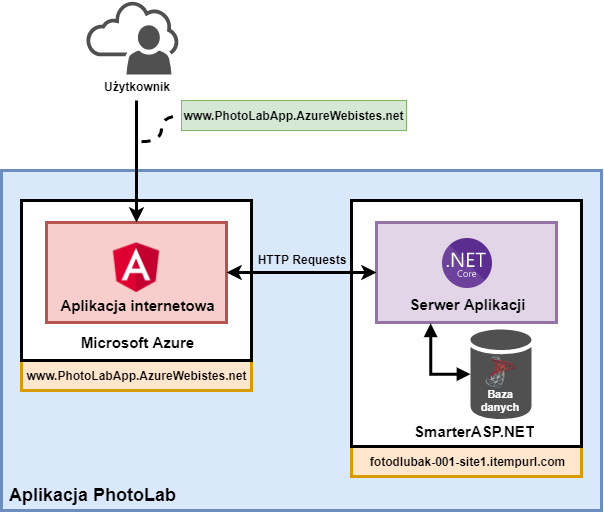
\includegraphics[width=0.8\linewidth]{graphics/chapter-4/production-server.png}
	\caption{Środowisko produkcyjne aplikacji}
	\label{fig:production-server}
\end{figure}

\subsubsection{Wdrożenie aplikacji klienckiej}
\quad Aplikacja kliencka została opublikowana na serwerze znajdującym się w usługach chmurowych oferowanych przez firmę \textit{Microsoft} - \textbf{\textit{Azure}}. Powodem wyboru tego konkretnego usługodawcy jest przede wszystkim zerowy koszt utrzymania. \textit{Azure} w darmowym planie oferowanym przez studencki program partnerski \textit{DreamSpark} w zupełności wystarcza swoimi parametrami technicznymi spełnić wymagania aplikacji \textit{Angular}. Dodatkowo jest on bardzo szybki i zapewnia jedną z najwyższych na rynku dostępności serwera (bardzo dobra stabilność).\\
\\
Proces \textit{deploymentu} należy rozpocząć od zbudowania aplikacji w sposób przeznaczony do działania na serwerze produkcyjnym. W czasie implementacji proces budowania polegał na wykonywaniu komendy:

\vspace{2mm}

    \centerline{\texttt{\hl{ npm start }}}

\vspace{2mm}

\noindent W przypadku potrzeby wygenerowania projektu produkcyjnego należy użyć komendy:

\vspace{2mm}

    \centerline{\texttt{\hl{ ng build --prod }}}

\vspace{2mm}
\noindent W pierwszej jednak kolejności należy założyć konto hostingowe dla serwera (opis w kolejnej sekcji) i w pliku \textit{config.service.ts} podmienić adres \textit{apiURI} na adres WWW serwera wraz z dopisanym na końcu ścieżki - \textit{/api}. Po tym kroku można wykonać powyższą komendę.
Projekt zostanie odpowiednio utworzony w wyznaczonym przez plik \textit{angular-cli.json} miejscu. Dla \textit{PhotoLab} jest to:

\vspace{2mm}

    \centerline{\texttt{\hl{ /Server/wwwroot/ }}}

\vspace{2mm}

\noindent Kolejnym krokiem jest dodaniem do korzenia tak utworzonego projektu (po zbudowaniu projektu, korzeniem staje się folder \textit{/Server/wwwroot}) pliku \textit{web.config} odpowiedzialnego za konfigurację serwera \textit{IIS} odpowiedzialnego za uruchomienie i odpowiednie mapowanie aplikacji na hostingu \textit{Azure}. Kod źródłowy  pliku został zaczerpnięty ze źródła \cite{deploying-angular}.
\newpage

\begin{listing}[ht]
    \xmlcode{listings/web-config.xml}
    \caption{Zawartość pliku \textit{web.config} koniecznego do wdrożenia aplikacji klienckiej}
    \label{listing:web-config}
\end{listing}

        \begin{wrapfigure}[18]{l}{0.4\textwidth}
        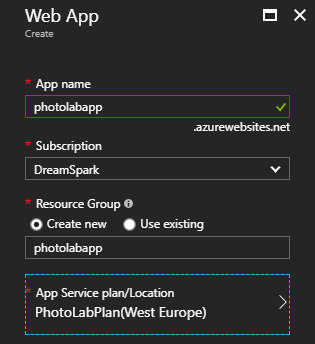
\includegraphics[width=1\linewidth]{graphics/chapter-4/azure-deploy.png}
        \caption{Tworzenie nowej aplikacji Azure}
        \label{fig:azure-deploy}
        \end{wrapfigure}
\noindent Gdy plik zostanie dodany, należy przejść do drugiego etapu wdrożenia. Założenia nowej aplikacji w~portalu \textit{Azure}. W tym celu należy zalogować się na swoje konto do portalu \texttt{https://portal.azure.com}, następnie przejść do zakładki \textit{App Services}, kliknąć przycisk \textit{Add} i~wybrać aplikację typu \textit{Web App}. Kolejnym krokiem jest podanie wymaganych parametrów (Rys. \ref{fig:azure-deploy}). Aplikacja zostanie utworzona. W~zakładce \textit{Deployment credentials} należy ustawić dane dostępowe do serwera \textit{FTP} zgodnie z~własnymi preferencjami.       
 Gdy takowe zostaną określone, wystarczy wykorzystać je do zalogowania się do serwera \textit{FTP} za pomocą dowolnego klienta \textit{FTP} (np. \textit{Total Commander} i przekopiowanie plików z folder \texttt{wwwroot} do katalogu \texttt{site/wwwroot}. \\
 \\
 Aplikacja została poprawnie wdrożona na serwer - adres serwera \textit{FTP} jak i adres \textit{URL} strony na której hostowana jest aplikacja znajduje się w prawej górnej części zakładki \textit{Overview}.
\newpage

\vspace*{0.01\baselineskip}

\subsubsection{Wdrożenie serwera aplikacji i bazy danych}
\quad Aplikacja biznesowa wraz z bazą danych zostały zainstalowane na serwerze obsługiwanym przez firmę \textit{SmarterASP.NET}. Darmowy, 60 dniowy okres testowy wystarczył, aby stwierdzić, iż serwis ten umożliwia stosunkowo proste wdrożenie aplikacji wraz z dołączoną do niej bazą danych. Dodatkowo pierwszy dostępny pakiet cenowy przedstawia bardzo dobry stosunek oferowanych możliwości do kosztów, gdzie zarówno pierwszy, jak i drugi - spełniają wymagania dotyczące serwera produkcyjnego dla aplikacji \textit{PhotoLab}.
        \begin{wrapfigure}[19]{l}{0.35\textwidth}
        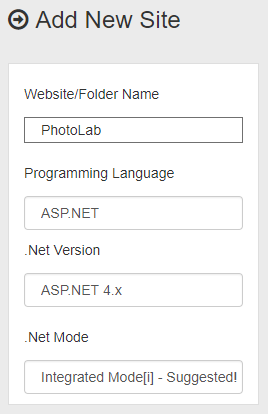
\includegraphics[width=1\linewidth]{graphics/chapter-4/server-account.png}
        \caption{Tworzenie aplikacji smarterASP.NET}
        \label{fig:server-application}
        \end{wrapfigure}
        
\noindent Wdrożenie należy rozpocząć od rejestracji nowego konta w serwisie \textit{SmarterASP.NET}. Następnie należy przejść do panelu zarządzania i z zakładki \textit{Hostings} wybrać przycisk \textit{+~Add New Hosting Account} by utworzyć nowe konto hostingowe. Gdy jest ono gotowe należy z panelu zarządzania hostingiem wybrać \textit{Websites} i zielony przycisk \textit{New Site} w~celu utworzenia struktury nowej aplikacji. Parametry inicjalizacyjne należy ustawić tak jak przedstawiono to na rys. \ref{fig:server-application}.
 Aplikacja zostanie utworzona. Należy pobrać dane wdrożeniowe (\textit{ang. WebDeploy Info}) rozwijając pole \textit{Show WebDeployInfo} i~klikając przycisk \textit{Get Publish Setting} - rysunek \ref{fig:webdeploy-info}.
 
 Kolejnym etapem jest przejście do zakładki \textit{Databases} i~utworzenie bazy danych typu \textit{MSSQL Database}. Gdy baza zostanie stworzona należy postępować podobnie jak w przypadku pobierania \textit{WebDeploy Info}. Rozwinąć zakładkę \textit{Connection String Examples} i zapisać \textit{Connection String} przeznaczony dla aplikacji \textit{ASP.NET}.
 
 \vspace{15mm}
 
\begin{figure}[ht]
	\centering
	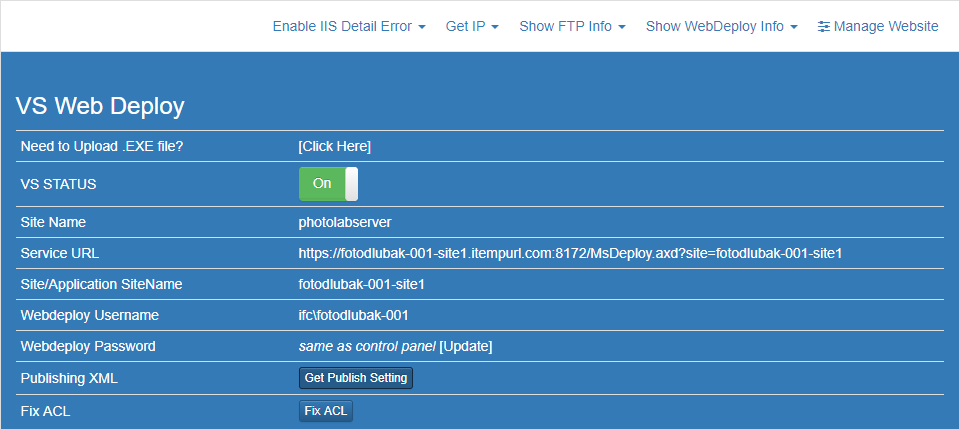
\includegraphics[width=1\linewidth]{graphics/chapter-4/server-webdeploy-info.png}
	\caption{Profil danych koniecznych do wdrożenia serwera}
	\label{fig:webdeploy-info}
\end{figure}

\noindent Ostatnie prace wymagają otwarcia projektu serwera aplikacji w~środowisku \textit{Visual Studio}. Tam w pliku \textit{AppSettings.json} należy podmienić lokalny \textit{Connection String} na ten skopiowany z~utworzonej bazy danych i na jego końcu wprowadzić ustalone do bazy danych hasło. Następnie należy kliknąć \textit{PPM} na nazwę projektu w oknie solucji (\textit{ang. Solution Explorer}) i wybrać publikuj (\textit{ang. publish}).\\
\\
\noindent Kolejne kroki, które należy wykonać to:
 \begin{enumerate}
     \item \textit{Create new profile} -> \textit{import profile} -> \textit{ok}.
     \item Z okna systemowego - wybór pobranego wcześniej profilu.
     \item Z prawej strony rubryki \textit{Summary} wybór: \textit{Settings}.
     \item Wprowadzenie hasła do aplikacji i zweryfikowanie połączenia - \textit{Validate Connection}.
     \item W zakładce \textit{Settings}, ustawienie parametrów jak na rys \ref{fig:server-visual-deploy}, gdzie w polu \textit{ConnectionString} podany jest wcześniej skopiowany link ze zmienionym na końcu hasłem.
     \item Wybranie \textit{Save}, a następnie \textit{Publish}.
 \end{enumerate}
 
 
   \begin{figure}[ht]
	\centering
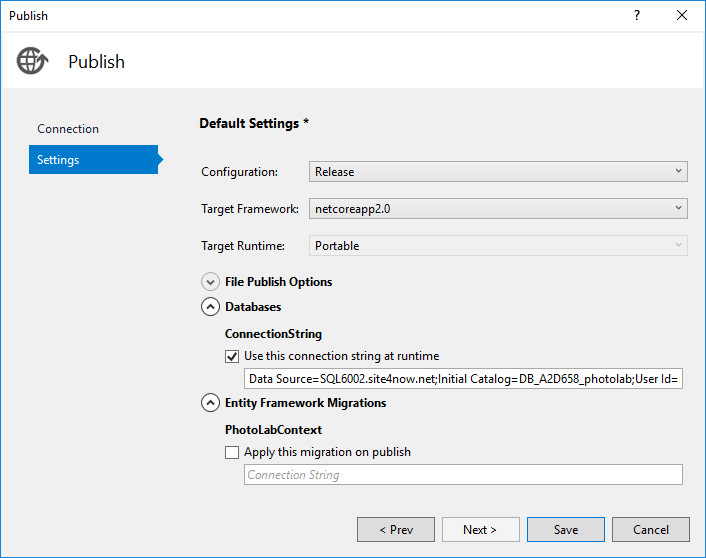
\includegraphics[width=0.7\linewidth]{graphics/chapter-4/server-visual-deploy.png}
\caption{Ustawienia profilu wdrożenia w Visual Studio}
\label{fig:server-visual-deploy}
\end{figure}     
\noindent Po chwili oczekiwania, aplikacja zostanie poprawnie zainstalowana.
Ostatnim wymaganym krokiem jest wykonanie kopii bazy danych (np. poprzez aplikację \textit{Microsoft SQL Server Management Studio}, a następnie jej wgranie na serwer w menu \textit{Databases}, wybierając \textit{Actions}, \textit{Restore Database} i zaznaczając plik kopii bazy danych. Na tym etapie proces wdrożenia dobiegnie końca - strona dostępna jest pod adresem \textit{http://photolabapp.azurewebsites.net}.
\newpage

\vspace*{0.01\baselineskip}

\subsection{Przewodnik użytkownika}
\quad Z racji rozbudowanego interfejsu użytkownika, który zawiera około 30 różnych widoków aplikacji, instrukcja zostanie oparta jedynie o najważniejsze elementy całego serwisu, które są przedstawicielami kategorii poszczególnych stron. Uwzględniony został również podział prezentowanych treści na dwa moduły, które zasadniczo się od siebie różnią - wyglądem, dostępem dla użytkowników i funkcjonalnościami.

\begin{figure}[ht]
	\centering
	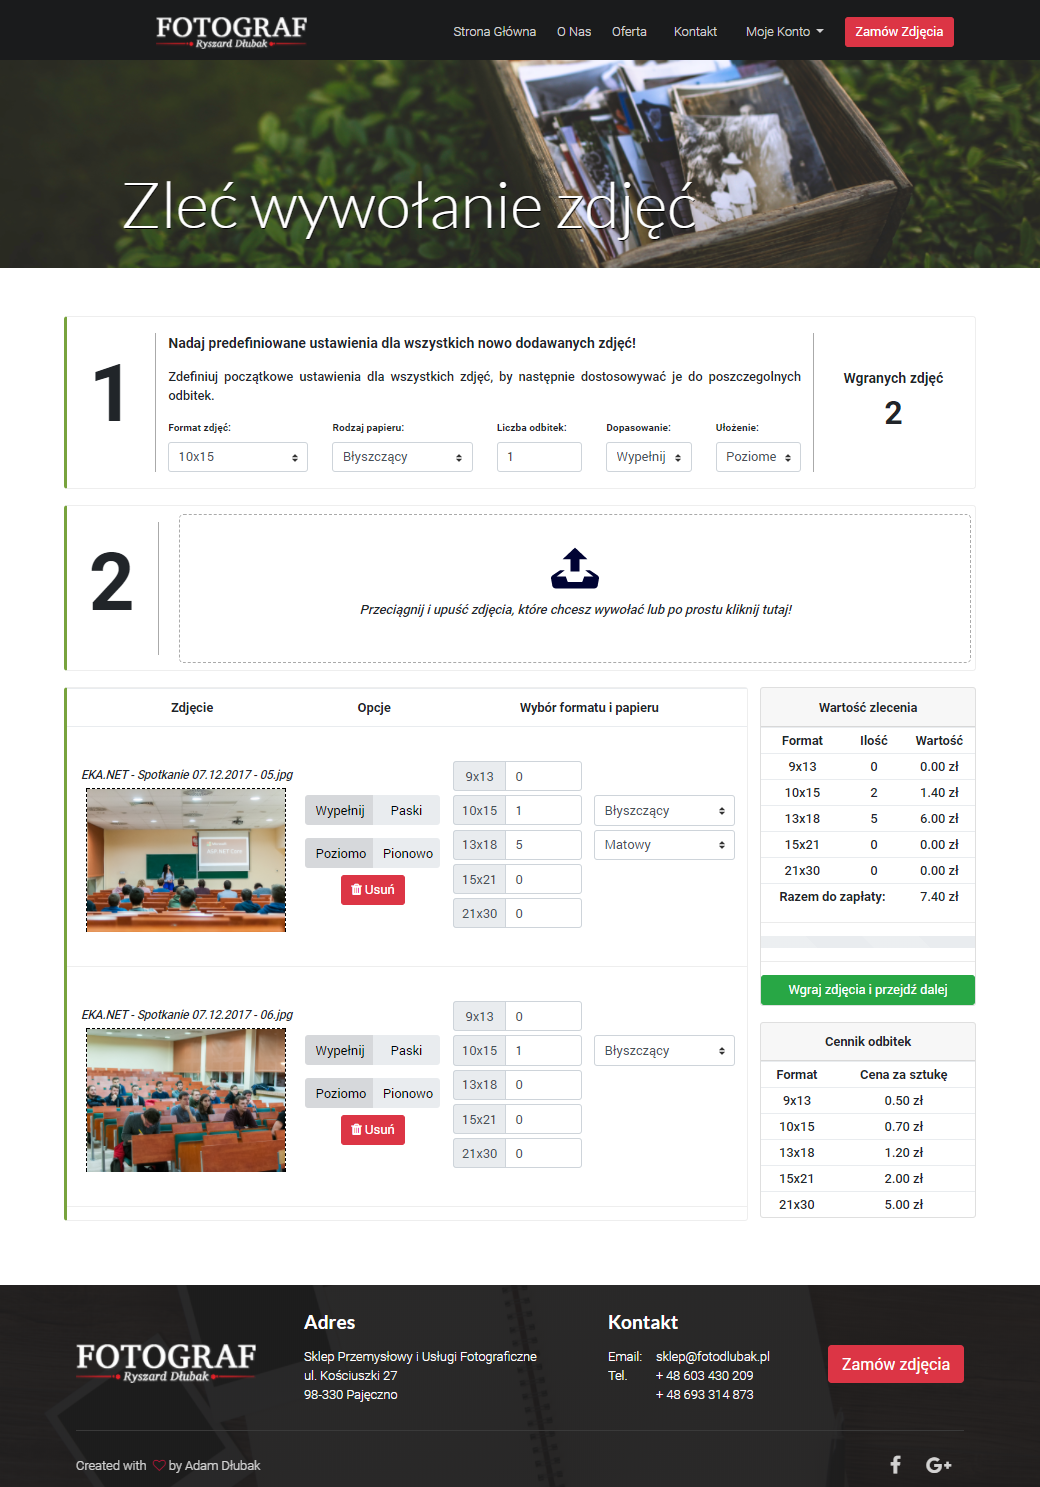
\includegraphics[width=0.85\linewidth]{graphics/chapter-4/screen-1.png}
	\caption{Ogólny widok modułu laboratorium wraz z funkcją zamawiania odbitek}
	\label{fig:screen-1}
\end{figure}
\newpage

\vspace*{0.01\baselineskip}



\subsubsection{Moduł Laboratorium}
\quad Najważniejszym widokiem tego modułu jest oczywiście część odpowiedzialna za \textbf{zlecanie zamówienia} na wykonanie usługi. Pierwszy etap tego procesu wraz z całym kontekstem strony (nagłówek, stopka) został przedstawiony na rysunku \ref{fig:screen-1}. Doskonale widać tam 4 etapy wyboru i parametryzacji zdjęć:
\begin{itemize}
    \item etap 1 - wybór domyślnych parametrów dla wszystkich nowo dodawanych zdjęć,
    \item etap 2 - wgrywanie zdjęć; dwie możliwości - wybór z okna systemowego po kliknięciu w~dostępne pole lub wykorzystanie funkcjonalności ,,przeciągnij i upuść'',
    \item etap 3 - dokładne ustalenie ilości i rodzaju odbitek dla poszczególnych fotografii,
    \item etap 4 - podsumowanie zlecenia i przesłanie plików oraz przejście do kolejnego etapu zamówienia - danych wysyłki, potwierdzenia zakupy i sposobu płatności.
\end{itemize}

\noindent Innym bardzo ważnym zadaniem systemu jest identyfikacja klientów laboratorium. Aby mieć możliwość zlecenia zamówienia, użytkownik zobligowany jest do założenia konta w serwisie, a~następnie za jego pomocą zalogowania się do systemu. \\
\\
Widok \textbf{logowania użytkownika} został przedstawiony na kolejnym rysunku (rys. \ref{fig:screen-2}). Zarówno logowanie jak i rejestracja zostały zaimplementowane w postaci pojawiających się okien - \textit{modali}. Umożliwia to sprawne i wygodne dokonanie autentykacji użytkownika bez opuszczania kontekstu strony, w której się znajdował.

\begin{figure}[ht]
	\centering
	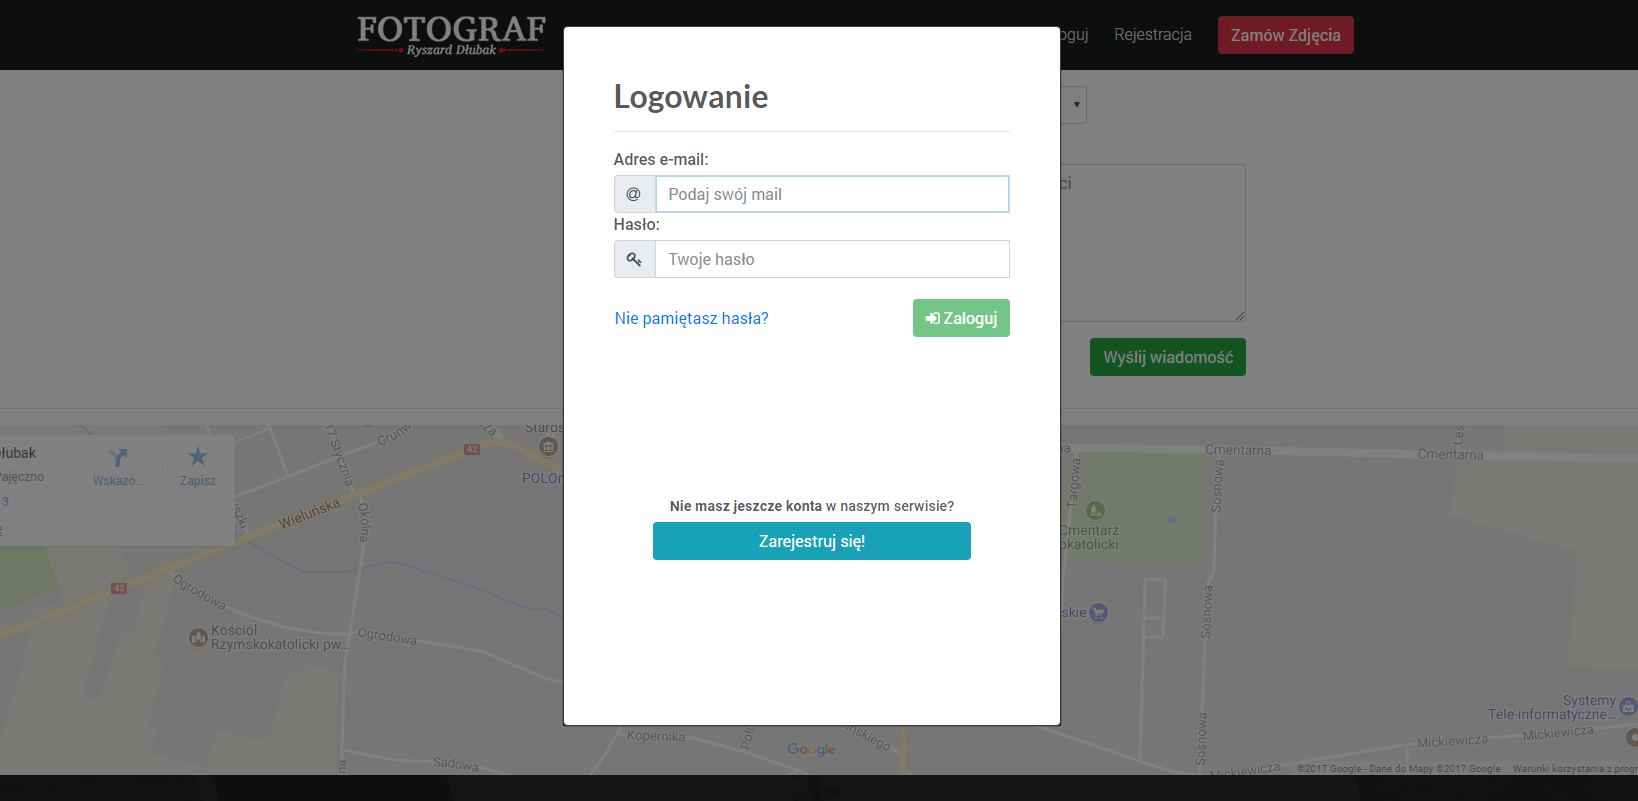
\includegraphics[width=0.9\linewidth]{graphics/chapter-4/screen-2.png}
	\caption{Widok logowania użytkownika}
	\label{fig:screen-2}
\end{figure}

\noindent Klient po zalogowaniu, korzystając z odpowiedniego odnośnika znajdującego się w nagłówku strony (\textit{ang. header}) może przejść do \textbf{panelu użytkownika}. Tam ma możliwość dostosowywania takich parametrów swojego konta jak: podstawowe dane (imię, nazwisko, numer telefonu, adres e-mail), dane do wysyłki zamówienia, dane do faktury, czy zmiana obecnego hasła do konta. Ponadto ma on możliwość przeglądania swoich, zarówno obecnych, jak i już zrealizowanych zleceń.

\begin{figure}[ht]
	\centering
	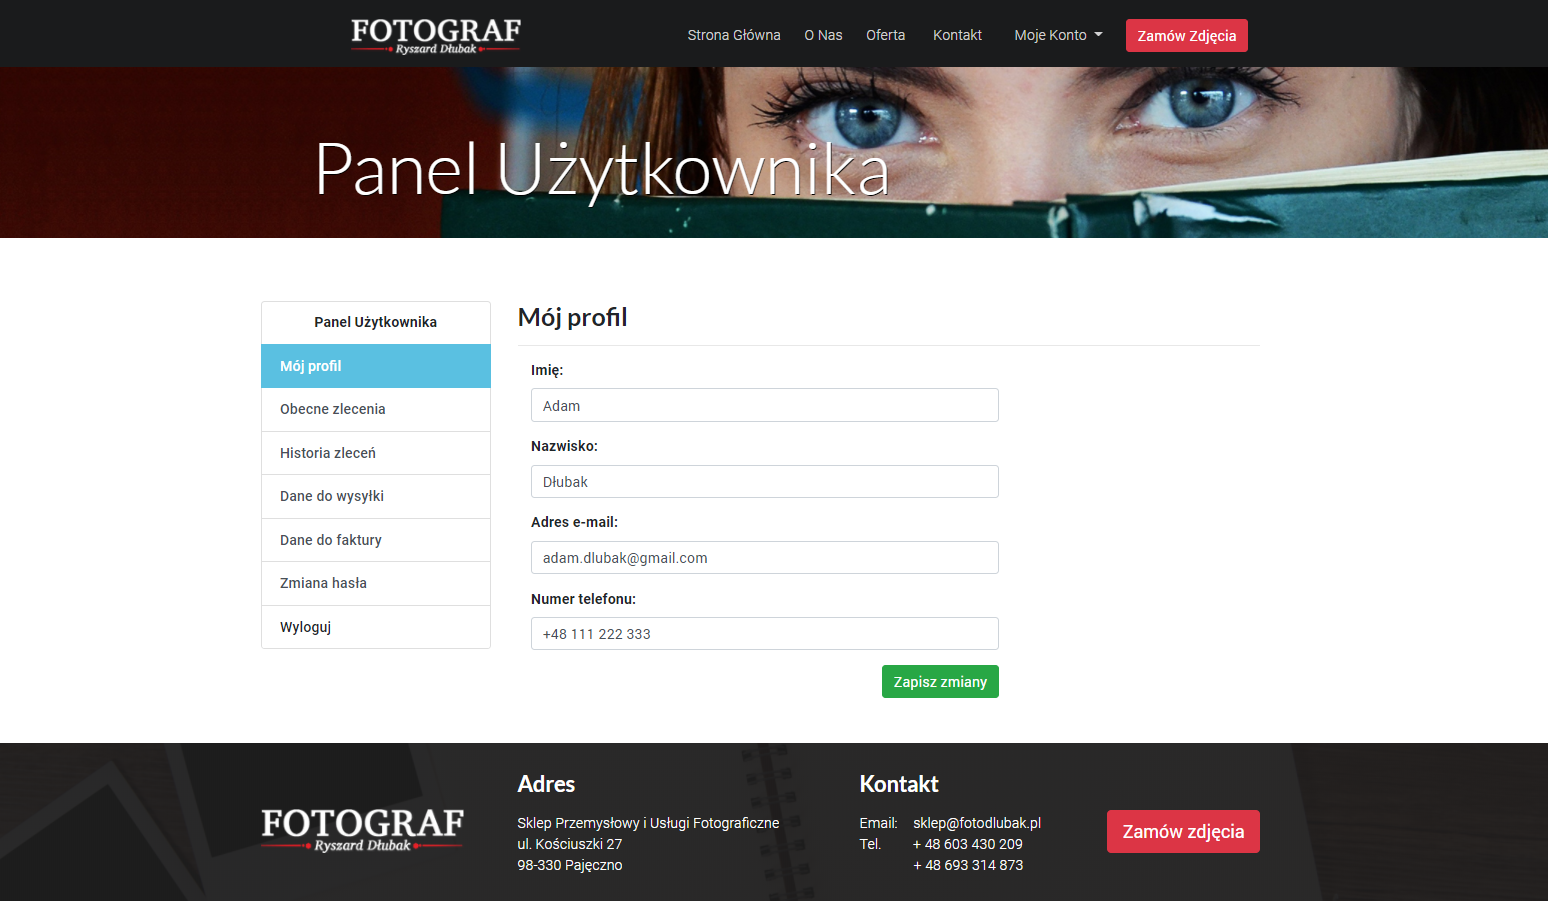
\includegraphics[width=0.85\linewidth]{graphics/chapter-4/screen-3.png}
	\caption{Widok panelu użytkownika}
	\label{fig:screen-3}
\end{figure}

\noindent Oczywiście serwis dostępny dla klienta to nie tylko widoki odpowiedzialne za generowanie zamówień, czy obsługę konta. To również strony prezentujące informacje o firmie, tzw. wizytówki. Wszystkie z tych stron zostały stworzone jako \textbf{strony statyczne}, tj. takie, które nie zawierają treści dynamicznych (np. pobieranych z bazy danych). Jedną z takich stron jest z pewnością podstrona \textit{Kontakt} prezentująca podstawowe informacje o firmie, jej adres, pełną nazwę i dane kontaktowe, a także mapę z zaznaczoną lokalizacją. Ponadto udostępnia ona formularz pozwalający bezpośrednio z poziomu strony internetowej wysłać wiadomość e-mail do laboratorium.

\begin{figure}[ht]
	\centering
	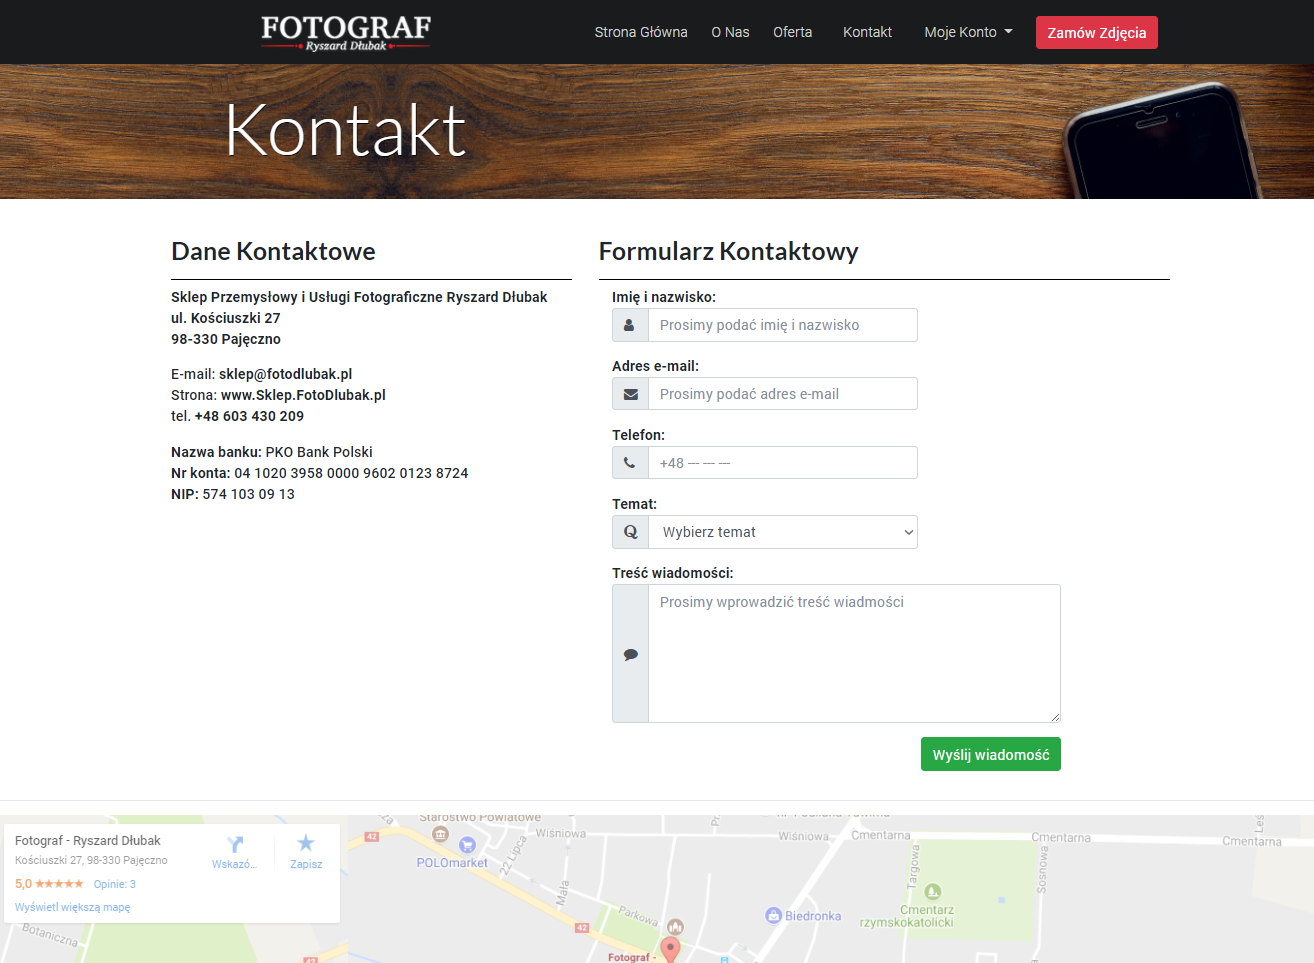
\includegraphics[width=0.85\linewidth]{graphics/chapter-4/screen-4.png}
	\caption{Widok statycznej strony kontaktu}
	\label{fig:screen-4}
\end{figure}

\newpage




\newpage

\vspace*{0.01\baselineskip}


\subsubsection{Moduł Administratora}
\quad Ta część serwisu dostępna jest jedynie dla użytkowników posiadających przedzieloną rolę administratora. Ze względu na swój charakter i prezentowane treści jej \textit{layout} różni się od tego, który udostępniany jest pozostałym użytkownikom aplikacji. Jego zasadnicza część znajduję się po lewej stronie w postaci \textit{sidebara}. Można tam wyróżnić dwa elementy: logo serwisu oraz menu, które umożliwia nawigację do poszczególnych funkcjonalności panelu.\\
\\
Rdzeniem całego modułu jest sekcja dotycząca zamówień. Poprzez wybranie przycisku \textit{Zamówienia}, administratorowi udostępniana jest lista wszystkich zamówień znajdujących się w~systemie. Lista udostępnia takie informacje o zamówieniu jak: data zlecenia, zleceniodawca, ilość odbitek i wartość całego zamówienia, a także jego status. Dodatkowo możliwa jest nawigacja do szczegółów danego zamówienia. Widok ten został zaprezentowany na rysunku \ref{fig:screen-5}.


\begin{figure}[ht]
	\centering
	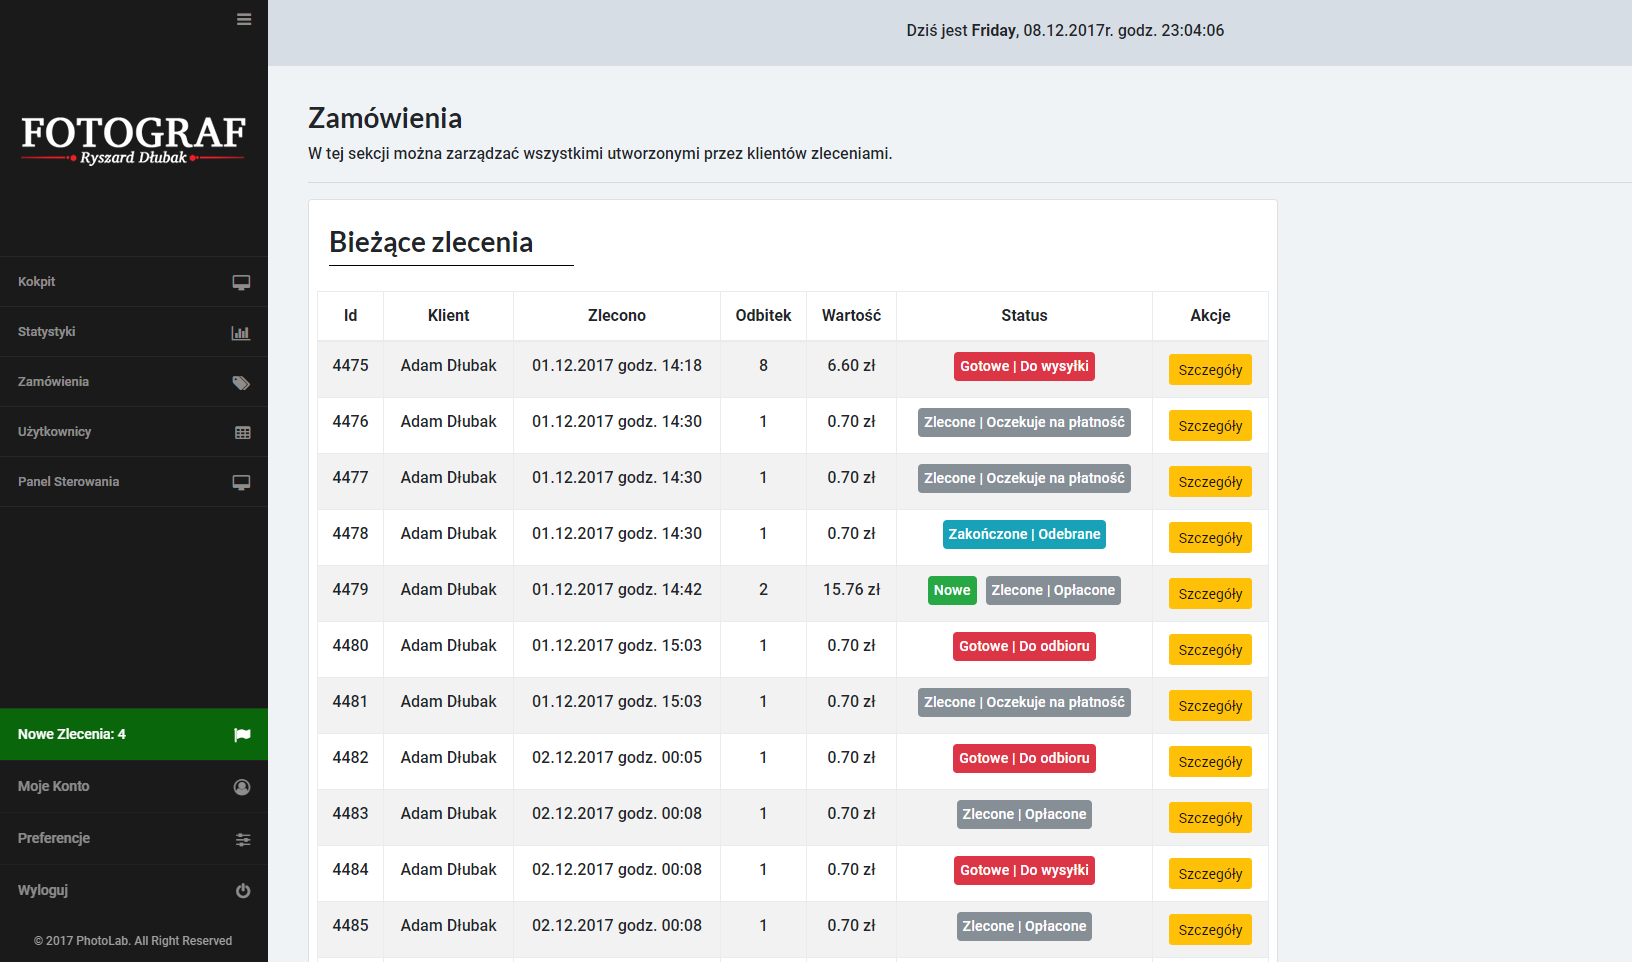
\includegraphics[width=0.9\linewidth]{graphics/chapter-4/screen-5.png}
	\caption{Widok listy zleceń w panelu administratora}
	\label{fig:screen-5}
\end{figure}

\noindent Aby zrealizować zlecenie według wskazań klienta, pracownik zakładu powinien skorzystać z~podglądu całej konfiguracji zlecenia. Udostępnia to kolejny widok zaprezentowany na rysunku \ref{fig:screen-6}.


\begin{figure}[ht]
	\centering
	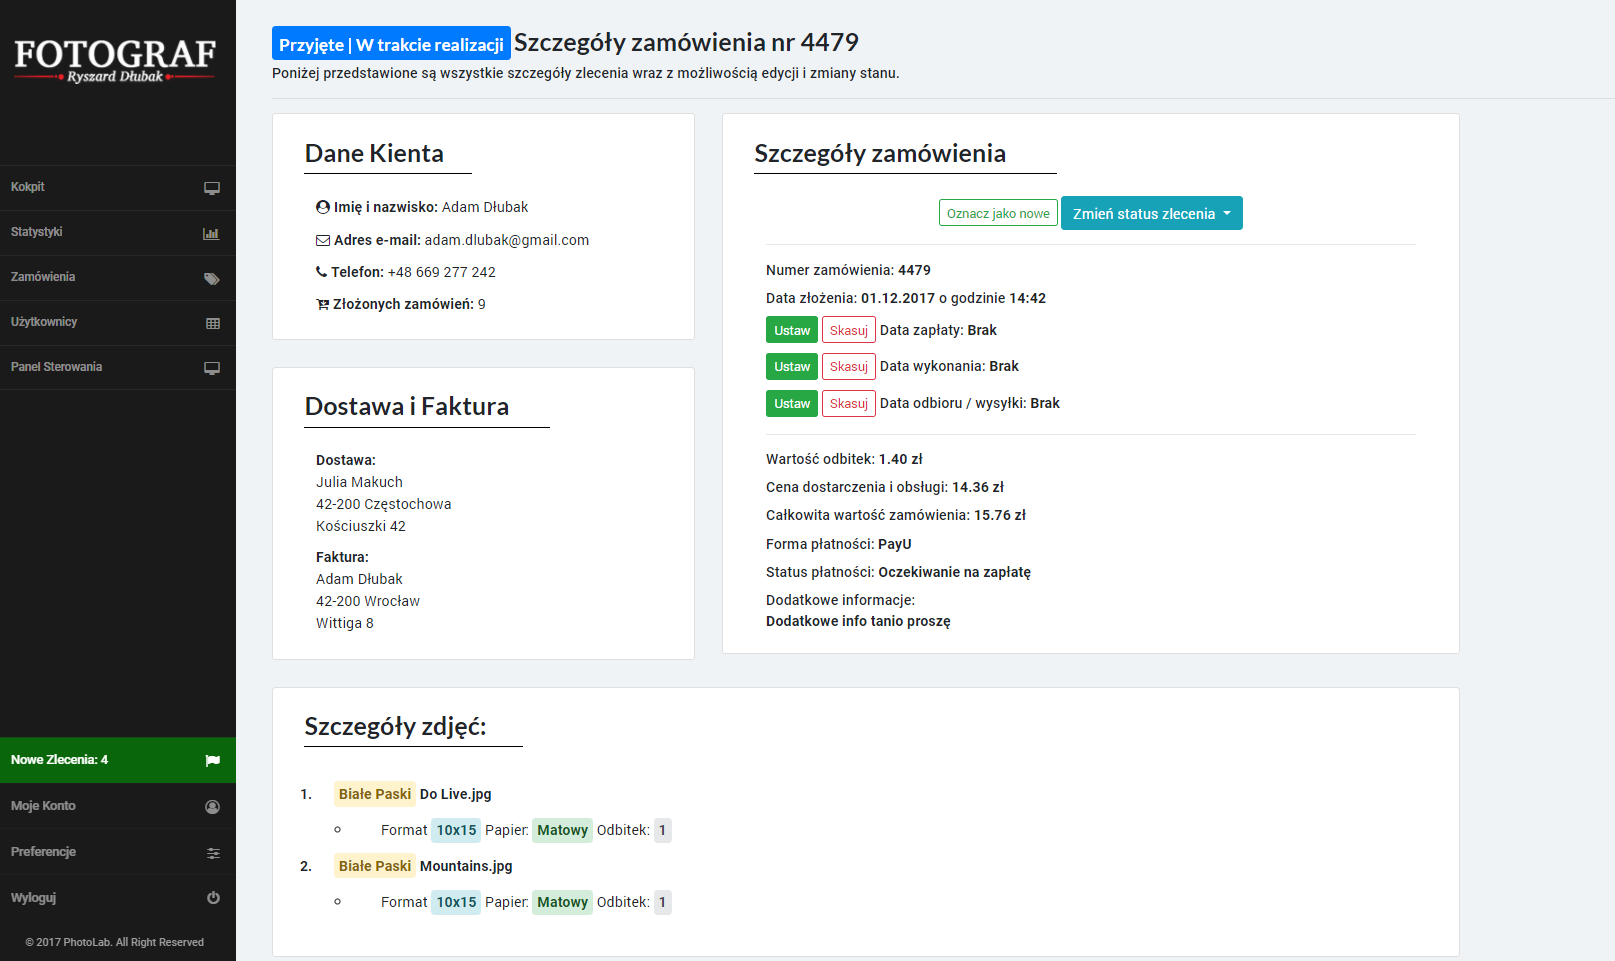
\includegraphics[width=0.9\linewidth]{graphics/chapter-4/screen-6.png}
	\caption{Widok szczegółów zamówienia w panelu administratora}
	\label{fig:screen-6}
\end{figure}

\noindent Ta podstrona ukazuje wszystkie dostępne informacje o zleceniu: podstawowe dane klienta, który je zlecił, a także informacje o adresie wysyłki i wystawieniu faktury. Z prawej strony, w sekcji \textit{szczegóły zamówienia}, administrator ma możliwość dokonania zmiany statusu zlecenia oraz uzupełnienia go o podanie daty jego przejścia do kolejnego etapu realizacji. Trzecią sekcją tego widoku jest część przeznaczona na szczegółowe rozpisanie wymagań dotyczących poszczególnych odbitek. To właśnie według tych treści, pracownik laboratorium realizuje zlecenie wydruku.

\noindent Ostatnim zademonstrowanym widokiem jest podstrona \textbf{panel sterowania}. Dzięki niej możliwa jest konfiguracja ogólnych ustawień serwisu takich jak: dostępne formaty wraz ze szczegółowym ich opisem, rodzaje papieru, czy domyślne ustawienia parametrów podczas dokonywania nowego zlecenia przez użytkowników. Interfejs zapewnia możliwość dodawania, usuwania (lub archiwizacji), a także pełnej edycji wszystkich przedstawionych poniżej ustawień.

\begin{figure}[ht]
	\centering
	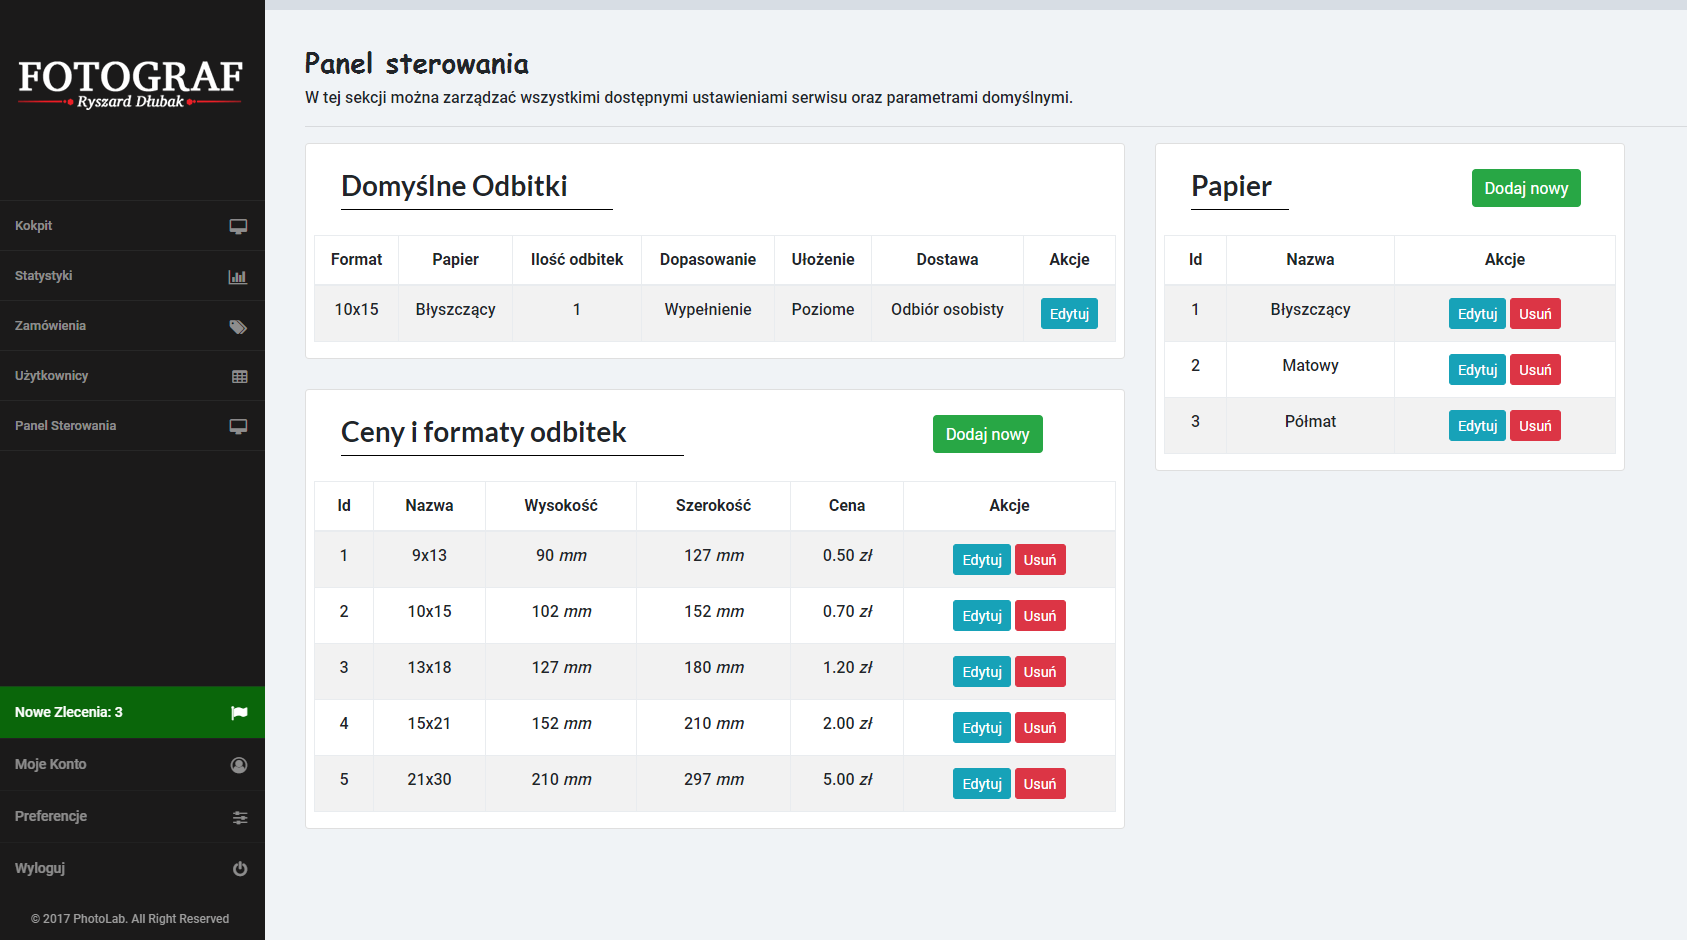
\includegraphics[width=0.9\linewidth]{graphics/chapter-4/screen-7.png}
	\caption{Widok modułu panelu sterowania ustawieniami serwisu}
	\label{fig:screen-7}
\end{figure}

\noindent Moduł administratora to również sekcja zarządzania własnym kontem, a także kontami użytkowników oraz panel statystyk. Nie są to jednak jego najważniejsza opcje, dlatego też zostaną ona pominięte, szczególnie, iż obsługa tej części jest bardzo prosta analogiczna do obsługi zleceń, jak i całego systemu.
\chapter{Testowanie}
{\em \quad Analiza zgodności aplikacji PhotoLab z przyjętymi wymaganiami jest głównym tematem tego rozdziału. Tematyka testów znajduje się tutaj jedynie w celu zasygnalizowania, iż takowe testy się odbyły i stanowią bardzo ważna część procesu wdrożenia każdego nowego oprogramowania. Zostaną tutaj przytoczone jedynie podstawowe informacje o przeprowadzonych testach i~~ich parametrach, a także najciekawsze spostrzeżenia i wnioski z nich płynące. Zabraknie natomiast wnikliwego przedstawienia całego procesu przeprowadzenia testów, ich szczegółowych parametrów i wnikliwej analizy. Nie jest to przedmiotem tego rozdziału jak i całej dokumentacji.}



\section{Testy funkcjonalne}
\quad Są to testy czarnej skrzynki (\textit{ang. black box testing}). Istnieje bardzo wiele rodzajów tego typu testów, w tym konkretnym wypadku polegały one na przetestowaniu bardzo ważnego elementu jakim jest \textit{API} serwera. Przed rozpoczęciem testów konieczne było przygotowanie odpowiednich danych. Były nimi parametry wejściowe zapytań kierowanych do serwera, takie jak: adres zapytania, nagłówki czy różne parametry, a także oczekiwane wzorcowe dane wyjściowe, do których następnie zostały porównane wszystkie otrzymane wyniki. Zawierały one zarówno poprawne, jak i błędne parametry. Miało to na celu sprawdzenie nie tylko poprawności zwracanych rezultatów, ale także weryfikacji sposobu obsługi błędów w przypadku wystąpienia błędnych zapytań. \\
\\
Wszystkie testy zostały oparte o bardzo prosty, jednakże niezwykle użyteczny program \textit{\textbf{Postman}}, służący właśnie do tego typu zadań. Przykładowa prezentacja testu jednego z zapytań znajduje się na  rysunku \ref{fig:functional-tests}. Dotyczy ona sprawdzania metody kontrolera odpowiedzialnej za rejestrację użytkownika. W tym konkretnym przypadku użytkownik wprowadził poprawne dane, a konto o podanym adresie jeszcze nie istniało w systemie. Otrzymany rezultat był zgodny z oczekiwanym.\\
\\
Testy wykazały kilka niewielkich niezgodności w zwracanych przez system odpowiedziach. Szybka weryfikacja pozwoliła naprawić dostrzeżone błędy i tym sposobem uniknąć ich na serwerze produkcyjnym. Ostatecznie wszystkie przeprowadzone testy zakończyły się sukcesem.

 \begin{figure}[ht]
	\centering
	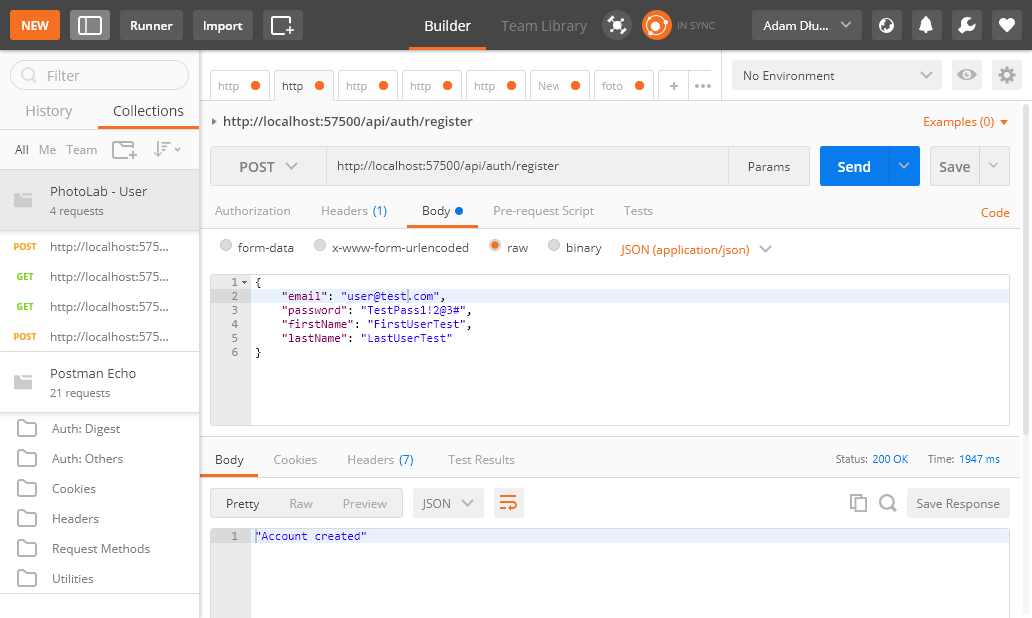
\includegraphics[width=1\linewidth]{graphics/chapter-5/functional-tests.png}
	\caption{Test funkcjonalny API z użyciem narzędzia PostMan}
	\label{fig:functional-tests}
\end{figure}


\newpage
\section{Testy użyteczności}
\quad W ramach testu przydatności i dostępności serwisu dla użytkowników zostały przeprowadzone testy użyteczności (\textit{ang. usability testing / user experience testing}). Podobnie do testów funkcjonalnych, również tego rodzaju testów istnieje wiele odmian i wariantów. Bardzo przykładem jest test typu \textit{eyetracking}, czyli badanie ruchu gałek ocznych, a zatem wędrówki wzroku użytkowników po serwisie www. Wynikiem takiego badania są tzw. \textit{head-mapy}, które pomagają określić np. na co na stronie największą uwagę zwracają klienci. Kolejnym interesującym testem jest nagrywanie zachowań osób odwiedzających witrynę. Specjalne narzędzie (np. aplikacja \textit{SmartLook}) wstrzyknięte w kod strony pozwala zapisywać każdy ruch użytkownika (ruchy myszki, wpisywane teksty, czy momenty zawahań i podejmowania decyzji). Powyższe sposoby nie zostały jednak wykorzystane do przeprowadzenia testów serwisu. Powodem ich dyskwalifikacji jest fakt, iż są to narzędzia wykorzystywane do badania stron, które zostały już opublikowane i korzysta z nich szerokie grono odbiorców. Wówczas analiza ich zachowań pozwala na modyfikację i podnoszenie jakości strony. \\
\\
W ramach badania użyteczności aplikacji \textit{PhotoLab} zdecydowano się na przeprowadzenie testów wykrywających obszary utrudniające realizację głównych założeń aplikacji oraz wpływających na negatywne odczucia użytkowników w trakcie korzystania ze strony.\\
Grupa testowa składała się z 6 osób - jest to liczba dość mała, jednak warunki projektowe nie pozwoliły przeprowadzić badań na większej grupie. Badani to 3 osoby w wieku 20-25 lat, 2~w przedziale 35-40 lat oraz jedna w wieku wyższym niż 55 lat - można również przyjąć, iż poziom znajomości obsługi komputerów był liniowo zależny do wieku użytkowników - osoba najstarsza posiadała najmniejszą wiedzę, najmłodsze - największą. Badani mieli do wykonania jeden zaplanowany scenariusz: wejście na stronę, zarejestrowanie nowego konta, zalogowanie użytkownika, zlecenie nowego zamówienia i ostatecznie z poziomu panelu użytkownika sprawdzenie statusu swojego zlecenia. Badanymi parametrami były między innymi: potrzebny czas na wykonanie scenariusza, popełnione błędy (podanie błędnych wartości, zagubienie na stronie, brak wiedzy o koniecznych do podjęcia kolejnych krokach, itp.), czy ogólne odczucia osób testujących.\\
\\
W ramach przedstawienia rezultatów przeprowadzonego testu można stwierdzić, iż ogólne odczucia badanych osób były bardzo pozytywne. Wszyscy użytkownicy samodzielnie ukończyli cały scenariusz w zbliżonym czasie (jedynie tester w wieku 55 lat rażąco odstawał od całego grona użytkowników - potrzebował dwukrotnie dłuższy czas niż najmłodsi, co jednak jest logiczne i nie jest specyfiką tylko aplikacji \textit{PhotoLab}). Przedstawiono także możliwości poprawy użyteczności głównie poprzez reorganizację kilku elementów strony. Zostały one uwzględnione i prawie wszystkie wdrożone (za wyjątkiem dwóch, które z technicznego punktu widzenia znacząco skomplikowałyby proces obsługi klienta).\\
\\
Test użyteczności zakończył się pozytywnym rezultatem. Wykazał kilka drobnych, wcześniej niedostrzeżonych elementów, które były stworzone nieoptymalnie dla potencjalnego klienta serwisu. Końcowe odczucia użytkowników były bardzo dobre, a sam system określony został jako przyjazny i przystępny dla każdego.

\section{Testy wydajnościowe}
\quad W ramach testów sprawdzających wydajność systemu zostały przeprowadzone 2 typy pomiarów: testy obciążenia (uwzględniające również test maksymalnego obciążenia) oraz testy wydajnościowe, które były zdecydowanie ważniejszym typem pomiarów. Testy uwzględniały naprzemienne wykonywanie dwóch scenariuszy biznesowych:
\begin{enumerate}
    \item Logowanie użytkownika i zlecania zamówienia.
    \item Logowanie administratora, przeglądanie wygenerowanych zleceń i ich edycja.
\end{enumerate}
Środowisko, które zostało wykorzystane do przeprowadzenia badań to w głównej mierze oprogramowanie \textit{Visual Studio} w wersji \textit{Enterprise 2017}, gdyż tylko taka wersja umożliwia wygenerowanie projektu typu \textit{Web Performance and Load Test Project}. Dodatkowo, aby nagrać scenariusz testowy zostało użyte oprogramowanie marki \textit{Telerik} - \textit{Fiddler}. Teoretycznie \textit{Visual Studio} zapewnia możliwość nagrywania scenariuszy poprzez wtyczkę do przeglądarki \textit{Internet Explorer 11}, jednakże nie spełniała ona swojej funkcji i została zastąpiona dodatkowym oprogramowaniem.\\
\\
Najważniejszym wynikiem przeprowadzonych testów było wykrycie błędu aplikacji będącej pod dużym obciążeniem. Serwis, z którego korzystało około 300 użytkowników jednocześnie rozpoczął generowanie błędów z serii \textit{500} - \textit{Internal Server Error}. Oznaczało to, iż stworzona aplikacja posiada wewnętrzny błąd, który ujawnia się dopiero przy dużym obciążeniu serwera (rys. \ref{fig:load-test-result-before-repair}).\\
\\
Analiza logów serwera wykazała, iż problem występuje w związku z połączeniem z bazą danych wychodzącym z kontrolera odpowiedzialnego za logowanie użytkownika. Polegał on na otwarciu zbyt wielu (ustawienia serwera ograniczały ilość do 100) aktywnych połączeń z bazą danych oczekujących asynchronicznie na jej odpowiedź. Pierwszym możliwym, chociaż niezalecanym sposobem uniknięcia tego błędu jest zwiększenie domyślnego parametru otwartych połączeń z bazą danych (\textit{ang. max pool size}). Nie jest to jednak rozwiązanie dobre, gdyż jak wynika z dokumentacji tej technologii, domyślna liczba w zupełności wystarcza nawet dużym i~obciążonym systemom. Należało wiec poszukać błędu w samym kodzie metody \textit{login()}. Jak się ostatecznie okazało, faktycznie występowało tam redundantne odpytywanie bazy danych o~dane użytkownika. Wynikało to z faktu, iż metoda ta zawierała zarówno kod biblioteki \textit{ASP.NET Identity}, a także generator kluczy \textit{JWT} i wystąpił tutaj typowy błąd programistyczny niepoprawnie stworzonej obsługi zapytania. Po dokonaniu odpowiednich modyfikacji i~ponownym przetestowaniu aplikacji okazało się, iż problem został wyeliminowany, a~poza uniknięciem generowanie błędów stanowczo zmalało również obciążenie procesora (rys. \ref{fig:load-test-result-after-repair}).
 \begin{figure}[ht]
	\centering
	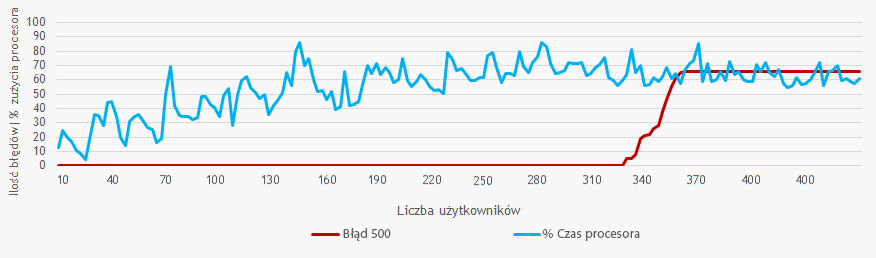
\includegraphics[width=1\linewidth]{graphics/chapter-5/load-test-result-before-repair.png}
	\caption{Test obciążenia serwera po wykryciu błędów typu 500}
	\label{fig:load-test-result-before-repair}
\end{figure}
 \begin{figure}[ht]
	\centering
	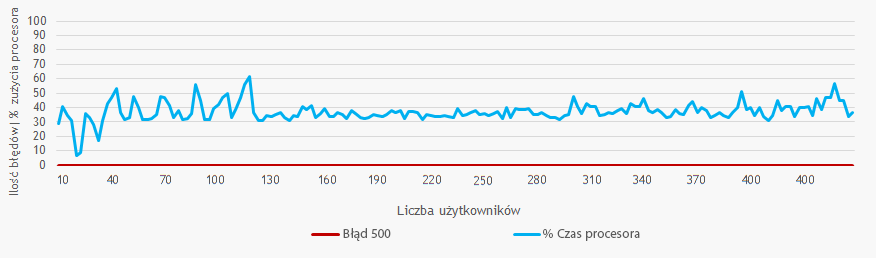
\includegraphics[width=1\linewidth]{graphics/chapter-5/load-test-result-after-repair.png}
	\caption{Test obciążenia serwera po eliminacji błędów typu 500}
	\label{fig:load-test-result-after-repair}
\end{figure}


\noindent Udało się również przeprowadzić testy wydajności niektórych, najważniejszych, zapytań serwera takich jak: \textit{getOrders()}, \textit{getUsers()}, \textit{submitOrder()}. Wykazały one, iż zapytania obsługiwane są w zadowalającym czasie. Jedynym \textit{requestem}, który znacznie odbiegał czasem odpowiedzi od pozostałych było zapytanie z prośbą o zwrócenie wszystkich znajdujących się w systemie zamówień. Udało się je jednak zoptymalizować poprzez skonkretyzowanie zwracanych informacji i znaczne zmniejszenie ich liczby, która była zbędna i nie wykorzystywana przez aplikację kliencką.
\newpage

\vspace*{0.01\baselineskip}

\section{Zgodność z wymaganiami}
\quad W momencie, gdy aplikacja została już w pełni zbudowana oraz przetestowana można określić jej poziom zgodność z założonymi w pierwszym etapie realizacji wymaganiami.\\
\\
Rozpoczynając podsumowanie od założeń technicznych należy stwierdzić, iż wykorzystanie wszystkich planowanych technologii, a także architektury trójwarstwowej zostało spełnione. W trakcie realizacji projektu nie napotkano na problemy, które mogłyby spowodować konieczność zmiany podejścia do architektury lub technologii. Jedynym odstępstwem jest zaimplementowanie serwera aplikacji w technologii \textit{.Net Core} w wersji \textit{2.0}, która jest wersją nowszą od planowej \textit{1.1}, a która w momencie projektowania była najnowszą wersją (dlatego też wersja \textit{2.0} nie została wówczas uwzględniona).\\
\\
Mówiąc o kompletności spełnienia założeń funkcjonalnych również można powiedzieć o~pełnym sukcesie. Udało się zaimplementować wszystkie funkcjonalności podstawowe, a~także planowane jako opcjonalne - funkcjonalności dodatkowe. Mimo ograniczonych ram czasowych na realizację projektu, szybki postęp prac pozwolił skupić się na implementacji wszystkich zakładanych funkcji systemu.\\
\\
Ostatnim, a zarazem najważniejszym wymogiem projektu było spełnienie jego czterech podstawowych celów. Były to: prostota użytkowania, przystępny koszt wdrożenia i utrzymania, bezpieczeństwo danych i transakcji oraz pokrycie wszystkich funkcjonalności oferowanych przez laboratorium w aplikacji internetowej. \\
\\
Analizując kolejno każdy z wymogów można stwierdzić iż:
\begin{enumerate}
    \item Przeprowadzone testy użyteczności wykazały łatwą dostępność, prostotę interfejsu i pozytywne wrażenia estetyczne budowanego serwisu podtrzymując przy tym tezę, iż użytkowanie systemu jest bezproblemowe.
    \item Jednoosobowy zespół projektowy, krótki okres wdrożenia (około 2 miesiące) i bardzo tani lub wręcz darmowy hosting przemawiają za tym, iż koszta poniesione na realizację autentycznego projektu nie mogłyby być wygórowane.
    \item Zaimplementowanie biblioteki \textit{ASP.NET Identity} oraz standardu \textit{JWT Token}, a także przeprowadzenie testów zarówno funkcjonalnych jak i wydajnościowych powoduje, iż aplikacja posiada wysoki (jak na możliwości projektowe i nakład środków) poziom zabezpieczeń.
    \item Ponieważ cały możliwy zakres oferty laboratorium został ustalony i spisany w formie funkcjonalności podstawowych i rozszerzonych, które z kolei zostały kompletnie zaimplementowane należy uznać, iż projekt spełnia również założenia ostatniego celu - pokrycia oferty zakładu w formie stacjonarnej, funkcjonalnościami serwisu online.
\end{enumerate}


\chapter{Podsumowanie}
    {\em \quad Proces planowania, budowania oraz testowania aplikacji PhotoLab dobiegł końca. W rozdziale tym zostanie podsumowana wykonana praca oraz nastąpi porównanie produkt końcowego z jego wstępnymi założeniami. Dodatkowo omówione będą możliwości dalszego rozwoju i rozszerzania funkcjonalności aplikacji. Na sam koniec rozpisane zostaną wnioski, które nasunęły się w trakcie trwania projektu jak i podczas użytkowania i testowania produktu finalnego.}
    
\section{Efekt końcowy}
\quad Ostatecznie pomimo wielu problemów i przeciwności udało się zakończyć proces budowania aplikacji. Efektem prac jest aplikacja internetowa dostępna dla każdego zainteresowanego użytkownika z poziomu przeglądarki internetowej - zarówno z komputerów klasy PC jak i~urządzeń mobilnych. \\
\\
Zanim zostanie omówione to, co udało się zrobić w ramach projektu, warto przyjrzeć się napotkanym błędom i trudnościom.\\
Pierwszym problemem, który pojawił się już w początkowej fazie procesu implementacji było zbudowanie odpowiedniego środowiska, w którym mógłby być budowany projekt. Wariantów było kilka, trzy z nich zostały przetestowane i spośród nich wybrano ostatecznego zwycięzcę. Pierwszym wyborem było gotowe środowisko wraz z przykładową aplikacją oferującą wprost ,,z pudełka'' bardzo wiele możliwości. Niestety jak się okazało, zbyt wiele, a w dodatku takich, które nie zostałyby wdrożone w aplikacji \textit{PhotoLab}. Projekt ten choć z założenia służył jako ,,aplikacja startowa'' dla nowych projektów, okazał się zbyt przeładowany niepotrzebnymi funkcjami oraz napisany w niespójny i nieuporządkowany sposób, a w dodatku bez dokumentacji projektowej, przez co był bardzo trudny do zrozumienia i dalszej pracy nad nim. \\
Kolejny wybór padł na podstawowy szablon generowany z poziomu tworzenia nowego projektu aplikacji \textit{Visual Studio} - \textit{AngularSPA}. Projekt ten automatycznie generował podwaliny pod aplikację opartą o \textit{Angular'a} po stronie klienta oraz \textit{ASP.NET Core} po stronie serwera. Problemem jednak okazał się mało przejrzysty schemat łączenia obu aplikacji, które mocno zazębiały się swoją strukturą i odpowiedzialności. Dodatkowo \textit{Angular} oparty był na generowaniu po stronie serwera (\textit{ang. Server Side Rendering (SSR)}), nie natomiast po stronie przeglądarki internetowej (utrudniając przez to dostęp do takich funkcjonalności jak np. pamięć lokalna przeglądarki), jak było to zakładane i wymagane dla wdrażanej aplikacji. Dodatkowym problem okazało się narzędzie \textit{WebPack} służące do zarządzania zależnościami między modułami i budowania aplikacji. Nie było ono proste, ani intuicyjne dla programisty, przez co okazało się kolejnym powodem do wycofania się z implementacji tej struktury projektowej. \\
Trzeci wybór, który okazał się wyborem ostatecznym, padł na osobne wygenerowanie aplikacji serwerowej \textit{ASP.NET Core Web API} z poziomu interfejsu środowiska programistycznego \textit{Visual Studio 2017} oraz aplikacji klienckiej. Ta druga powstała w oparciu o bardzo proste narzędzie konsolowe \textit{Anglular CLI}, które nie tylko pomogło wygenerować projekt warstwy prezentacji ale także odpowiednio nim zarządzać. Struktura projektowa utworzona za pomocą tego narzędzia choć do zarządzania zależnościami również korzystała z narzędzia \textit{Webpack}, to było ono obudowane dodatkowym uproszczonym interfejsem \textit{CLI}, który w zupełności wystarczył na potrzeby projektu, natomiast znacznie uprościł proces przygotowywania środowiska.\\
\\
Już na etapie końca implementacji zasadniczej części warstwy serwerowej została podjęta decyzja o aktualizacji \textit{ASP.NET Core} do najnowszej wersji, która w tamtym czasie się pojawiła - wersji \textit{2.0} (z \textit{v1.1}). Miała to być drobna zmiana, nie mająca większego wpływu na obecnie stworzony kod. Rzeczywistość okazała się jednak inna. W implementacji wielu metod, struktur i bibliotek zaszły zmiany (często bardzo drobne), które jednak powodowały, że już wcześniej napisany kod przestał działać. Dość sporą ilość czasu zajęło przywrócenie wcześniej już zaimplementowanych funkcjonalności. Dodatkowo późniejsze budowanie kolejnych elementów serwera okazało się być trudniejsze, niż się spodziewano. W związku z~pracą w~dopiero co wdrożonej wersji technologii, wiele problemów dla których rozwiązanie można bardzo szybko znaleźć w Internecie, okazało się problemami, które należy rozwiązać samemu. Było to spowodowane brakiem stosownej dokumentacji, poradników i ogólnego \textit{community}.\\
\\
Ostatni z poważnych problemów został napotkany na etapie wdrożenia projektu na serwer produkcyjny. Napotkano wówczas na wiele trudności, niezgodności i braków kompatybilności. Ponieważ środki dostępne na wdrożenie były mocno ograniczone, zakres możliwości dotyczący wyboru konkretnych ofert hostingowych również był bardzo wąski. Dodatkowo połączenie aplikacji opartej o dwie różne technologie - \textit{.Net} i \textit{Javascript} nie ułatwiał tego zadania. Pierwsze próby zakładały upublicznienie aplikacji \textit{PhotoLab} jako jednej, scalonej aplikacji. Niestety w~tym wariancie wystąpiło wiele problemów związanych z przekierowywaniem połączeń, wysyłaniem zapytań \textit{HTTP} oraz ogólnym \textit{routingem} aplikacji. Wówczas została podjęta o~osobnym wystawieniu aplikacji klienckiej oraz serwerowej z bazą danych. Po rozwiązaniu pomniejszych problemów rozwiązanie to okazało się poprawne, a wdrożenie zakończyło się pełnym sukcesem.\\
\\
Określając ostateczny efekt projektu należy powiedzieć, iż została zbudowana średnich rozmiarów, \textit{responsywna} aplikacja webowa, której struktura oparta jest o model trójwarstwowy. Interfejs klienta jest przyjazny i łatwy w użytkowaniu, co zostało przetestowane i wykazane w~trakcie przeprowadzania testów użyteczności. Część serwerowa jest spójna i zabezpieczona. Testy wydajnościowe wykazały lukę w jej budowie, która została poprawiona, a ponownie przeprowadzone badania potwierdziły jej odporność na błędy i optymalność działania przy maksymalnym zakładanym obciążeniu.

\section{Możliwości dalszego rozwoju aplikacji}
\quad Aplikacja \textit{PhotoLab} nie jest produktem ostatecznym. Można oznaczyć ją jako wersję \textit{1.0} z~możliwością dalszego rozwoju. Zarówno w trakcie implementacji, jak i w czasie testowania produktu końcowego zauważono bardzo wiele możliwości rozbudowy, modyfikacji lub poprawienia niektórych rozwiązań, a także dodania nowych funkcjonalności. \\
\\
Listę pomysłów i możliwości na dalszy rozwój aplikacji warto rozpocząć od zidentyfikowanych części aplikacji, które wymagają udoskonalenia lub rozbudowy. Z pewnością należą do nich:
\begin{itemize}
    \item Operacje na przesyłanych zdjęciach - obecnie jedyną możliwością edycji zdjęcia przed ich przesłaniem do laboratorium jest ustalenie sposobu dopasowania (białe paski lub wypełnienie) oraz orientacji (pionowej lub poziomej). Moduł ten można by rozszerzyć o takie funkcjonalności jak: przycinanie zdjęć w wizualnym edytorze na żywo, sterowanie kolorystyką zdjęcia (nasycenie, kontrast) oraz gotowe \textit{presety} takie jak: czerń i biel, sepia czy negatyw.
    \item Źródło pochodzenia zdjęć - z pewnością ciekawym dodatkiem byłaby możliwość przesyłania zdjęć do wydruku nie tylko z urządzenia, na którym otwarta jest aplikacja ale również z popularnych portali społecznościowych, czy dysków internetowych (\textit{DropBox}, \textit{Google Drive}, \textit{Mega.nz} etc.).
\end{itemize}

\quad Aplikacja została oparta o architekturę, która umożliwia jej łatwy rozwój, w ramach którego możliwe jest dobudowywanie nowych modułów i funkcjonalności. Kilka propozycji, które nasunęły się podczas testów aplikacji to:
\begin{itemize}
    \item Rejestracja użytkowników - bardzo użytecznym dodatkiem w kolejnej wersji aplikacji byłaby z pewnością możliwość rejestracji jak i logowania użytkowników poprzez popularne portale takie jak \textit{Facebook} czy \textit{Google}. Z pewnością ułatwiło i przyspieszyłoby to proces rejestracji nowych użytkowników.
    \item Dokonywanie płatności - rozszerzenie możliwości np. poprzez system \textit{PayU} lub \textit{PayPal}. Ulepszyłoby to proces opłacania nowych zamówień, a przez to również skróciło czas ich realizacji.
    \item Moduł mailingowy - część aplikacji odpowiedzialna za wszelkiego rodzaju maile rozsyłane w ramach usług serwisu. W celu poinformowania klienta o etapie realizacji zlecenia mógłby być generowany automatyczny mail informacyjny lub administrator systemu z poziomu swojego kokpitu mógłby wysyłać spersonalizowane maile oparte o przygotowane szablony.
\end{itemize}
Jak widać, poprzez zaprezentowane przykłady i pomysły, możliwości kontynuacji prac nad rozwojem kolejnych wersji aplikacji \textit{PhotoLab} jest bardzo wiele. Jedne z nich są bardziej użyteczne, inne mniej, jednak każde wnoszą nowe wartości i możliwości dla funkcjonowania strony. 

\section{Wnioski}
\quad Projekt aplikacja \textit{PhotoLab}, oficjalnie nazwany jako: ,,System do obsługi laboratorium fotograficznego z możliwością sprzedaży foto usług online'', zakończył się sukcesem. Wszystkie zaplanowane funkcjonalności, zarówno podstawowe jak i rozszerzone zostały zaimplementowane i wdrożone w środowisku produkcyjnym. Aplikacja została zbudowana w oparciu o~architekturę, którą starannie zaplanowano już w czasie przygotowań. Strona \textit{PhotoLab} ma dokładnie taką formę i prezencję, jak zostało to uprzednio ustalone. Wszystkie przeprowadzone testy zarówno wydajnościowe, jak i funkcjonalne zakończyły się sukcesem, a testy użyteczności zostały pomyślnie zaakceptowane przez biorących w nich udział użytkowników.\\
\\
Projekt, chociaż zakończony sukcesem, okazał się bardzo trudny i wymagający. Nie obyło się bez wielu problemów i trudności, które zostały dokładnie opisane w \textit{rozdziale 6.1}. Do najważniejszych z nich z pewnością należy zaliczyć aktualizację środowiska serwerowego ASP.NET Core z wersji \textit{1.1} do \textit{2.0}, a także wdrożenie projektu na serwer produkcyjny.\\
\newpage
\noindent Patrząc na cały projekt z perspektywy już gotowego i wdrożonego rozwiązania można stwierdzić, iż bardzo dobrym wyborem było zastosowanie technologii \textit{Angular}. Jest ona niezmiernie szybka i wprowadza  możliwości podejmowania licznych interakcji użytkownika ze stroną poprzez zastosowanie funkcjonalności \textit{two way data binding}. Jednocześnie jest relatywnie prosta we wdrożeniu i implementacji - głównie poprzez zastosowanie narzędzia \textit{Angular CLI}.\\
\\
Analizując stronę serwera aplikacji można z jednej strony zastanawiać się nad słusznością aktualizacji wersji w trakcie implementacji projektu, z drugiej - być bardzo zadowolonym z wyboru jednej rodziny rozwiązań do implementacji zarówno serwera, jak i warstwy bazy danych. Z pewnością umożliwiło to uniknięcia problemów z brakiem odpowiedniego współdziałania i wymiany informacji. Zastosowanie narzędzia klasy \textit{ORM}, \textit{Entity Framework}, znacznie ułatwiło i przyspieszyło czas implementacji, dodatkowo udostępniając bardzo łatwy, prosty i intuicyjny sposób operowania na modelach zarówno dla strony serwera. jak i bazy danych, unikając w ten sposób konieczności posługiwania się kolejnym językiem programowania jakim jest \textit{SQL}.\\
\\
Podsumowując projekt można stwierdzić, iż wszystkie założone funkcjonalności, zarówno podstawowe, jak i rozszerzone zostały zaimplementowane i wdrożone. \textit{PhotoLab} jest w pełni funkcjonalnym systemem zlecania zamówień wydruku zdjęć online dającym użytkownikowi możliwość w łatwy i przyjazny dla niego sposób zapoznać się z firmą oraz jej obszarem działalności, a także skorzystać z oferowanych przez nią usług bez wychodzenia z domu.


\appendix


\nocite{*}
\bibliographystyle{unsrt}
\bibliography{bibliography}


\chapterstyle{noNumbered}
\phantomsection % sets an anchor
\addcontentsline{toc}{chapter}{Indeks rzeczowy}
\printindex


\newpage
\mbox{}\pdfbookmark[0]{Spis rysunków}{spisRysunkow.1}
%\addcontentsline{toc}{chapter}{Spis rysunków}
\listoffigures*
\begin{flushleft}

\end{flushleft}
%{%
%\let\oldnumberline\numberline%
%\renewcommand{\numberline}{\figurename~\oldnumberline}%
%\listoffigures%
%}


\newpage

% %\addcontentsline{toc}{chapter}{Spis tabel}
% \listoftables*

\newpage
\renewcommand\listoflistingscaption{Spis listingów}
\listoflistings

% \chapter*{Słownik pojęć i skrótów}\mbox{}\pdfbookmark[0]{Słownik pojęć i skrótów}{skroty.1}
\label{sec:skroty}
\noindent
\begin{description}
  \item [SPA] (ang.\ \emph{Single Page Application})
  \item [MVC] (ang.\ \emph{Model-View-Controller})
  \item [DOM] (ang.\ \emph{Document Object Model})
  \item [OOP] (ang.\ \emph{Object Oriented Programming})
  \item [DRY] (ang.\ \emph{Don't Repeat Yourself})
  \item [CLR] (ang.\ \emph{Common Language Runtime})
  \item [ORM] (ang.\ \emph{Object-Relational Mapping})
  
  
%  \item [Licencja MIT]
%  \item [PhotoLab]
%  \item [Framework] 
%  \item [Frontend]
% \item [Backend]
%  \item [Community]
\end{description}
 %skróty można sobie pominąć


\end{document}
